\documentclass[12pt,a4paper]{report}

% ── Pacchetti di base ────────────────────────────────────────────────────
\usepackage[utf8]{inputenc}
\usepackage[T1]{fontenc}
\usepackage[italian]{babel}
\usepackage[a4paper,margin=3cm]{geometry}
\usepackage{lmodern}
\usepackage{amsmath,amssymb}
\usepackage{mathrsfs}
\usepackage{graphicx}
\usepackage{subcaption}
\usepackage{booktabs}
\usepackage{rotating}
\usepackage{multirow}
\usepackage[expansion=false,nopatch=footnote]{microtype}
\usepackage{xcolor}
\usepackage{hyperref}
\usepackage{cleveref}
\usepackage[authoryear,round]{natbib}
\setlength{\marginparwidth}{2cm}
\usepackage[colorinlistoftodos]{todonotes}

% ── Link interni colorati ma senza le cornici colorate di default di
% hyperref (poco eleganti in stampa/PDF): colore unico, sobrio, per
% riferimenti, citazioni e URL ────────────────────────────────────────
\definecolor{linknavy}{RGB}{20,50,110}
\hypersetup{
  colorlinks=true,
  linkcolor=linknavy,
  citecolor=linknavy,
  urlcolor=linknavy,
  linktoc=all
}
\usepackage{setspace}
\onehalfspacing % interlinea 1.5
\usepackage{listings}

% ── Stile per i listati di codice (sobrio: monocromatico, leggibile anche
% in stampa b/n, coerente con una tesi ingegneristica) ──────────────────
\definecolor{listinggray}{gray}{0.95}
\definecolor{listingcomment}{gray}{0.45}
\lstdefinestyle{thesiscode}{
  backgroundcolor=\color{listinggray},
  basicstyle=\ttfamily\small,
  commentstyle=\color{listingcomment}\itshape,
  keywordstyle=\bfseries,
  numbers=none,
  frame=single,
  rulecolor=\color{gray!60},
  framerule=0.4pt,
  breaklines=true,
  showstringspaces=false,
  columns=flexible,
  xleftmargin=1em,
  xrightmargin=1em,
  aboveskip=1em,
  belowskip=1em,
  language=bash
}
\lstset{style=thesiscode}

\graphicspath{{img/}{../results/plots/compare_3stat/}{../results/plots/differenza_percentuale/}{../results/plots/}}

% ── NOTA SU QUESTO FILE ──────────────────────────────────────────────────
% "mainquasiufficiale.tex" e' il file ufficiale della tesi (main.tex resta
% come backup della versione precedente). Compila per intero i capitoli 1
% (Introduzione), 2 (Background) -- riscritti -- e 5 (Conclusioni) -- nuovo
% -- insieme ai capitoli 3 e 4 (identici a quelli di main.tex), cosi' che
% numerazione, citazioni e riferimenti incrociati risultino corretti.
% Le pagine dei capitoli 3 e 4 vengono poi rimosse meccanicamente dal PDF
% finale (script scratchpad, pypdf): e' l'unico modo per avere "si puo'
% citare il capitolo 3 anche se il capitolo 3 non c'e' nel pdf" con
% riferimenti numerici garantiti corretti.

% ── Dati del frontespizio ──────────────────────────────────────────────
\newcommand{\nomeUniversita}{Università di Firenze}
\newcommand{\nomeDipartimento}{Scuola di Scienze Matematiche Fisiche e Naturali}
\newcommand{\nomeCorso}{Laurea Magistrale in Data Science, Calcolo Scientifico \& Intelligenza Artificiale}
\newcommand{\nomeRelatore}{Daniele Castellana}
\newcommand{\nomeCandidato}{Alessio Minati}
\newcommand{\annoAccademico}{2025/2026}

\title{Apprendimento per Rinforzo Multi-Agente basato su Reti Neurali a Grafo per il Controllo Semaforico}
\author{}
\date{}

\begin{document}

% ── Frontespizio ─────────────────────────────────────────────────────────
\begin{titlepage}
  \centering
  \vspace*{0.5cm}
  {\large \nomeUniversita \par}
  \vspace{0.15cm}
  {\large \nomeDipartimento \par}
  \vspace{0.15cm}
  {\large \nomeCorso \par}

  \vspace{2.2cm}
  \rule{\textwidth}{0.6pt}\par
  \vspace{0.5cm}
  {\Huge \bfseries Apprendimento per Rinforzo Multi-Agente basato su Reti Neurali a Grafo per il Controllo Semaforico \par}
  \vspace{0.5cm}
  \rule{\textwidth}{0.6pt}\par

  \vspace{1cm}
  {\Large \bfseries [DOCUMENTO DI LAVORO -- QUASI-UFFICIALE] \par}
  {\normalsize Capitoli 1, 2 e 5 in versione rivista; capitoli 3 e 4 identici a main.pdf \par}

  \vspace{1.5cm}
  \begin{minipage}[t]{0.47\textwidth}
    \raggedright
    \large\textbf{Relatore}\par
    \normalsize\nomeRelatore\par
  \end{minipage}
  \hfill
  \begin{minipage}[t]{0.47\textwidth}
    \raggedleft
    \large\textbf{Candidato}\par
    \normalsize\nomeCandidato\par
  \end{minipage}

  \vfill
  {\large Anno Accademico \annoAccademico \par}
  \vspace{0.5cm}
\end{titlepage}

\newpage
\thispagestyle{empty}
\null
\newpage

% ── Front matter: numerazione romana ─────────────────────────────────────
\pagenumbering{roman}

%!TEX root = ../main.tex
\chapter*{Sommario}
\addcontentsline{toc}{chapter}{Sommario}

Un incrocio semaforico deve garantire un flusso regolare dei veicoli che
vi transitano. Le soluzioni classiche affrontano il problema attraverso
un piano a tempi fissi, con fasi di durata prestabilita calcolata su
stime di traffico medie, oppure attraverso un controllo attuato dai sensori, che
concede il verde a una direzione solo quando un sensore rileva la
presenza di un veicolo in coda.

Quando gli incroci da controllare sono più di uno, emerge un problema
ulteriore: le decisioni prese a un incrocio devono essere coordinate con
quelle degli incroci vicini, perché il traffico smaltito da un'intersezione si riversa in
parte in quello in entrata ad un'altra intersezione. Sistemi come SCOOT e SCATS rispondono a
questa esigenza coordinando i piani semaforici di un'intera area urbana
sulla base del traffico osservato in tempo reale.

Entrambe le famiglie di soluzioni si basano però su euristiche definite
manualmente e restano per questo poco flessibili di fronte a condizioni di
traffico diverse da quelle previste in fase di progettazione. Il
reinforcement learning offre un'alternativa, apprendendo una
politica di controllo dall'esperienza simulata invece di codificarla
esplicitamente. MetaSTGAT (Wang et al., 2022) ne è un esempio, con un agente RL per
intersezione coordinato da una \emph{graph attention network} i cui pesi
sono generati dinamicamente da un modulo di meta-learning condizionato su
caratteristiche locali della rete stradale. Il lavoro originale si
concentra però sull'efficienza aggregata della rete, senza verificare se
il controllore generalizzi a topologie mai osservate in addestramento né
se il vantaggio ottenuto sia distribuito equamente tra le direzioni di
traffico servite.

Questo lavoro replica da zero l'architettura e la procedura di training
di MetaSTGAT, estendendola esplicitamente su questi due assi, equità e
generalizzazione, su un ambiente costruito su \textsc{CityFlow} con reti
a griglia di tre dimensioni ($4\times4$, $5\times5$, $6\times6$) e
traffico generato parametricamente.
Ogni differenza introdotta rispetto alla procedura originale è isolata da un
sistema di preset di ablazione e motivata singolarmente.

I risultati sperimentali confrontano le baseline classiche (Fixed-Time,
MaxPressure) con tre varianti del modello proposto che pesano
diversamente nella ricompensa la componente di equità, con uno studio di
ablazione completo e con un confronto tra tre meccanismi di comunicazione
spaziale alternativi. Il termine di ricompensa dedicato all'equità
risulta essere utile per il raggiungimento della stessa e
il meccanismo di comunicazione spaziale scelto si conferma efficace
per l'ottenimento di un buon coordinamento tra gli incroci della rete.


\tableofcontents
\listoffigures
\listoftables

%!TEX root = ../main.tex
\chapter*{Acronimi e Notazione}
\addcontentsline{toc}{chapter}{Acronimi e Notazione}

\section*{Acronimi}
\begin{table}[ht]
\centering
\small
\begin{tabular}{@{}ll@{}}
\toprule
Acronimo & Significato \\
\midrule
MDP & Markov Decision Process \\
RL & Reinforcement Learning \\
DQN & Deep Q-Network \\
PER & Prioritized Experience Replay \\
BPTT & Backpropagation Through Time \\
GNN & Graph Neural Network \\
GCN & Graph Convolutional Network \\
GAT & Graph Attention Network \\
TSC & Traffic Signal Control \\
SMK & Spatial Meta-Knowledge (learner) \\
TMK & Temporal Meta-Knowledge (learner) \\
CS & Cooperation Spatial (modulo Meta-GAT) \\
CST & Cooperation Spatial-Temporal (modulo Meta-GAT) \\
\bottomrule
\end{tabular}
\end{table}

\newpage
\section*{Notazione principale}
\begin{table}[ht]
\centering
\small
\begin{tabular}{@{}lp{10.5cm}@{}}
\toprule
Simbolo & Significato \\
\midrule
$\mathcal{S}, \mathcal{A}, P, R, \gamma$ & Stati, azioni, transizione, ricompensa, sconto \\
$\pi$, $V^\pi$, $Q^\pi$ & Politica, funzione valore-stato, funzione valore-azione \\
$\theta$, $\theta^-$ & Pesi della rete online e della target network \\
$\tau$ & Coefficiente di soft update \\
$\alpha$ (in RL) & Esponente di prioritizzazione del PER \\
$\alpha$ (in questo lavoro) & Peso della penalità anti-starvation nella ricompensa \\
$\varepsilon$ & Probabilità di esplorazione \\
$s_i^t, a_i^t, r_i^t$ & Stato, azione, ricompensa dell'intersezione $i$ al tempo $t$ \\
$n_i^t, w_i^t, p_i^t$ & Veicoli per corsia, attesa massima per corsia, fase corrente \\
$d_0$ & Dimensione dello stato in ingresso \\
$d_1$ & Dimensione nascosta del modello \\
$H$, $d_h$ & Numero di teste di attenzione e dimensione per testa \\
$e_i^t, e_j^t$ & Embedding temporale e spaziale del Dual State Encoder \\
$x_i^t, h_i^t, c_i^t$ & Output, stato nascosto e stato di cella del Meta-LSTM \\
$\mathrm{SMK}(i), \mathrm{TMK}(i)$ & Meta-embedding spaziale e temporale dell'intersezione $i$ \\
$z_{\mathrm{CS}}(i), z_{\mathrm{CST}}(i)$ & Output dei moduli Meta-GAT spaziale e spazio-temporale \\
$\overline{tt}$, $tt_{\max}$ & Travel time medio e massimo \\
$tc$ & Trip completion, percentuale di veicoli che completano il percorso \\
$\text{wait}_{\max}$ & Max wait, tempo massimo di un veicolo sulla stessa corsia senza superare l'incrocio \\
\bottomrule
\end{tabular}
\end{table}


% ── Corpo della tesi: numerazione araba da qui ────────────────────────────
\cleardoublepage
\pagenumbering{arabic}

%!TEX root = ../main.tex
\chapter{Introduzione}
\label{cap:introduzione}

\section{Motivazioni}
\label{sec:intro-motivazioni}

Un incrocio semaforizzato stabilisce periodicamente quali flussi veicolari
autorizzare e quali arrestare. Su una singola intersezione il problema è
garantire che i veicoli in attesa continuino a scorrere in modo regolare.
Le soluzioni classiche affrontano questo compito in due modi. Un piano a
tempi fissi ripete una sequenza di fasi di durata prestabilita, calcolata
una tantum su stime di traffico medie e mai più rivista in tempo reale. Un
controllo attuato dai sensori concede invece il verde a una direzione solo
quando un sensore rileva la presenza di un veicolo in coda, adattandosi
così, entro certi limiti, alle variazioni del traffico osservato.

Se si considera una rete composta da più incroci, il problema cambia
natura. La fase scelta a un'intersezione influenza, con un ritardo
proporzionale alla distanza, il volume di veicoli in arrivo alle
intersezioni adiacenti, per cui le decisioni prese nei singoli punti della
rete non possono più essere indipendenti tra loro. Sistemi come SCOOT e
SCATS rispondono a questa esigenza da diversi decenni, aggiustando
periodicamente i piani semaforici di un'intera area urbana sulla base del
traffico rilevato in tempo reale \citep{wei2020tscsurvey}. Il controllo
semaforico su rete si configura quindi come un problema di coordinamento
distribuito, non di sola ottimizzazione isolata.

La diffusione di questi sistemi più adattivi nelle città resta comunque
parziale, più per ostacoli economici e infrastrutturali che per assenza
di alternative valide. Il problema del coordinamento semaforico resta
però un banco di prova interessante a prescindere dalla sua adozione
immediata sul campo, perché la stessa struttura, una rete di decisori
locali le cui azioni si propagano ai nodi vicini con un ritardo temporale,
ricorre in domini molto diversi dal traffico stradale. Lo stesso tipo di
coordinamento serve, per esempio, a instradare i pacchi nei punti di
smistamento di un centro logistico, a far muovere senza collisioni una
flotta di veicoli automatizzati in un magazzino, o a gestire un gruppo di
ascensori in un edificio in modo che nessun piano resti scoperto troppo a
lungo.

Valutare un controllore semaforico richiede di tenere conto di due
proprietà distinte. La prima è l'efficienza, la capacità di ridurre il
tempo che i veicoli impiegano ad attraversare la rete. La seconda è
l'equità, la garanzia che nessuna direzione di traffico venga penalizzata
sistematicamente a vantaggio delle altre. Le due proprietà non sono la
stessa cosa e non migliorano necessariamente insieme. Un controllore può
massimizzare il flusso complessivo e allo stesso tempo lasciare una
minoranza di veicoli bloccata a lungo, se la sua logica di decisione non
include alcuna attenzione esplicita al caso peggiore.

Tra i controllori reattivi allo stato dell'arte, \textsc{Max-Pressure}
\citep{varaiya2013maxpressure} è tra i più studiati. È una regola locale
che seleziona a ogni istante la fase capace di liberare più veicoli di
quanti ne farebbe accumulare, calcolata dalla sola differenza tra i
veicoli in coda sulle corsie in ingresso e in uscita che quella fase
servirebbe. Il risultato teorico che lo rende celebre riguarda proprio
l'orizzonte lungo, non solo la decisione istantanea. Se esiste una
qualunque strategia capace di impedire che le code di una rete crescano
senza limite nel tempo, \textsc{Max-Pressure} la trova, pur usando solo
informazione locale e senza conoscere in anticipo il volume di traffico
in arrivo. Si tratta però di un risultato dimostrato sotto ipotesi
teoriche idealizzate e verificato quasi soltanto in simulazione. Solo di
recente alcuni progetti pilota hanno iniziato a testarne il funzionamento
su hardware semaforico reale, e la sua diffusione resta comunque lontana
da quella di sistemi commerciali consolidati come SCOOT e SCATS. La sua
natura puramente greedy ha inoltre un costo sul fronte dell'equità.
Un'intersezione posta su un'arteria ad alto scorrimento tende a favorire
sistematicamente la direzione dominante, poiché la regola sceglie sempre
la fase con il valore istantaneo più alto, senza mai considerare da
quanto tempo attende la direzione esclusa. È una criticità che questo
lavoro osserva empiricamente nel Capitolo~\ref{cap:confronto}.

Alcuni metodi recenti in letteratura affrontano il problema penalizzando
esplicitamente le fasi responsabili di attese eccessive. FELight, per
esempio, introduce una metrica di equità basata sui tempi di attesa dei
veicoli e penalizza le fasi già identificate come responsabili di un
ritardo superiore a una soglia prestabilita \citep{xiao2025tscreview}.
Questa tesi persegue lo stesso obiettivo con un meccanismo strutturalmente
diverso, formalizzato nel Capitolo~\ref{cap:tsc-modelli}. Un termine
dedicato della ricompensa penalizza l'attesa massima osservata su una
corsia non servita dalla fase corrente, applicato a ogni singolo passo di
decisione e per ogni intersezione, non soltanto quando un ritardo supera
una soglia o riguarda una fase individuata in anticipo. È il motivo per
cui questo lavoro accetta, entro certi limiti, un tempo di percorrenza
medio peggiore pur di ottenere un'attesa massima più contenuta. A parità
di rete, un controllore che fa aspettare pochi veicoli molto a lungo non
è preferibile a uno leggermente più lento in media ma che non lascia mai
nessuno bloccato per un tempo indefinito.

Per verificare se questo meccanismo funzioni davvero, questo lavoro non
si affida al solo segnale di ricompensa, che dipende dai propri stessi
parametri e non è quindi un metro di giudizio imparziale, ma a una
metrica puramente osservazionale calcolata identicamente per ogni
controllore, indipendentemente da come è stato addestrato o se non è
stato addestrato affatto. La metrica è il tempo massimo che un veicolo
qualunque trascorre sulla stessa corsia senza superare l'incrocio, in una
qualunque intersezione della rete, definita formalmente nel
Capitolo~\ref{cap:confronto}.

L'obiettivo di questo lavoro è dunque duplice, e i suoi due termini non
sono sempre allineati. Da un lato ridurre il tempo di percorrenza medio e
massimo dei veicoli, l'\textbf{efficienza}. Dall'altro impedire che una
direzione di traffico venga sistematicamente sacrificata a vantaggio
delle altre, l'\textbf{equità}. Il Capitolo~\ref{cap:confronto} mostra
come questo compromesso si comporti concretamente al variare del peso
assegnato alla componente di equità nella ricompensa.

A questi due obiettivi se ne affianca un terzo, di natura diversa dai
primi due e altrettanto centrale in questo lavoro. Verificare che le
prestazioni misurate non dipendano dalla specifica rete stradale su cui
il modello è stato addestrato, ma si mantengano, almeno in parte, su
topologie, spaziature e condizioni di traffico mai incontrate durante il
training. Efficienza ed equità sono gli obiettivi della politica di
controllo. La \textbf{generalizzazione} è la condizione sotto cui questo
lavoro pretende che entrambi restino validi.

Gran parte della letteratura recente sul controllo semaforico appreso non
affronta sistematicamente questa domanda. La prassi più diffusa è
addestrare e valutare un modello sulla stessa rete stradale, al più
ripetendo l'intero esperimento, addestramento incluso, su una rete
diversa, non trasferendo un singolo modello già addestrato a una rete che
non ha mai visto \citep{wei2020tscsurvey}. CoLight \citep{wei2019colight}
conduce cinque esperimenti indipendenti, due su reti sintetiche e tre su
reti reali, Manhattan, Hangzhou e Jinan, ciascuno con il proprio
addestramento. MetaSTGAT \citep{wang2022metastgat}, il modello di
riferimento di questo lavoro, segue lo stesso schema su una griglia
sintetica e due dataset reali. Quando in questi lavori compare il termine
\emph{generalization}, indica quasi sempre la tenuta a diverse intensità
di traffico sulla stessa rete, non a una topologia strutturalmente
diversa \citep{wang2026astgcndrl, sun2026tgmaddpg}. Zhang et al. lo
rendono esplicito nella motivazione di GeneraLight
\citep{zhang2020generalight}. La maggior parte dei modelli di
reinforcement learning per il controllo semaforico è addestrata e
valutata nello stesso ambiente di traffico, il che porta a overfitting e
a una scarsa capacità di generalizzazione quando le condizioni reali
cambiano.

Le eccezioni che esistono restano circoscritte a un'unica dimensione di
variazione. AttendLight \citep{oroojlooy2020attendlight} addestra su un
insieme eterogeneo di intersezioni singole e ne verifica le prestazioni
su intersezioni mai viste, ma dichiara che l'estensione a una rete di più
intersezioni coordinate resta lavoro futuro. Advanced-XLight
\citep{zhang2022advancedxlight} misura un rapporto di trasferimento tra
un modello addestrato su un dataset reale e valutato direttamente su un
altro, senza ulteriore addestramento, ma sempre tra reti di scala
paragonabile. Lo stesso GeneraLight generalizza al variare del flusso di
traffico, non della topologia della rete.

Questo lavoro adotta invece la generalizzazione come requisito
sistematico su assi che la letteratura esaminata non copre
congiuntamente. Ogni modello, sia di reinforcement learning sia di
riferimento classico, è addestrato una sola volta su una griglia
$4\times4$ e valutato, senza alcun riaddestramento, su topologie di
dimensione maggiore mai incontrate, $5\times5$ e $6\times6$, su una
spaziatura stradale diversa, e su profili di traffico differenti da
quello di addestramento. Il Capitolo~\ref{cap:confronto} descrive nel
dettaglio il protocollo sperimentale adottato.

Il controllo appreso tramite reinforcement learning propone un paradigma
diverso da quello di \textsc{Max-Pressure}. Invece di una regola scritta
a mano, una politica $\pi$ viene addestrata a massimizzare una ricompensa
che codifica l'obiettivo di rete, osservando ripetutamente le conseguenze
delle proprie azioni in simulazione. Applicato a una singola
intersezione, il problema è modellabile come un processo decisionale di
Markov standard. Su scala di rete assume invece la forma di un sistema
multi-agente a osservabilità parziale, dove ogni nodo rileva
esclusivamente il proprio intorno locale, ed emerge quindi la necessità
di un meccanismo per la condivisione delle informazioni tra agenti
adiacenti. Le reti neurali a grafo assolvono a questa funzione.
Rappresentando la rete stradale come un grafo, con le intersezioni come
nodi e le strade come archi, l'informazione si propaga tra nodi vicini,
permettendo a ogni intersezione di condizionare la propria decisione
sullo stato dei suoi vicini senza richiedere una politica centralizzata.

\textbf{MetaSTGAT} \citep{wang2022metastgat} combina questi aspetti con
uno ulteriore. Invece di condividere gli stessi pesi tra tutte le
intersezioni della rete, un modulo di \emph{meta-learning} genera
dinamicamente i pesi di uno strato di attenzione e di uno strato
ricorrente a partire da caratteristiche locali dell'intersezione, così
che nodi diversi possano essere serviti da trasformazioni diverse pur
restando un unico modello addestrato end-to-end. Gli autori originali
riportano una riduzione del travel time medio rispetto a CoLight
\citep{wei2019colight}, un metodo di riferimento basato su \emph{graph
attention} ma con pesi condivisi. La combinazione di \emph{attention} su
grafo, ricorrenza e reinforcement learning non è isolata. Varianti di
questo framework dominano la letteratura recente
\citep{wang2026astgcndrl, sun2026tgmaddpg, hu2026mpnnlight}.

Fin qui si è discusso come il controllo semaforico su rete sia un
problema di coordinamento distribuito, in cui l'efficienza aggregata non
implica alcuna garanzia di equità tra le direzioni di traffico servite,
come dimostra il caso di \textsc{Max-Pressure}. I meccanismi di equità
già proposti in letteratura intervengono in modo selettivo, solo oltre
soglie o su fasi identificate in anticipo, mentre le architetture di
controllo appreso capaci di coordinare intere reti di intersezioni, come
MetaSTGAT, offrono il meccanismo di coordinamento ma non trattano
l'equità come obiettivo esplicito di progettazione. La generalizzazione a
topologie di rete, spaziature stradali o profili di traffico mai
osservati in addestramento resta infine raramente verificata in modo
sistematico, anche quando il termine compare esplicitamente nei lavori
citati. Questa tesi affronta congiuntamente questi tre aspetti,
replicando da zero l'architettura e la procedura di addestramento di
MetaSTGAT come base sperimentale.

\section{Obiettivi e Contributi di questo lavoro}

L'obiettivo principale di questo lavoro è verificare se un controllore
appreso e coordinato tramite reti neurali a grafo possa garantire equità
tra direzioni di traffico senza rinunciare all'efficienza raggiunta da un
controllore puramente reattivo come \textsc{Max-Pressure}, e se tale
garanzia si mantenga su topologie, spaziature e profili di traffico mai
incontrati in addestramento. Un obiettivo secondario, strumentale al
primo, è isolare quale parte dell'architettura e della procedura di
addestramento sia effettivamente responsabile del comportamento
osservato, invece di attribuirlo indistintamente all'insieme del modello.
Nello specifico, i contributi di questa tesi sono i seguenti.

\paragraph{Un ambiente di simulazione multi-intersezione riproducibile.}
Questa tesi costruisce da zero un ambiente su \textsc{CityFlow}
\citep{zhang2019cityflow}, con reti stradali a griglia di dimensione
$4\times4$, $5\times5$ e $6\times6$, due spaziature stradali distinte,
otto fasi semaforiche per intersezione e una formalizzazione del
problema dettagliata nel Capitolo~\ref{cap:tsc-modelli}, insieme a una
generazione parametrica dei dati di traffico con profili a intensità
costante, a gradino e a giornata lavorativa. In ogni configurazione il
traffico su una riga della griglia è potenziato artificialmente per
simulare un'arteria stradale, condizione necessaria per poter osservare
uno squilibrio direzionale quando il traffico non è simmetrico.

\paragraph{Uno studio sistematico del compromesso tra efficienza ed
equità.} Variando il peso assegnato alla componente di equità nella
ricompensa, questa tesi quantifica direttamente il compromesso che il
meccanismo introduce, mostrando in particolare che rimuoverlo del tutto
non produce un semplice guadagno di efficienza, ma un collasso della
garanzia di equità verso il comportamento di \textsc{Max-Pressure}, come
mostra il Capitolo~\ref{cap:confronto}.

\paragraph{Uno studio di ablation sull'origine del comportamento
osservato.} Invece di presentare le differenze rispetto alla procedura
originale come un insieme indistinto di miglioramenti, questa tesi isola
singolarmente ognuna di esse, dal meccanismo di stato e ricompensa fino ai
dettagli dell'algoritmo di apprendimento, per stabilire quale parte sia
effettivamente necessaria alla garanzia di equità osservata e quale
sia invece indipendente da essa.

\paragraph{Un confronto tra meccanismi di comunicazione spaziale a parità
di resto dell'architettura.} Questa tesi confronta tre meccanismi di
comunicazione tra intersezioni, \emph{graph attention}, convoluzione
grafica e propagazione a onda ispirata a SONAR, mantenendo identico il
resto dell'architettura, per verificare se il comportamento osservato
dipenda specificamente dal meccanismo di attenzione appreso o sia una
proprietà più generale della coordinazione locale via rete neurale a
grafo.

\paragraph{Un protocollo di valutazione a generalizzazione sistematica.}
Ogni modello di questa tesi, appreso o classico, è valutato senza
riaddestramento su topologie, spaziature e profili di traffico mai
incontrati in addestramento, riportando media e caso peggiore del tempo
di viaggio, la percentuale di veicoli che completano il proprio percorso
e la massima attesa registrata da un veicolo allo stesso incrocio.

\section{Struttura della tesi}

Il Capitolo~\ref{cap:background} introduce il background necessario a
leggere i capitoli successivi senza assumere familiarità pregressa con
nessuno dei campi coinvolti, dal reinforcement learning alle reti neurali
ricorrenti, dalle reti neurali a grafo al controllo semaforico. Il
Capitolo~\ref{cap:tsc-modelli} formalizza il problema affrontato,
descrive l'ambiente di simulazione e le baseline classiche, e presenta
l'architettura di MetaSTGAT e le sue varianti insieme a ogni differenza
introdotta rispetto all'articolo originale, motivata caso per caso. Il
Capitolo~\ref{cap:confronto} descrive il protocollo sperimentale e
riporta i risultati ottenuti sui tre studi, peso dell'equità, ablation,
meccanismi spaziali. Il Capitolo~\ref{cap:conclusioni} discute i
risultati alla luce dei tre obiettivi dichiarati in questa introduzione,
indica le direzioni lasciate aperte e dichiara i limiti dello studio.

%!TEX root = ../main.tex
\chapter{Background}
\label{cap:background}

Questo capitolo introduce, da zero, ogni concetto usato nel resto della
tesi, così da poter leggere i Capitoli~\ref{cap:tsc-modelli} e
\ref{cap:confronto} senza assumere familiarità pregressa con nessuno dei
campi coinvolti. I quattro strumenti generali discussi (reti neurali,
apprendimento per rinforzo, reti neurali ricorrenti, grafi e reti neurali a
grafo) sono sviluppati in letteratura per problemi che non hanno nulla a
che vedere con il traffico: la loro applicazione a questo problema
specifico è discussa solo nell'ultima sezione del capitolo e formalizzata
nel dettaglio nel Capitolo~\ref{cap:tsc-modelli}.

\section{Struttura del capitolo}
\label{sec:background-overview}

Il capitolo comprende cinque sezioni. Questa sezione ne anticipa il
contenuto, motivando anche perché alcuni argomenti correlati non vengano
discussi, così da poter leggere il resto del capitolo senza doverne
indovinare i confini.

Nella §\ref{sec:background-nn} si introducono i concetti minimi di rete
neurale (percettrone, strati, funzione di loss, discesa del gradiente,
backpropagation) su cui ogni rete usata in questo lavoro, dal DQN alla
LSTM alle reti a grafo, è costruita. Non si discute l'apprendimento
supervisionato in profondità, né alcuna architettura per dati a griglia
regolare come le \emph{convolutional neural network}: lo stato osservato
da un'intersezione in questo lavoro è un vettore di conteggi e tempi di
attesa per corsia, non un'immagine, per cui l'elaborazione di immagini non
è mai rilevante.

Nella §\ref{sec:background-rl} si introduce il reinforcement learning,
dal paradigma agente-ambiente fino alle estensioni del DQN effettivamente
usate in questo lavoro, passando per la distinzione tra apprendimento
model-based e model-free e per l'apprendimento multi-agente. Il
reinforcement learning model-based, pur introdotto per completezza
definitoria, non è discusso oltre la sua definizione: nessun modello
usato in questa tesi apprende o usa un modello esplicito della dinamica
dell'ambiente (§\ref{subsec:model-free}).

Nella §\ref{sec:background-rnn} si introduce la necessità di una memoria
per dati sequenziali e la cella LSTM che questo lavoro adotta per
integrare l'informazione temporale. Si discute brevemente anche la GRU,
un'alternativa più leggera, solo per contrasto: questo lavoro non la
utilizza.

Nella §\ref{sec:background-gnn} si introduce il concetto di grafo da zero
e il \emph{message passing} su cui ogni \emph{graph neural network} è
basata, con particolare attenzione alla GCN e alla GAT, le due
formulazioni confrontate sperimentalmente nel Capitolo~\ref{cap:confronto}
tramite le rispettive varianti meta-condizionate. Meccanismi di
comunicazione multi-agente alternativi alle GNN, come i protocolli di
comunicazione appresi esplicitamente tra agenti (non basati su un grafo di
adiacenza), esulano dallo scopo di questo lavoro, che adotta
sistematicamente la comunicazione locale via GNN discussa in questa
sezione, e non vengono quindi trattati.

Infine, nella §\ref{sec:background-tsc} le quattro sezioni precedenti
confluiscono nel problema applicativo di questo lavoro: si introduce il
vocabolario di base del controllo semaforico, le tre generazioni di
metodi di controllo (a tempi fissi, reattivo, appreso) e si posiziona
esplicitamente MetaSTGAT, il modello di riferimento di questo lavoro,
all'interno di questa tassonomia.

\section{Reti Neurali}
\label{sec:background-nn}

Una \textbf{rete neurale} è una funzione parametrica che trasforma un
input in un output attraverso una successione di trasformazioni semplici,
i cui parametri (i \textbf{pesi}) vengono appresi dai dati invece di
essere scritti a mano. L'unità di base è il \textbf{neurone artificiale}
(o \emph{percettrone}): riceve un vettore di input $x \in \mathbb{R}^n$,
ne calcola una combinazione lineare pesata $z = w^\top x + b$ (con $w$
vettore di pesi e $b$ un termine costante detto \emph{bias}), e applica a
$z$ una \textbf{funzione di attivazione} non lineare $\sigma$, producendo
l'output $a=\sigma(z)$. Attivazioni comuni sono la sigmoide $\sigma(z) =
1/(1+e^{-z})$, che comprime $z$ in $(0,1)$ ed è quindi utile ovunque serva
un valore interpretabile come probabilità o come "quanto lasciar passare"
(i \emph{gate} dell'LSTM, §\ref{sec:background-rnn}, ne sono un esempio),
la tangente iperbolica $\tanh$, che lo comprime invece in $(-1,1)$, e la
\emph{ReLU} $\max(0,z)$, che si limita ad azzerare i valori negativi. La
non linearità è essenziale: senza di essa, comporre più trasformazioni
lineari produrrebbe comunque una singola trasformazione lineare, vanificando
il vantaggio di avere più strati.

Una rete \emph{feedforward} (o \emph{multi-layer perceptron}, MLP)
dispone i neuroni in \textbf{strati} (\emph{layer}) successivi: l'output
di ogni strato è l'input dello strato seguente, dall'\emph{input layer}
(i dati grezzi) attraverso uno o più \emph{hidden layer} fino
all'\emph{output layer} finale. In forma matriciale, un singolo strato
calcola $h^{(l+1)} = \sigma\!\left(W^{(l)} h^{(l)} + b^{(l)}\right)$, dove
$h^{(l)}$ raccoglie gli output di tutti i neuroni dello strato $l$ e
$W^{(l)}$ è la matrice che impila i pesi di ciascun neurone di quello
strato. Impilare più strati permette alla rete di comporre trasformazioni
via via più astratte dell'input originale.

\paragraph{Addestramento: discesa del gradiente e backpropagation.} Una
rete neurale non nasce già utile: i suoi pesi partono da valori casuali e
vengono corretti iterativamente confrontando l'output prodotto con quello
desiderato. Una \textbf{funzione di loss} $\mathcal{L}(\hat y, y)$
quantifica la distanza tra l'output prodotto $\hat y$ e quello desiderato
$y$ (o, nel caso del reinforcement learning discusso a seguire, tra una
stima e un target calcolato da altre stime). L'addestramento consiste nel
regolare ogni peso nella direzione che riduce $\mathcal{L}$, un'operazione
nota come \textbf{discesa del gradiente}:
\[w \leftarrow w - \eta \frac{\partial \mathcal{L}}{\partial w},\]
dove $\eta$, il \textbf{tasso di apprendimento} (\emph{learning rate}),
controlla l'ampiezza di ogni aggiornamento. Calcolare la derivata parziale
$\partial \mathcal{L}/\partial w$ per ogni peso della rete, dal più vicino
all'output al più lontano, richiede applicare ripetutamente la regola
della catena del calcolo differenziale attraverso tutti gli strati
intermedi: l'algoritmo che esegue questo calcolo in modo efficiente, una
sola passata dall'output verso l'input, è la \textbf{backpropagation}.
Nella pratica, il gradiente si stima su un piccolo sottoinsieme casuale di
dati (\emph{mini-batch}) alla volta invece che sull'intero insieme di
dati disponibile, una variante nota come discesa del gradiente
stocastica, molto più economica computazionalmente a fronte di una stima
del gradiente più rumorosa ma sufficiente a guidare comunque
l'addestramento verso una soluzione utile.

\paragraph{Oltre la discesa del gradiente pura.} La regola di
aggiornamento vista sopra usa lo stesso tasso di apprendimento $\eta$ per
ogni peso della rete, un limite quando la superficie di loss ha curvatura
molto diversa da un peso all'altro (alcune direzioni richiederebbero un
passo grande, altre uno minimo): un ottimizzatore più sofisticato adatta
l'ampiezza dell'aggiornamento parametro per parametro, sulla base della
storia recente dei gradienti osservati. Il \textbf{momentum} accumula una
media mobile esponenziale dei gradienti passati e aggiorna i pesi in quella
direzione media invece che nella sola direzione del gradiente corrente,
smorzando le oscillazioni lungo le direzioni in cui il segno del gradiente
cambia di continuo. \textbf{RMSprop} \citep{tieleman2012rmsprop} adotta un
principio complementare: mantiene per ciascun peso una media mobile del
quadrato dei gradienti recenti e divide l'aggiornamento per la sua radice,
riducendo il passo sui pesi il cui gradiente è stato storicamente grande in
valore assoluto e aumentandolo su quelli il cui gradiente è stato piccolo,
così da rendere il progresso più uniforme tra pesi con scale molto diverse.
\textbf{Adam} \citep{kingma2015adam} combina entrambe le idee (media mobile
del gradiente e del suo quadrato) ed è oggi l'ottimizzatore di riferimento
per la maggior parte delle reti neurali profonde. \textbf{Questo lavoro
adotta RMSprop}, coerentemente con il modello di riferimento
\citep{wang2022metastgat}, per l'addestramento di ogni rete $Q$ descritta
nel Capitolo~\ref{cap:tsc-modelli}.

Ogni rete usata in questo lavoro, dal DQN (§\ref{sec:background-rl}) alla
LSTM (§\ref{sec:background-rnn}) alle reti a grafo
(§\ref{sec:background-gnn}), è in ultima analisi una particolare
composizione di questi stessi due ingredienti: strati di neuroni con
un'attivazione non lineare, addestrati per discesa del gradiente tramite
backpropagation. Ciò che cambia da un'architettura all'altra è come gli
strati sono collegati tra loro, non il principio di addestramento
sottostante.

\section{Reinforcement Learning}
\label{sec:background-rl}

\subsection{Il paradigma agente-ambiente}

Il \emph{reinforcement learning} (RL, apprendimento per rinforzo) è un
paradigma di apprendimento automatico in cui un \textbf{agente} impara a
comportarsi interagendo ripetutamente con un \textbf{ambiente}, senza che
nessuno gli mostri esempi di comportamento corretto. A ogni passo di
tempo $t$, l'agente osserva lo stato corrente dell'ambiente, sceglie
un'\textbf{azione} tra quelle disponibili, e riceve in cambio due cose:
un nuovo stato (l'ambiente è cambiato, anche per effetto dell'azione
scelta) e un numero scalare, la \textbf{ricompensa}, che indica quanto
quell'azione sia stata desiderabile in quel momento. Non esiste alcun
supervisore che dica all'agente qual è l'azione giusta da compiere:
l'unico segnale disponibile è la ricompensa, ottenuta \emph{dopo} aver
agito, e spesso in ritardo rispetto alla decisione che l'ha causata (una
fase semaforica scelta ora può congestionare un incrocio vicino solo
dopo diversi passi). Il problema che il RL affronta è per l'appunto
questo: imparare, per tentativi ripetuti, quale comportamento massimizzi
la somma delle ricompense ricevute nel tempo, non solo quella immediata.

Questa formulazione è deliberatamente generale: lo stesso paradigma
descrive un programma che impara a giocare a scacchi, un braccio robotico
che impara ad afferrare un oggetto, e, come in questa tesi, un
semaforo che impara a scegliere quale fase attivare. Ciò che cambia da un
problema all'altro sono solo le definizioni concrete di stato, azione e
ricompensa.

Vale la pena distinguere questo paradigma dall'\textbf{apprendimento
supervisionato}, il paradigma di machine learning più diffuso e spesso il
primo che si incontra: lì una rete neurale (§\ref{sec:background-nn})
riceve coppie input-output già corrette (ad esempio migliaia di immagini,
ciascuna già etichettata con il nome dell'oggetto che raffigura) e impara
a riprodurre quella corrispondenza. Nel RL non esiste alcuna etichetta
corretta da imitare: l'agente deve scoprire da solo, per tentativi, quale
azione sia buona in ciascuno stato, guidato solo da un segnale scalare di
ricompensa che oltretutto può arrivare con ritardo rispetto alla
decisione che l'ha causata. È un problema strutturalmente più difficile,
ma anche l'unico adatto a situazioni, come il controllo semaforico, in
cui nessuno conosce a priori quale sia la "decisione corretta" da
etichettare: lo si può solo osservare indirettamente dalle sue
conseguenze sul traffico.

\subsection{Processo decisionale di Markov}

La formalizzazione matematica standard di un problema di RL è il
\textbf{processo decisionale di Markov} (MDP) \citep{suttonbarto2018},
definito dalla tupla
\[\mathcal{M} = (\mathcal{S}, \mathcal{A}, P, R, \gamma)\]
dove $\mathcal{S}$ è l'insieme di tutti gli stati possibili dell'ambiente,
$\mathcal{A}$ l'insieme di tutte le azioni possibili, $P(s' \mid s,a)$ la
probabilità di transitare nello stato $s'$ avendo eseguito l'azione $a$
nello stato $s$, $R(s,a)$ la ricompensa attesa per quella stessa coppia, e
$\gamma \in [0,1)$ il \textbf{fattore di sconto}, che pondera l'importanza
delle ricompense future rispetto a quelle immediate: un $\gamma$ vicino a
$0$ rende l'agente "miope", interessato quasi solo alla ricompensa
immediata; un $\gamma$ vicino a $1$ lo rende attento anche a conseguenze
lontane nel tempo. Il nome "Markov" indica un'assunzione precisa: la
probabilità di transizione $P(s'\mid s,a)$ dipende solo dallo stato
corrente $s$, mai dalla sequenza di stati che ha portato fin lì, cosa che
richiede che lo stato $s$ contenga già tutta l'informazione rilevante per
decidere.

Un agente segue una \textbf{politica} $\pi(a \mid s)$, una distribuzione
di probabilità sulle azioni condizionata allo stato corrente; il suo
obiettivo è massimizzare il \textbf{ritorno} atteso
\[G_t = \sum_{k=0}^{\infty} \gamma^k r_{t+k}\]
ovvero la somma scontata delle ricompense future a partire dall'istante
$t$. Per ragionare su quanto sia buona una politica prima ancora di
eseguirla fino in fondo, si definiscono due funzioni valore: la
funzione valore-stato $V^\pi(s) = \mathbb{E}_\pi[G_t \mid s_t = s]$ e la
funzione valore-azione $Q^\pi(s,a) = \mathbb{E}_\pi[G_t \mid s_t=s,
a_t=a]$, che misurano rispettivamente quanto ritorno atteso si ottiene
seguendo $\pi$ da uno stato, o da una coppia stato-azione. Queste
soddisfano l'\textbf{equazione di Bellman}, che esprime il valore di uno
stato in funzione del valore atteso degli stati successivi, invece che
dover simulare l'intero futuro:
\begin{equation}
  V^\pi(s) = \sum_a \pi(a\mid s) \sum_{s'} P(s'\mid s,a) \big[R(s,a) + \gamma V^\pi(s')\big]
\end{equation}
Per una politica ottima $\pi^*$ che massimizza $V^\pi(s)$ per ogni stato
simultaneamente, vale l'analoga equazione di Bellman di ottimalità:
\begin{equation}
  Q^*(s,a) = \mathbb{E}_{s' \sim P(\cdot \mid s,a)}\left[
    R(s,a) + \gamma \max_{a'} Q^*(s', a')
  \right]
  \label{eq:bellman-optimal}
\end{equation}
Se si conoscesse $Q^*$, la politica ottima sarebbe immediata da ricavare:
scegliere sempre $\operatorname*{argmax}_a Q^*(s,a)$. Il problema del RL
si riduce quindi, in buona parte, a stimare $Q^*$ senza conoscerlo a
priori.

\subsection{Apprendimento model-based e model-free}
\label{subsec:model-free}

Esiste una distinzione fondamentale tra due famiglie di algoritmi RL, a
seconda che l'agente costruisca o meno una rappresentazione esplicita
della dinamica dell'ambiente. Un algoritmo \textbf{model-based} apprende
(o riceve) un modello approssimato di $P(s'\mid s,a)$ e $R(s,a)$, e lo usa
per pianificare, cioè per simulare mentalmente le conseguenze di più
sequenze di azioni prima di sceglierne una, senza dover necessariamente
eseguirle davvero nell'ambiente. Un algoritmo \textbf{model-free}, al
contrario, non costruisce alcun modello della dinamica: stima
direttamente $Q^*$ (o la politica) dall'esperienza osservata, senza mai
provare a prevedere esplicitamente lo stato successivo. Il vantaggio del
model-free è la semplicità e la minore dipendenza dalla qualità di un
modello che potrebbe essere difficile da apprendere accuratamente; lo
svantaggio è un uso tipicamente meno efficiente dell'esperienza raccolta,
poiché non la si riusa per simulare scenari mai osservati direttamente.

\textbf{Questo lavoro adotta un approccio interamente model-free}: né il
modello di riferimento \citep{wang2022metastgat} né le varianti
implementate in questa tesi (Capitolo~\ref{cap:tsc-modelli}) apprendono o
usano un modello esplicito della dinamica del traffico. L'agente stima
direttamente una funzione $Q$ dall'esperienza simulata in CityFlow, con la
famiglia di tecniche descritta nel resto di questa sezione.

\subsection{Q-learning e Deep Q-Network}

Il \textbf{Q-learning} tabellare approssima $Q^*$ applicando
iterativamente l'Equazione~\ref{eq:bellman-optimal} come regola di
aggiornamento, aggiustando il valore stimato $Q(s,a)$ verso il target $r +
\gamma \max_{a'} Q(s',a')$ osservato a ogni transizione. Il nome
"tabellare" indica che $Q$ è letteralmente una tabella con una riga per
ogni stato e una colonna per ogni azione: un approccio che richiede una
tabella con tutte le coppie $(s,a)$, il che risulta inapplicabile per
spazi di stato $\mathcal{S}$ continui o ad alta dimensionalità, come nel
caso del controllo semaforico, dove lo stato include conteggi di veicoli
e tempi di attesa che assumono innumerevoli combinazioni possibili
\citep{li2018drlsurvey}.

\paragraph{Un esempio numerico.} Si supponga un singolo incrocio con due
sole azioni possibili, "verde a Nord-Sud" ($a_1$) e "verde a Est-Ovest"
($a_2$), $\gamma=0.9$, e una tabella $Q$ ancora azzerata ovunque. In un
episodio di addestramento, dallo stato $s$ (coda presente su entrambe le
direzioni) l'agente esegue $a_1$ per esplorazione casuale
($\varepsilon$-greedy, discusso a breve), osserva una ricompensa $r=-2$
(qualche veicolo è comunque rimasto in coda a Est-Ovest) e transita in un
nuovo stato $s'$ in cui $\max_{a'} Q(s',a')$ vale, poniamo, $5$ (una stima
già presente da esperienza precedente). L'aggiornamento tabellare del
Q-learning corregge la stima verso il target di Bellman con un tasso
$\eta$:
\[Q(s,a_1) \leftarrow Q(s,a_1) + \eta\Big[\underbrace{r + \gamma
\max_{a'}Q(s',a')}_{\text{target} \,=\, -2 + 0.9 \cdot 5 \,=\, 2.5} -
Q(s,a_1)\Big] = 0 + \eta(2.5 - 0) = 2.5\,\eta.\]
Ripetendo questo aggiornamento su molte transizioni campionate, la stima
$Q(s,a_1)$ converge verso il vero ritorno atteso dell'eseguire $a_1$ in
$s$ e poi seguire la politica ottima in seguito, senza che nessuno abbia
mai detto esplicitamente all'agente se $a_1$ fosse la scelta giusta in
$s$: l'informazione emerge indirettamente dalla combinazione di
ricompensa osservata e stima del valore dello stato successivo. Il DQN,
descritto di seguito, sostituisce la tabella con una rete neurale ma
applica esattamente lo stesso principio di aggiornamento verso il target
di Bellman.

\paragraph{Deep Q-Network (DQN).} \citet{mnih2015dqn} superano tale limite
sostituendo la tabella con una rete neurale $Q(s,a;\theta)$, che
generalizza a stati mai visti esattamente interpolando tra stati simili
osservati durante l'addestramento, i cui parametri (pesi) $\theta$ vengono
aggiornati per discesa del gradiente in modo che $Q(s,a;\theta)$ si
avvicini al target di Bellman. Per mitigare l'instabilità
dell'addestramento dovuta alla correlazione temporale dei campioni (stati
consecutivi di uno stesso episodio sono molto simili tra loro, violando
l'assunzione di campioni indipendenti richiesta dalla discesa del
gradiente stocastico), gli autori introducono inoltre il \emph{replay
buffer}: una memoria in cui si accumulano le transizioni $(s,a,r,s')$
osservate, da cui si campionano poi mini-batch in ordine casuale per
l'addestramento, rompendo la correlazione temporale.

\subsection{Esplorazione $\varepsilon$-greedy}

Un agente che seguisse sempre e solo l'azione a valore $Q$ stimato più
alto non raccoglierebbe mai esperienza sulle conseguenze di azioni
alternative, rischiando di convergere su una politica sub-ottima per via
di una mancata esplorazione: se per puro caso, nelle prime fasi
dell'addestramento, un'azione appare leggermente migliore di un'altra, un
agente completamente "goloso" (\emph{greedy}) non la riprova mai più, e
non scopre mai se l'altra fosse in realtà preferibile. La strategia più
comune per bilanciare sfruttamento (\emph{exploitation}, scegliere
l'azione ritenuta migliore) ed esplorazione (\emph{exploration},
raccogliere informazione su azioni meno note) è $\varepsilon$-greedy: a
ogni passo di decisione, con probabilità $\varepsilon$ l'agente sceglie
un'azione uniformemente a caso, e con probabilità $1-\varepsilon$ sceglie
$\operatorname*{argmax}_a Q(s,a;\theta)$. Il valore di $\varepsilon$
tipicamente decresce nel corso dell'addestramento, da un valore iniziale
vicino a 1 (quasi solo esplorazione, quando la stima di $Q$ è ancora
inaffidabile) verso un valore finale piccolo ma non nullo (quasi solo
sfruttamento, mantenendo comunque un minimo di esplorazione residua).

\subsection{Estensioni usate in questo lavoro}

Il DQN di base ammette diverse estensioni indipendenti, ciascuna delle
quali corregge una specifica fonte di instabilità o inefficienza; la
procedura di training descritta nel Capitolo~\ref{cap:tsc-modelli} le
adotta tutte, motivandole caso per caso rispetto all'articolo di
riferimento:
\begin{itemize}
  \item Il \textbf{Double DQN} \citep{vanhasselt2016double} disaccoppia la
    selezione dell'azione dalla sua valutazione, usando la rete online per
    scegliere l'azione migliore e una \emph{target network}
    $Q(\cdot;\theta^-)$, una copia periodicamente sincronizzata della rete
    online, solo per valutarla:
    $y = r + \gamma\, Q\!\left(s', \operatorname*{argmax}_{a'}
    Q(s',a';\theta);\ \theta^-\right)$. Questo meccanismo evita il problema
    del \emph{moving target}, che si verifica ottimizzando una stima
    rispetto a parametri in continua variazione, e riduce il bias
    sistematico di sovrastima del DQN standard (usare la stessa rete sia
    per scegliere sia per valutare l'azione tende a preferire azioni il
    cui valore è per caso sovrastimato dal rumore di stima).
  \item Il \textbf{Prioritized Experience Replay} (PER,
    \citealp{schaul2016per}) sostituisce il campionamento uniforme dal
    replay buffer con un campionamento proporzionale all'errore di
    differenza temporale (\emph{TD error}) $\delta_i$, la discrepanza tra
    il valore stimato e il target di Bellman per quella transizione: le
    transizioni che la rete predice peggio vengono ricampionate più
    spesso, concentrando la capacità di apprendimento dove serve di più.
    Assegnando a ciascuna transizione una priorità $p_i = |\delta_i| +
    \varepsilon$, la probabilità di campionamento è $P(i) = p_i^\alpha /
    \sum_k p_k^\alpha$, con $\alpha \in [0,1]$ iperparametro che ne
    controlla la dipendenza dall'errore. Per correggere il bias introdotto
    da un campionamento non uniforme, la loss viene pesata tramite
    coefficienti di \emph{importance sampling} $w_i = \left(N \cdot
    P(i)\right)^{-\beta}$, dove $N$ è la dimensione del buffer e $\beta \in
    [0,1]$ iperparametro dinamico che ne controlla il grado di correzione.
  \item La \textbf{Huber loss} (o \emph{smooth L1}) sostituisce l'errore
    quadratico medio (MSE) con una funzione quadratica vicino allo zero e
    lineare lontano da esso, risultando meno sensibile agli outlier
    prodotti da transizioni con errore di stima molto grande (con MSE, un
    singolo errore enorme domina il gradiente dell'intero batch; con Huber
    il suo contributo cresce solo linearmente):
    \begin{equation}
      L_\delta(y, \hat y) =
      \begin{cases}
        \tfrac{1}{2}(y-\hat y)^2 & \text{se } |y-\hat y| \le \delta \\
        \delta\left(|y-\hat y| - \tfrac{1}{2}\delta\right) & \text{altrimenti}
      \end{cases}
    \end{equation}
    Tipicamente $\delta = 1$.
  \item Il \textbf{soft update} (\emph{Polyak averaging}) sostituisce
    l'aggiornamento periodico discreto della \emph{target network} con una
    media mobile esponenziale: $\theta^- \leftarrow \tau\,\theta +
    (1-\tau)\,\theta^-$ con $\tau \ll 1$, stabilizzando le variazioni del
    target a ogni passo di ottimizzazione invece di farlo saltare
    bruscamente ogni volta che la copia periodica scatta.
  \item Quando la rete $Q$ include un modulo ricorrente
    (§\ref{sec:background-rnn}), l'assunzione di Markov sulle singole
    transizioni campionate dal replay buffer viene invalidata: lo stato
    ricorrente $(h,c)$ usato durante il training viene inizializzato a
    zero, introducendo un disallineamento rispetto allo stato generato
    sequenzialmente durante la raccolta dati, un problema noto come
    \emph{hidden state staleness}. Seguendo \citet{kapturowski2019r2d2}, si
    campionano intere sequenze di lunghezza $L$ e si dedicano i primi passi
    della sequenza (\emph{burn-in}) esclusivamente a ricostruire uno stato
    ricorrente plausibile, senza calcolare gradiente, prima di eseguire la
    \emph{backpropagation through time} (BPTT, §\ref{sec:background-rnn})
    sui passi restanti.
\end{itemize}

\subsection{Apprendimento multi-agente}
\label{subsec:marl}

Tutto quanto descritto finora assume un solo agente che interagisce con
un solo ambiente. Quando più agenti operano nello stesso ambiente,
ciascuno osservando solo una porzione dello stato globale e influenzando
con le proprie azioni anche ciò che gli altri agenti osservano e
ricevono come ricompensa, il problema si generalizza da MDP a
\textbf{processo decisionale di Markov decentralizzato e parzialmente
osservabile} (Dec-POMDP): "decentralizzato" perché non esiste un'unica
azione congiunta scelta da un solo decisore, ma $N$ azioni scelte
indipendentemente da $N$ agenti; "parzialmente osservabile" perché ogni
agente vede solo il proprio stato locale, non lo stato globale
completo dell'ambiente. Quest'ultima proprietà non è solo teorica: in
questo lavoro si concretizza nel campo visivo limitato di ogni
intersezione (Capitolo~\ref{cap:tsc-modelli}), che esclude deliberatamente
dallo stato osservato ciò che accade oltre una certa distanza dalla
corsia, ben prima che la questione multi-agente entri in gioco.

Il multi-agente introduce una difficoltà che il caso a singolo agente non
ha: la \textbf{non stazionarietà}. L'equazione di Bellman e l'intera teoria
del Q-learning assumono che l'ambiente risponda in modo coerente nel
tempo alla stessa azione nello stesso stato; ma se più agenti apprendono
simultaneamente, ciascuno sta anche cambiando il proprio comportamento
mentre gli altri lo osservano, cosicché per ogni singolo agente
l'ambiente (che include il comportamento degli altri agenti) appare
cambiare regole nel tempo, anche se le vere dinamiche fisiche sottostanti
restano identiche. Nessuna delle garanzie di convergenza valide per il RL
a singolo agente si applica quindi automaticamente al caso multi-agente.

Una seconda difficoltà, distinta dalla non stazionarietà, è
l'\textbf{assegnazione del merito} (\emph{credit assignment}): quando più
agenti contribuiscono a un solo risultato osservato, non è ovvio quale
frazione di quel risultato attribuire a ciascuno. Il caso classico è una
singola ricompensa globale condivisa da tutti gli agenti: un agente non ha
modo diretto di distinguere quanto di quella ricompensa dipenda dalla
propria azione e quanto dalle azioni altrui, un problema che soluzioni
come COMA \citep{li2018drlsurvey} affrontano stimando un termine
controfattuale, quanto sarebbe cambiata la ricompensa se il singolo agente
avesse agito diversamente a parità di comportamento altrui. Il problema di
questo lavoro è più mite: ogni intersezione riceve una ricompensa $r_i^t$
calcolata esclusivamente sul proprio stato locale (Capitolo~%
\ref{cap:tsc-modelli}), non una ricompensa globale condivisa, evitando così
la versione più severa del problema appena descritto. Una versione
attenuata resta comunque presente: lo stato locale di un'intersezione, e
quindi la sua stessa ricompensa, dipende in parte dalle code di traffico
generate dalle scelte delle intersezioni a monte, per cui
l'effetto della propria azione e quello dell'azione altrui restano in
parte intrecciati anche con una ricompensa puramente locale.

Due schemi di coordinamento ricorrono in letteratura
\citep{li2018drlsurvey}: l'\emph{addestramento centralizzato con
esecuzione decentralizzata} (CTDE), in cui gli agenti condividono
informazione globale solo durante il training per poi decidere
localmente, e l'\emph{addestramento ed esecuzione entrambi
decentralizzati} (DTDE), in cui l'informazione resta sempre e solo
locale, anche durante l'addestramento. Una scelta indipendente da questa
è se i diversi agenti condividano o meno gli stessi pesi (\emph{parameter
sharing}): condividerli riduce il numero di parametri totali e permette a
un agente di beneficiare dell'esperienza raccolta da tutti gli altri, a
costo di una minore capacità di specializzarsi su condizioni locali
peculiari, a meno che il meccanismo non trovi un altro modo per
differenziare il comportamento tra agenti pur condividendo i pesi.

\textbf{Questo lavoro è un sistema multi-agente}: ogni intersezione della
rete stradale è un agente a sé, con un proprio stato $s_i^t$, una propria
azione $a_i^t$ (la fase semaforica scelta) e una propria ricompensa
$r_i^t$, calcolati indipendentemente per ogni intersezione $i$
(Capitolo~\ref{cap:tsc-modelli}); è per questo che il titolo di questa
tesi parla esplicitamente di apprendimento per rinforzo
\emph{multi-agente}. L'architettura è di tipo DTDE, con scambio di
informazione locale tra intersezioni vicine (§\ref{sec:background-gnn}), e
adotta il parameter sharing: tutte le intersezioni condividono la stessa
rete $Q$, ma un meccanismo di meta-learning (§\ref{sec:background-gnn})
genera pesi diversi per nodi con caratteristiche locali diverse, così da
attenuare proprio il costo della condivisione appena descritto.

\section{Reti Neurali Ricorrenti}
\label{sec:background-rnn}

Una rete neurale \emph{feedforward} calcola il proprio output come
funzione del solo input corrente: ogni esempio è trattato in modo
indipendente dai precedenti, e la rete non conserva alcuna memoria di
cosa abbia visto in passato. Questa assunzione fallisce ogni volta che i
dati hanno una struttura sequenziale in cui l'ordine e la storia contano
quanto il singolo valore osservato (testo, audio, serie temporali, o lo
stato di un'intersezione stradale nei passi decisionali precedenti)
\citep{lipton2015rnnreview}. Le \emph{reti neurali ricorrenti} (RNN)
affrontano il problema introducendo un ciclo: a ogni istante $t$, un nodo
riceve in ingresso non solo il dato corrente $x^{(t)}$ ma anche il proprio
stato nascosto al passo precedente $h^{(t-1)}$,
\[h^{(t)} = \sigma\!\left(W^{hx} x^{(t)} + W^{hh} h^{(t-1)} + b_h\right),\]
così che l'informazione rilevante di tutta la sequenza osservata fino a
$t$ possa, in linea di principio, persistere in $h^{(t)}$: lo stesso
insieme di pesi $W^{hx}, W^{hh}, b_h$ viene riapplicato a ogni istante di
tempo, invece di avere pesi diversi per ogni passo. "Srotolando" la rete
lungo l'asse del tempo, cioè disegnando esplicitamente una copia dei nodi
per ogni istante $t=1,2,\dots$ collegata alla successiva, ogni passo
diventa uno strato di una rete feedforward molto profonda a pesi
condivisi, addestrabile con la stessa backpropagation vista in precedenza
applicata lungo la sequenza anziché lungo i layer: questo algoritmo
prende il nome di \emph{backpropagation through time} (BPTT).

\paragraph{Il problema del gradiente.} Una rete ricorrente addestrata su
sequenze lunghe soffre di un problema strutturale: il gradiente
retropropagato attraverso molti passi temporali tende a annullarsi
(\emph{vanishing gradient}) o a divergere (\emph{exploding gradient}) a
seconda che i pesi ricorrenti abbiano modulo minore o maggiore di uno,
poiché il gradiente si ottiene moltiplicando ripetutamente per lo stesso
fattore a ogni passo srotolato, esattamente come una potenza $c^n$ tende a
zero o esplode al crescere di $n$ a seconda che $|c|$ sia minore o
maggiore di uno. Nella pratica, questo rende di fatto impossibile
apprendere dipendenze che coprono più di poche decine di passi con una
RNN semplice.

\paragraph{Long Short-Term Memory (LSTM).} L'LSTM \citep{lipton2015rnnreview}
risolve il problema sostituendo il semplice nodo ricorrente con una
\emph{cella di memoria}: uno stato interno $c^{(t)}$ collegato a se stesso
da un percorso a peso fisso unitario (il \emph{constant error carousel}),
attraverso cui il gradiente può fluire per molti passi senza annullarsi né
esplodere, non dovendo più moltiplicare ripetutamente per un peso appreso
potenzialmente minore o maggiore di uno. L'accesso a questo stato è
regolato da tre \emph{gate}, unità sigmoidali il cui valore in $[0,1]$
modula quanta informazione passi attraverso di esse, in modo analogo a una
valvola che si apre o si chiude in proporzione al segnale che riceve. Con
pesi $W_g \in \mathbb{R}^{2d_1 \times d_1}$ e bias $b_g \in
\mathbb{R}^{d_1}$ condivisi da ogni nodo, per ciascuno dei quattro gate
$g \in \{\text{forget, input, output, cell}\}$:
\begin{equation}
  \begin{bmatrix} f_i^t \\ \iota_i^t \\ o_i^t \\ g_i^t \end{bmatrix} =
  \begin{bmatrix} \sigma \\ \sigma \\ \sigma \\ \tanh \end{bmatrix}
  \left(
  W_{\{f,\iota,o,g\}}^{\top} [\,e_i^t \,\|\, h_i^{t-1}\,] + b_{\{f,\iota,o,g\}}
  \right),
  \label{eq:lstm-background-gates}
\end{equation}
\[ c_i^t = f_i^t \odot c_i^{t-1} + \iota_i^t \odot g_i^t, \]
\[ x_i^t = h_i^t = o_i^t \odot \tanh(c_i^t); \]
il \emph{forget gate} $f$ decide quanto dello stato precedente
dimenticare, l'\emph{input gate} $\iota$ quanto del nuovo contenuto
candidato $g$ (talvolta indicato $\tilde c$ in altre notazioni) incorporare
nello stato aggiornato, e l'\emph{output gate} $o$ quanto dello stato
risultante esporre come output della cella. Un valore di forget gate
vicino a 1 lascia passare l'informazione pregressa quasi inalterata anche
dopo molti passi; uno vicino a 0 la cancella, permettendo alla rete di
"dimenticare" deliberatamente informazione non più rilevante. La
notazione con pedice $i$ e apice $t$, anziché quella generica appena
introdotta, anticipa l'uso di questa stessa equazione
(Equazione~\ref{eq:stgat-lstm-gates}) nel Capitolo~\ref{cap:tsc-modelli}
per il modulo ricorrente di MetaSTGAT, dove $i$ indicizza l'intersezione
ed $e_i^t$ sostituisce l'input generico $x^{(t)}$: ogni intersezione
mantiene quindi una propria cella di memoria, aggiornata a ogni passo
decisionale con il proprio stato osservato.

\paragraph{Gated Recurrent Unit (GRU).} Una variante più leggera dell'LSTM,
la \textbf{GRU} \citep{cho2014gru}, fonde il \emph{forget gate} e
l'\emph{input gate} in un unico \emph{update gate} e rinuncia allo stato di
cella $c^{(t)}$ separato, esponendo un solo stato nascosto $h^{(t)}$ sia
come memoria interna sia come output: meno parametri da addestrare e un
grafo computazionale più semplice, a fronte di una capacità di
rappresentazione leggermente inferiore rispetto ai quattro gate distinti
dell'LSTM. Le due varianti raggiungono nella pratica prestazioni simili su
molti compiti, e la scelta tra loro è spesso guidata più dalla
convenzione di un'architettura di riferimento che da un vantaggio netto
dell'una sull'altra: questo lavoro adotta l'LSTM per coerenza con il
modello di riferimento \citep{wang2022metastgat}.

\section{Grafi e Graph Neural Network}
\label{sec:background-gnn}

\subsection{Cos'è un grafo}

Un \textbf{grafo} $G = (V, E)$ è una struttura matematica composta da un
insieme di \textbf{nodi} (o vertici) $V$ e un insieme di \textbf{archi}
$E$, dove ogni arco collega una coppia di nodi. È lo strumento standard
per rappresentare entità e le relazioni tra loro, quando quelle relazioni
non hanno una struttura regolare a griglia (come i pixel di un'immagine) né
sequenziale (come le parole di una frase): una rete di amicizie tra
persone, le pagine web collegate da link, le molecole i cui atomi sono
legati da legami chimici, e, in questo lavoro, una rete stradale, dove i
nodi sono le intersezioni e gli archi le strade che le collegano
direttamente.

Un arco può essere \textbf{diretto} (indica un verso, come "$u$ segue $v$"
sui social network) o \textbf{non diretto} (indica solo una relazione
reciproca, come "$u$ è amico di $v$"); può inoltre avere un \textbf{peso}
associato, un numero che quantifica l'intensità o il costo della
relazione (ad esempio la lunghezza di una strada). L'insieme dei nodi
collegati direttamente a un nodo $i$ da un arco si chiama
\textbf{vicinato} di $i$, indicato $\mathcal{N}(i)$; il numero di archi
incidenti su $i$ è il suo \textbf{grado}. Una sequenza di nodi collegati
uno al successivo da un arco è un \textbf{cammino}; la lunghezza del
cammino più breve tra due nodi qualunque è la loro \textbf{distanza} sul
grafo, misurata in numero di archi, non in senso fisico o geografico:
due intersezioni collegate da una singola strada molto lunga sono a
distanza $1$ tanto quanto due collegate da una strada brevissima. Questa
nozione di distanza torna utile più avanti, quando si discuterà quanti
passi di propagazione servano perché l'informazione di un nodo raggiunga
un altro nodo della rete. Un grafo con $I$ nodi si può
rappresentare in forma matriciale con la \textbf{matrice di adiacenza} $A
\in \{0,1\}^{I \times I}$, dove $A_{iu}=1$ se e solo se esiste un arco tra
$i$ e $u$ (o il peso dell'arco, se il grafo è pesato, invece del semplice
$1$); $A$ è simmetrica se e solo se il grafo non è diretto. È spesso utile
aggiungere a ogni nodo un \textbf{self-loop}, un arco da un nodo verso se
stesso ($A_{ii}=1$), cosicché un nodo sia incluso nel proprio stesso
vicinato: la notazione $\hat A = A + I$ (con $I$ qui la matrice identità,
da non confondere con il numero di nodi) indica questa aggiunta e ricorre
nelle equazioni seguenti.

Un piccolo esempio concreto: tre intersezioni disposte in fila, $1-2-3$,
dove $2$ è collegata sia a $1$ sia a $3$, ma $1$ e $3$ non sono collegate
direttamente. Il vicinato di $2$ è $\mathcal{N}(2) = \{1,3\}$, il suo
grado è $2$; i vicinati di $1$ e $3$ sono invece $\mathcal{N}(1)=\{2\}$ e
$\mathcal{N}(3)=\{2\}$, entrambi di grado $1$. La matrice di adiacenza
corrispondente, non diretta e senza pesi, è
\[A = \begin{pmatrix} 0&1&0 \\ 1&0&1 \\ 0&1&0 \end{pmatrix},\]
simmetrica perché il grafo non è diretto: se $2$ è vicino di $1$, anche
$1$ è vicino di $2$. Con l'aggiunta dei self-loop, $\hat A = A+I$ ha
inoltre un $1$ su ogni elemento della diagonale.

Nella rete stradale di questo lavoro, ogni nodo $i$ del grafo porta con sé
un vettore di caratteristiche (o \emph{embedding}) che ne descrive lo
stato corrente, ad esempio quanti veicoli attendono su ciascuna corsia:
il problema che le GNN risolvono è come far sì che l'embedding di un nodo
tenga conto anche di ciò che accade nei nodi a lui collegati, non solo del
proprio stato isolato.

\subsection{Message passing}

Le \emph{Graph Neural Network} (GNN) affrontano questo problema con un
principio comune, il \textbf{message passing} \citep{wu2021gnnsurvey,
bacciu2020gentlegnn}. A ogni iterazione (o \emph{layer}) $l$, ogni nodo
$i$ con rappresentazione corrente $h_i^{(l)}$ esegue due operazioni in
successione: prima un passo di \textbf{aggregazione}, che combina i
messaggi ricevuti da ciascun vicino $u \in \mathcal{N}(i)$ in un unico
vettore di messaggio $m_i$,
\[m_i = \mathrm{AGGREGATE}\big(\{h_u^{(l)} : u \in \mathcal{N}(i)\}\big),\]
poi un passo di \textbf{aggiornamento}, che combina il messaggio
aggregato con la rappresentazione precedente dello stesso nodo per
produrre quella nuova,
\[h_i^{(l+1)} = \mathrm{UPDATE}\big(h_i^{(l)},\ m_i\big).\]
Tutte le GNN discusse in questa tesi, incluse le due formulazioni di
seguito, sono istanze di questo stesso schema generale, che differiscono
solo nella scelta concreta di AGGREGATE e UPDATE: nella GCN, AGGREGATE è
una media pesata dalla sola topologia; nella GAT, un peso appreso in base
al contenuto dei due nodi coinvolti. Impilando più layer, l'informazione
può viaggiare oltre il solo vicinato immediato: dopo $k$ layer, la
rappresentazione di un nodo dipende (indirettamente) da tutti i nodi
raggiungibili entro $k$ archi di distanza, poiché il messaggio ricevuto da
un vicino al layer $l$ incorpora già, ricorsivamente, i messaggi che
quel vicino aveva ricevuto dai propri stessi vicini al layer $l-1$.

\paragraph{Graph Convolutional Network (GCN).} \citet{kipf2017gcn}
propongono la formulazione più basilare di message passing tra quelle qui
discusse: la rappresentazione di ciascun nodo si aggiorna mediando quelle
dei vicini con un peso fisso, determinato unicamente dalla topologia
locale (quanti vicini ha un nodo), non dal contenuto delle
rappresentazioni stesse. Indicando con $\hat A = A + I$ la matrice di
adiacenza con self-loop e con $\hat D$ la matrice diagonale dei gradi
corrispondente ($\hat D_{ii} = \sum_u \hat A_{iu}$), la regola di
propagazione di un singolo layer si scrive, in forma matriciale:
\begin{equation}
  H^{(l+1)} = \sigma\!\left(\hat D^{-1/2} \hat A\, \hat D^{-1/2} H^{(l)} W^{(l)}\right)
  \label{eq:gcn-propagation}
\end{equation}
dove $H^{(l)} \in \mathbb{R}^{I \times d_l}$ raccoglie le rappresentazioni
di tutti gli $I$ nodi del grafo al layer $l$, $W^{(l)}$ è la matrice di
pesi condivisa da ogni nodo e $\sigma$ una non linearità puntuale. Per un
singolo nodo $i$, la normalizzazione simmetrica $\hat D^{-1/2}\hat
A\hat D^{-1/2}$ equivale a pesare il contributo di ogni vicino $u$ con
$1/\sqrt{\hat d_i \hat d_u}$:
\begin{equation}
  h_i' = \sigma\!\left(\sum_{u \in \mathcal{N}(i) \cup \{i\}}
    \frac{1}{\sqrt{\hat d_i \hat d_u}}\, W h_u\right)
  \label{eq:gcn-aggregate}
\end{equation}
un peso identico per ogni arco del vicinato di $i$, funzione solo del
grado dei due nodi coinvolti e mai del loro contenuto. Tornando all'esempio
a tre nodi $1-2-3$ di §\ref{sec:background-gnn}, i gradi con self-loop sono
$\hat d_1 = \hat d_3 = 2$ e $\hat d_2 = 3$: il nodo centrale $2$ aggrega il
proprio vicinato $\{1,2,3\}$ pesando ciascun contributo rispettivamente
$1/\sqrt{\hat d_2 \hat d_1} = 1/\sqrt{6}$, $1/\sqrt{\hat d_2 \hat d_2} =
1/3$ e $1/\sqrt{\hat d_2 \hat d_3} = 1/\sqrt{6}$: due pesi identici verso i
vicini $1$ e $3$, indipendentemente da quale dei due porti, ad esempio, il
segnale di una coda di veicoli più lunga. È, per costruzione,
il termine di paragone più naturale rispetto a cui misurare cosa aggiunge
un meccanismo di attenzione appreso come quello discusso di seguito: il
Capitolo~\ref{cap:tsc-modelli} confronta sperimentalmente proprio questa
formulazione (MetaSTGCN) con l'attenzione appresa del modello di
riferimento.

\paragraph{Graph Attention Network (GAT).} \citet{velickovic2018gat}
sostituiscono il peso fisso della GCN con un coefficiente di attenzione
appreso, specifico per ciascuna coppia di nodi collegati: il contributo di
un vicino non dipende più soltanto dalla topologia, ma anche dal suo
contenuto. Dato un nodo $i$ con vicinato $\mathcal{N}(i)$, embedding di
input $h_i$, matrice di proiezione condivisa $W$ e vettore di attenzione
$\vec a$:
\begin{equation}
  e_{iu} = \mathrm{LeakyReLU}\!\left(\vec a^\top [W h_i \,\|\, W h_u]\right),
  \qquad
  \alpha_{iu} = \frac{\exp(e_{iu})}{\sum_{u' \in \mathcal{N}(i)} \exp(e_{iu'})}
  \label{eq:gat-attention}
\end{equation}
\begin{equation}
  h_i' = \sigma\!\left(\sum_{u \in \mathcal{N}(i)} \alpha_{iu}\, W h_u\right)
  \label{eq:gat-aggregate}
\end{equation}
dove $\|$ denota la concatenazione: $e_{iu}$ è un punteggio di
compatibilità grezzo tra $i$ e $u$, che il \emph{softmax} sul vicinato
trasforma in un coefficiente $\alpha_{iu} \in [0,1]$ che somma a uno su
tutti i vicini di $i$, esattamente come una distribuzione di probabilità.
Con $K$ teste di attenzione indipendenti (\emph{multi-head attention}),
ciascuna con i propri pesi $W$ e $\vec a$, gli output si concatenano nei
layer intermedi e si mediano nell'ultimo, secondo lo schema introdotto per
l'attenzione da \citet{vaswani2017attention}: teste diverse possono così
imparare a specializzarsi su aspetti diversi della relazione tra due nodi.
A differenza della GCN, il coefficiente $\alpha_{iu}$ consente a un nodo
di ponderare diversamente i propri vicini in base al loro contenuto, non
solo alla loro posizione nel grafo: una proprietà rilevante per
un'intersezione i cui vicini abbiano importanza marcatamente diversa,
come nel caso di un'arteria principale contrapposta a una strada
secondaria. La funzione di compatibilità additiva appena descritta, per
quanto la più nota, non è l'unica possibile: il Capitolo~\ref{cap:tsc-modelli}
(Meta-GAT) ne impiega una variante strutturalmente diversa, con Query, Key
e Value esplicite e distinte al posto della proiezione $W$ condivisa, e un
prodotto scalare al posto della concatenazione.

\subsection{Invarianza e equivarianza per permutazione}
\label{subsec:permutation-invariance}

Sia l'aggregazione della GCN sia quella della GAT condividono una
proprietà che vale la pena rendere esplicita, perché è ciò che permette a
queste reti di funzionare su grafi di dimensione diversa senza dover
riaddestrare nulla. Entrambe calcolano il messaggio aggregato $m_i$ di un
nodo $i$ come una somma (pesata, uniformemente nella GCN o per attenzione
nella GAT) sui vicini $u \in \mathcal{N}(i)$: una somma non dipende
dall'ordine in cui i suoi addendi vengono elencati, quindi $m_i$ non
dipende dall'ordine in cui i vicini di $i$ vengono numerati o elencati, ma
solo da quali essi siano. Questa proprietà si chiama \textbf{invarianza per
permutazione} dell'operatore di aggregazione, ed è ciò che distingue
strutturalmente una GNN da una rete feedforward applicata a un vettore di
caratteristiche di lunghezza fissa: una MLP a cui si desse in input, in un
qualche ordine arbitrario, le caratteristiche di ciascun nodo del grafo
concatenate assegnerebbe implicitamente un significato specifico a ciascuna
posizione del vettore (il primo blocco di ingressi, il secondo, ...) e
produrrebbe quindi un output diverso se semplicemente si rinumerassero i
nodi, pur descrivendo esattamente la stessa rete stradale;
\citet{wei2019colight} osservano esattamente questo limite per gli schemi
di coordinamento basati su una lista ordinata di vicini
(§\ref{sec:background-tsc}). Applicando la stessa proprietà a ogni nodo del
grafo simultaneamente, l'intero layer di message passing è
\textbf{equivariante per permutazione}: rinumerare i nodi del grafo in
ingresso produce in uscita esattamente le stesse rappresentazioni,
solo rinumerate allo stesso modo, invece di un risultato arbitrariamente
diverso \citep{bronstein2021geometric}.

Questa proprietà ha una conseguenza pratica diretta per la generalizzazione
discussa nel Capitolo~\ref{cap:confronto}: le matrici di peso $W$ di un
layer GCN o GAT non fanno alcuna assunzione sul numero di nodi del grafo
$I$ o sul grado di un nodo specifico, poiché la stessa operazione di
aggregazione, con gli stessi pesi, si applica indipendentemente al vicinato
di ciascun nodo, quale che sia la sua cardinalità. Una rete addestrata
su una griglia $4\times4$ (16 nodi) può quindi essere applicata, senza
alcuna modifica ai pesi né riaddestramento, a una griglia $5\times5$ o
$6\times6$ (25 o 36 nodi): l'unico requisito è che il vicinato di un
incrocio in una griglia più grande assomigli, dal punto di vista della
distribuzione delle caratteristiche osservate, a quello visto in
addestramento. È esattamente questa proprietà, non un meccanismo aggiunto
appositamente, a rendere possibile in linea di principio l'intera
valutazione di generalizzazione a topologie di rete più grandi che il
Capitolo~\ref{cap:confronto} conduce su MetaSTGAT e sulle sue varianti.

\subsection{Reti spatio-temporali su grafo}

Una rete stradale non è soltanto un grafo: è un grafo il cui stato
(occupazione delle corsie, fase attiva) evolve nel tempo, e le due
dimensioni risultano intrecciate, poiché il valore osservato a un nodo in
un dato istante è correlato sia con i valori passati allo stesso nodo sia
con quelli ai nodi limitrofi. La famiglia di modelli che combina un layer
di propagazione sul grafo (GCN o GAT, appena visti) con una componente
ricorrente (LSTM, §\ref{sec:background-rnn}) sull'asse temporale prende il
nome di \emph{spatiotemporal graph neural network} (STGNN), un termine
ormai consolidato nella letteratura sul forecasting di serie temporali
multivariate correlate \citep{cini2025graphdl}. MetaSTGAT, descritto nel
dettaglio nel Capitolo~\ref{cap:tsc-modelli}, costituisce un esempio di
questa famiglia applicata al controllo semaforico anziché alla previsione:
un layer di \emph{graph attention} cattura la dipendenza spaziale tra
intersezioni limitrofe, un layer ricorrente (LSTM) ne cattura l'evoluzione
temporale, e i due vengono addestrati congiuntamente end-to-end.

\subsection{Pesi generati da meta-learning}

Sia la GCN sia la GAT, nella loro formulazione originale, condividono gli
stessi pesi su tutti i nodi del grafo (esattamente il \emph{parameter
sharing} introdotto in §\ref{subsec:marl}): un'assunzione ragionevole
quando i nodi sono sufficientemente omogenei, meno quando, come in una
rete stradale reale, la topologia locale di ciascun nodo (numero di
strade entranti, presenza di un'arteria, posizione periferica o centrale)
può differire sensibilmente da nodo a nodo. Un \emph{hypernetwork}
affronta il problema generando i pesi di un layer non come parametri
fissi appresi direttamente, bensì come output di una seconda rete,
condizionata sulle caratteristiche locali del nodo: è di fatto una via di
mezzo tra pesi completamente condivisi e pesi completamente indipendenti
per ogni nodo, che riduce il costo del parameter sharing senza rinunciare
del tutto ai suoi benefici. Il Capitolo~\ref{cap:tsc-modelli} descrive nel
dettaglio come MetaSTGAT applichi questo principio sia al layer di
\emph{graph attention} sia al layer ricorrente.

\subsection{Propagazione a lungo raggio}

Sia la GCN sia la GAT propagano informazione a un solo passo di distanza
(un arco nel grafo) per layer: raggiungere un vicino a distanza $k$
richiede impilarne altrettanti, con un costo di parametri crescente e un
rischio noto di \emph{over-smoothing}, per il quale le rappresentazioni
dei nodi divengono troppo omogenee al crescere della profondità (ogni nodo
finisce per "vedere" praticamente tutto il grafo, perdendo la capacità di
distinguersi dai propri vicini). Meccanismi più recenti, tra cui
\textbf{SONAR} (\citealp{trenta2025sonar}), affrontano il problema della
propagazione a lungo raggio secondo un principio diverso, ispirato a
sistemi dinamici oscillatori piuttosto che alla concatenazione sequenziale
di layer: il dettaglio di questo meccanismo e la sua applicazione al
controllo semaforico sono rimandati al Capitolo~\ref{cap:tsc-modelli}.

Un esempio numerico chiarisce perché il numero di passi $L$ di
propagazione (il parametro che, in un meccanismo come SONAR, gioca il
ruolo che altrove è giocato dal numero di layer impilati) sia una scelta
tutt'altro che neutra. In una griglia stradale come quella $4\times4$
usata per l'addestramento in questo lavoro, un'intersezione interna ha 4
vicini diretti (Nord, Sud, Est, Ovest): a distanza $1$ nel senso definito
in §\ref{sec:background-gnn} si trovano quindi fino a 4 nodi. A distanza
$2$ si aggiungono i vicini dei vicini: fino a 8 nodi ulteriori (i 4 vicini
diagonali più altre 4 intersezioni allineate a due passi), per un totale
di 12. In generale, su una griglia regolare il numero di nodi raggiungibili
entro $L$ passi cresce quadraticamente con $L$, non linearmente: passare da
$L=2$ a $L=4$ non raddoppia il campo recettivo di un'intersezione, lo
espande di un fattore prossimo a 4. Un campo recettivo più ampio non è però
un vantaggio gratuito. Ogni passo aggiuntivo di propagazione richiede alla
rete di retropropagare il gradiente attraverso uno stadio computazionale in
più, e aumenta il rischio di \emph{over-smoothing} discusso sopra: le
rappresentazioni dei nodi coinvolti in un raggio via via più ampio tendono
a somigliarsi, rendendo più difficile per il modello distinguere
un'intersezione congestionata da una vicina che non lo è. Il Capitolo~%
\ref{cap:confronto} riprende esattamente questo compromesso, confrontando
empiricamente MetaSTSONAR con $L=2$ e $L=4$.

\section{Traffic Signal Control come problema}
\label{sec:background-tsc}

\subsection{Vocabolario di base}

Il controllo semaforico (\emph{Traffic Signal Control}, TSC) governa il
transito dei veicoli in un'intersezione stradale. Il vocabolario di base,
qui ripreso da \citet{wei2020tscsurvey}, è il seguente. Un'
\textbf{approach} (approccio) è una via che porta all'intersezione,
composta da una o più corsie in ingresso e, tipicamente, altrettante in
uscita. Un \textbf{movimento} è il passaggio di un veicolo da una corsia
in ingresso a una specifica corsia in uscita (ad esempio: prosecuzione
dritto, svolta a destra o a sinistra), e a ogni movimento è associato un
\textbf{segnale}, verde se il movimento è autorizzato, rosso altrimenti.
Non tutti i movimenti possono ricevere il verde simultaneamente: due
movimenti le cui traiettorie si intersecano fisicamente sono in
\textbf{conflitto}, e la loro compatibilità reciproca si registra in una
\emph{matrice dei conflitti}. Un insieme di movimenti a due a due
compatibili, che possono quindi ricevere il verde nello stesso istante,
definisce una \textbf{fase}; il Capitolo~\ref{cap:tsc-modelli} riporta le
otto fasi usate in questo lavoro su un'intersezione a quattro bracci. Una
\textbf{sequenza di fasi} stabilisce l'ordine in cui le fasi si succedono
nel tempo, e un \textbf{piano semaforico} ne fissa anche la durata; quando
la sequenza si ripete identica nel tempo si parla di piano
\textbf{ciclico}, con \textbf{ciclo} la durata di una ripetizione completa.

\subsection{Tre generazioni di controllo}

Il TSC si articola in tre approcci, in ordine crescente di complessità e,
storicamente, di introduzione \citep{shams2018atsctaxonomy}.

\textbf{Controllo a tempi fissi.} Un piano semaforico ciclico, con fasi di
durata predeterminata calcolata su stime di traffico medie, si ripete
senza mai osservare lo stato reale della rete. È un approccio robusto, in
quanto non può fallire per un sensore guasto, ma per costruzione non
reattivo: la stessa sequenza viene eseguita indipendentemente da
congestioni anomale, incidenti o variazioni del traffico non modellate in
fase di pianificazione. Metodi classici dell'ingegneria dei trasporti,
come quello di Webster per una singola intersezione isolata, calcolano
analiticamente la durata di ciclo e la ripartizione delle fasi che
minimizza il tempo di attesa atteso sotto un'assunzione di flusso
stazionario \citep{wei2020tscsurvey}, un'ipotesi che nella pratica vale
raramente per l'intera giornata. Il metodo di Webster, ad esempio, calcola
la durata di ciclo desiderata come
\[C_0 = \frac{1.5L + 5}{1 - Y},\]
dove $L$ è il tempo perso complessivo per ciclo (la somma dei brevi
intervalli in cui nessun movimento riceve il verde, ad esempio durante il
cambio di fase) e $Y$ è la somma, su tutte le fasi, del rapporto tra flusso
osservato e flusso di saturazione della fase più critica: un ciclo più
lungo riduce l'incidenza percentuale del tempo perso ma allunga l'attesa
media di chi deve aspettare il proprio turno, il compromesso centrale di
ogni piano a tempi fissi. Il piano risultante resta valido solo finché il
traffico reale resta vicino ai volumi $Y$ usati per calcolarlo.

\textbf{Controllo reattivo.} Una regola locale osserva lo stato corrente
dell'intersezione (tipicamente il numero di veicoli in coda per corsia) e
sceglie l'azione che ottimizza un criterio istantaneo, senza affidarsi a
un piano prestabilito. All'interno di questa categoria,
\citet{shams2018atsctaxonomy} distinguono ulteriormente il grado di
adattività: il controllo \emph{attuato} più semplice si limita a
prolungare o abbreviare le fasi di un piano di base ancora sostanzialmente
predefinito (estendere una fase finché un sensore rileva veicoli sulla
corsia servita, ad esempio), mentre un controllo pienamente
\emph{adattivo} ricalcola la struttura stessa del piano, non solo la sua
durata, in risposta al traffico osservato. Piattaforme come SCATS e SCOOT
si collocano in questa seconda fascia, coordinando intere aree urbane
aggiustando periodicamente i piani semaforici sulla base del traffico
osservato, pur restando ancorate a una struttura di piano pre-esistente
\citep{wei2020tscsurvey}. \textsc{Max-Pressure}
\citep{varaiya2013maxpressure} rappresenta invece una rottura netta con
questa impostazione: modellando il movimento dei veicoli come una rete di
code \emph{store-and-forward} (ogni corsia è una coda che riceve veicoli
da monte e li inoltra a valle), definisce la \textbf{pressione} di un
movimento $(r_i \to r_o)$, dalla corsia in ingresso $r_i$ alla corsia in
uscita $r_o$, come la differenza tra il numero di veicoli in coda sulle
due corsie, $p(r_i \to r_o) = n(r_i) - n(r_o)$, dove $n(\cdot)$ conta i
veicoli presenti sulla corsia: un valore positivo indica che la corsia a
monte è più congestionata di quella a valle, quindi che servire quel
movimento libererebbe più coda di quanta se ne creerebbe. La pressione di
un'intera fase $\phi$, che autorizza più movimenti compatibili
contemporaneamente (§\ref{sec:background-tsc}), è la somma delle pressioni
dei movimenti che quella fase abilita, $P(\phi) = \sum_{(r_i \to r_o) \in
\phi} p(r_i \to r_o)$; l'algoritmo sceglie a ogni istante la fase
$\operatorname*{argmax}_\phi P(\phi)$, senza alcun piano né ciclo
predefinito. Il risultato teorico
centrale dell'articolo originale è che Max-Pressure è \emph{massimamente
stabilizzante}: se è possibile stabilizzare la rete, cioè non far
divergere la lunghezza delle code nel tempo, Max-Pressure la stabilizza,
usando solo la lunghezza delle code sulle corsie adiacenti
all'intersezione e senza conoscere a priori il volume di domanda in
ingresso. Max-Pressure è tuttavia miope per costruzione: non pianifica
alcun compromesso su un orizzonte temporale non immediato, e la condizione
di stabilità non tiene in considerazione le attese tra le diverse
direzioni servite da un'intersezione, un aspetto di equità che questo
lavoro esamina esplicitamente (Capitolo~\ref{cap:confronto}).

\textbf{Controllo appreso.} L'approccio basato sul reinforcement learning
(§\ref{sec:background-rl}) consente l'ottimizzazione diretta di metriche
di rete globali (es. \emph{travel time} o percentuale di completamento)
sostituendo euristiche come la pressione istantanea, al netto del costo
computazionale dell'addestramento simulato. Applicato a una rete di più
intersezioni, il problema si formalizza come un Dec-POMDP
(§\ref{subsec:marl}): ogni intersezione osserva solo il proprio stato
locale, ma le sue azioni influenzano, con un ritardo proporzionale alla
distanza spaziale, lo stato delle intersezioni adiacenti alterando il
flusso di veicoli che le attraversano. \textbf{Questo lavoro si colloca
interamente in questa terza categoria}: ogni intersezione è un agente RL
model-free (§\ref{subsec:model-free}) che decide quale fase attivare
osservando solo il proprio stato locale.

\paragraph{Architetture di coordinamento.} Esistono tre strategie distinte
che affrontano la dipendenza tra intersezioni vicine. Un agente
centralizzato che decide le azioni di tutta la rete con un'unica politica
elimina il problema per costruzione, ma lo spazio delle azioni congiunte
cresce esponenzialmente con il numero di intersezioni ed è impraticabile
oltre poche decine di nodi. All'estremo opposto, un agente indipendente
per intersezione, che non condivide alcuna informazione con i propri
vicini: questo approccio scala senza difficoltà ma tratta ogni
intersezione come se fosse isolata, ignorando che le sue azioni si
propagano alla rete circostante. La via intermedia, adottata anche da
questo lavoro, fa comunicare agenti indipendenti condividendo informazione
locale (architettura DTDE, §\ref{subsec:marl}). La difficoltà, discussa da
\citet{wei2019colight}, risiede nel fatto che la trasmissione dello stato
dei vicini in una sequenza predefinita (una lista ordinata di vicini)
impone a tutte le intersezioni della rete gli stessi pesi interpretativi
per ciascuna posizione della lista, senza tenere conto della reale
importanza che ogni specifico nodo adiacente può rivestire per le diverse
intersezioni del sistema. Una GNN (§\ref{sec:background-gnn}) evita il
problema: pesando il contributo di ogni vicino in base al suo contenuto
invece che alla sua posizione in un elenco, permette a un unico insieme di
pesi condiviso di generalizzare tra intersezioni con topologie locali
diverse, come quelle della rete adottata in questo lavoro
(Capitolo~\ref{cap:tsc-modelli}).

\paragraph{Coordinamento oltre l'adiacenza fisica.} Il grafo usato da
MetaSTGAT e da questo lavoro coincide con l'adiacenza fisica della rete
stradale: un'intersezione comunica solo con le intersezioni immediatamente
collegate da una strada. Dalla letteratura si osserva che interazioni tra
sole intersezioni adiacenti non siano sempre sufficienti a catturare tutte
le dinamiche di traffico, e si propongono diverse soluzioni per ovviare a
questo limite. Questo lavoro non affronta il tema direttamente,
esplorandolo solo in parte nel Capitolo~\ref{cap:confronto} attraverso un
meccanismo di propagazione a lungo raggio (SONAR,
§\ref{sec:background-gnn}) applicato comunque al solo grafo di adiacenza
fisica. Il problema resta comunque aperto, e framework che combinano
\emph{graph attention}, una componente ricorrente sul tempo e
reinforcement learning per il controllo semaforico continuano a essere
oggetto di ricerca attiva.

\paragraph{Una tassonomia delle soluzioni recenti.} La letteratura più
recente sul reinforcement learning applicato al TSC classifica i metodi
lungo assi in parte indipendenti da quelli discussi finora. Un primo asse
distingue, all'interno del multi-agente, le architetture CTDE e DTDE
appena introdotte. Un secondo asse raccoglie le tecniche di apprendimento
integrate nel ciclo RL, ciascuna introdotta per rispondere a un limite
specifico \citep{xiao2025tscreview, wei2020tscsurvey}: reti neurali a
grafo per ottenere una migliore coordinazione tra intersezioni, componenti
ricorrenti per catturare la dipendenza tra passi successivi a livello
temporale, transfer-learning per generalizzare rapidamente a scenari
nuovi, meta-learning per adattarsi a condizioni operative diverse, reti
generative avversarie per compensare dati di stato mancanti o incompleti.
Nessuna di queste tecniche risolve da sola il problema: la letteratura le
introduce quasi sempre in risposta a un limite preciso.

\paragraph{Dove si colloca MetaSTGAT.} Il modello di questo lavoro è la
combinazione di alcune delle tecniche appena citate. La sua è
un'architettura multi-agente DTDE con scambio locale di informazione
tramite GNN, parameter sharing attenuato dal meta-learning
(§\ref{sec:background-gnn}), un componente ricorrente (LSTM) per
catturare la dipendenza temporale oltre a quella spaziale
(collocandosi nella famiglia delle reti spatio-temporali su grafo,
STGNN), e un algoritmo di apprendimento model-free interamente basato
sulla famiglia DQN (§\ref{sec:background-rl}).

\subsection{Simulazione}

Valutare una politica di controllo semaforico su una rete reale non è
praticabile durante lo sviluppo: cambiare i tempi di un semaforo cittadino
migliaia di volte per tentativi, come richiederebbe l'addestramento di un
agente RL, non è ovviamente proponibile. Serve quindi un simulatore che
riproduca la dinamica del traffico con un dettaglio sufficiente, pur
mantenendo un costo computazionale accettabile per l'addestramento di
centinaia di episodi.

I simulatori di traffico si collocano su uno spettro di dettaglio a tre
livelli. Un simulatore \textbf{macroscopico} rappresenta il traffico come
un flusso continuo, descritto da grandezze aggregate come densità e
velocità media di un tratto stradale, senza modellare i singoli veicoli:
adatto a reti molto estese, ma troppo grossolano per catturare l'effetto di
una singola decisione semaforica su una coda specifica. Un simulatore
\textbf{microscopico} rappresenta invece ogni veicolo individualmente, con
una propria posizione, velocità e traiettoria, aggiornate a ogni istante da
un \textbf{modello di car-following} (che determina come un veicolo regola
la propria velocità in base a quello che lo precede, tipicamente per
evitare tamponamenti mantenendo una distanza di sicurezza) e da un modello
di cambio di corsia: è il livello di dettaglio più fedele, ma anche il più
costoso computazionalmente, poiché il numero di calcoli cresce con il
numero di veicoli simulati, non con la sola dimensione della rete. Un
simulatore \textbf{mesoscopico} si colloca a metà strada, modellando
gruppi di veicoli o code aggregate per corsia invece del singolo veicolo,
un compromesso diffuso proprio nel controllo semaforico basato su
Max-Pressure (§\ref{sec:background-tsc}), dove il modello store-and-forward
descritto sopra è esso stesso una forma di rappresentazione mesoscopica
delle code.

\textsc{CityFlow} \citep{zhang2019cityflow} è il
simulatore scelto in questo lavoro: è nominalmente microscopico (ogni
veicolo ha una propria posizione e velocità), ma, rispetto ad alternative
più diffuse come SUMO \citep{lopez2018sumo}, semplifica il modello di
car-following e di cambio di corsia per privilegiare la velocità di
simulazione rispetto al realismo del singolo veicolo, un compromesso
adatto quando l'obiettivo primario è addestrare un agente su un numero
elevato di episodi piuttosto che riprodurre con precisione millimetrica la
dinamica di un incrocio specifico. Il Capitolo~\ref{cap:tsc-modelli}
descrive nel dettaglio come questo lavoro configura l'ambiente CityFlow.

\bigskip
\noindent In sintesi, i quattro strumenti generali di questo capitolo
compongono il modello di questo lavoro come segue: una rete neurale
(§\ref{sec:background-nn}) stima la funzione $Q$ di un agente RL
model-free (§\ref{sec:background-rl}), uno per intersezione, in un
sistema multi-agente coordinato tramite lo scambio locale di informazione
proprio delle GNN (§\ref{sec:background-gnn}); una cella LSTM
(§\ref{sec:background-rnn}) integra questa informazione spaziale con la
sua evoluzione nel tempo; e il tutto è applicato al problema del
controllo semaforico appena introdotto. Il
Capitolo~\ref{cap:tsc-modelli} riprende ciascuno di questi ingredienti
uno a uno, componendoli nell'architettura completa.

Un filo conduttore attraversa più strumenti di questo capitolo, ed è utile
renderlo esplicito: quello del \textbf{bias induttivo}, l'insieme di
assunzioni che un modello incorpora prima ancora di osservare un solo
dato, e che ne guidano la generalizzazione verso soluzioni plausibili
invece che verso una qualunque delle infinite funzioni compatibili con
l'esperienza osservata. Questo lavoro introduce almeno due bias induttivi
espliciti, entrambi motivati dal problema applicativo piuttosto che
scelti in astratto: l'equivarianza per permutazione della GNN
(§\ref{subsec:permutation-invariance}), che assume che il comportamento
di un'intersezione non debba dipendere dall'ordine arbitrario in cui i
suoi vicini vengono elencati, ed è la base della generalizzazione a
griglie di dimensione diversa discussa nel Capitolo~\ref{cap:confronto};
e il termine di ricompensa dedicato all'attesa massima
(Capitolo~\ref{cap:tsc-modelli}), che assume che nessuna direzione di
traffico debba essere sacrificata indefinitamente, un'assunzione non
implicita in una ricompensa che ottimizzasse il solo tempo di percorrenza
aggregato. In entrambi i casi, il bias non è un limite imposto per
semplificare il problema, ma una scelta di design che riflette
direttamente uno degli obiettivi dichiarati di questo lavoro.

%!TEX root = ../main.tex
\chapter{Metodologia}
\label{cap:tsc-modelli}

Questo capitolo formalizza il controllo semaforico multi-intersezione
come processo decisionale di Markov (§\ref{sec:formalizzazione}),
descrive l'ambiente di simulazione costruito su \textsc{CityFlow}
(§\ref{sec:ambiente}) e le baseline classiche a cui questa tesi confronta
i propri modelli (§\ref{sec:baseline}). Presenta poi nel dettaglio
l'architettura MetaSTGAT (§\ref{sec:architettura}), ogni differenza
introdotta rispetto all'articolo di riferimento
(§\ref{subsec:framing-pro}), i meccanismi spaziali alternativi
confrontati nel Capitolo~\ref{cap:confronto} (§\ref{sec:spatial-alt}) e la
procedura di addestramento adottata (§\ref{sec:training}).

\section{Formalizzazione del problema}
\label{sec:formalizzazione}

Il Capitolo~\ref{sec:background-rl} introduce l'MDP
come la tupla $\mathcal{M} = (\mathcal{S}, \mathcal{A}, P, R, \gamma)$ e
il Capitolo \ref{sec:background-tsc} la sua estensione a una rete di $I$ intersezioni
come un Dec-POMDP a osservabilità locale: ogni intersezione $i$ osserva solo
il proprio stato, ma le sue azioni influenzano, con un ritardo proporzionale
alla distanza spaziale, lo stato delle intersezioni adiacenti. Questa sezione
istanzia ciascuna componente di quella tupla per il sistema di questo lavoro.
Ad ogni istante $t$, l'intersezione $i$ osserva uno stato $s_i^t \in \mathcal{S}$, sceglie
un'azione $a_i^t \in \mathcal{A}$ e riceve una ricompensa $r_i^t$,
mentre l'informazione viene propagata secondo la topologia del grafo stradale.

\paragraph{Stato ($\mathcal{S}$).} Ogni intersezione ha 4 strade in ingresso,
una per direzione cardinale, con 3 corsie per senso di marcia, per un totale
di 12 corsie in ingresso e altrettante in uscita. A
questa configurazione si aggiungono 8 fasi semaforiche selezionabili.

Lo stato è la concatenazione di tre componenti:
\begin{equation}
  s_i^t = [\,n_i^t \,\|\, w_i^t \,\|\, p_i^t\,] \in \mathbb{R}^{d_0}
\end{equation}
dove $n_i^t \in [0,1]^{12}$ è il numero di veicoli per corsia in ingresso entro il raggio di visibilità $d_{\text{vis}}$ (normalizzato dividendo per 30 e poi limitato tra 0 e 1),
$w_i^t \in [0,1]^{12}$ è il vettore dei tempi di attesa dei veicoli da più tempo in corsia ($\tanh(\frac{\text{attesa}}{300})$) e
$p_i^t \in \{0,1\}^8$ è la fase corrente in codifica one-hot, per un totale $d_0 = 32$ ($d_0=20$ se $w_i^t$ è esclusa, come nel preset che riproduce il modello di riferimento, §\ref{sec:training}).
Il campo visivo ristretto e la componente $w_i^t$ sono due modifiche di questo lavoro rispetto al modello di riferimento, discusse in §\ref{subsec:framing-pro}.
Da un punto di vista pratico tutte queste feature possono essere calcolate tramite sensori stradali
posti ai punto di stop dell'incrocio e a distanze $d_{\text{vis}}$ da esso.

\paragraph{Azione ($\mathcal{A}$).} $a_i^t \in \{0, \dots, 7\}$ seleziona una delle otto fasi che verranno descritte in §\ref{sec:ambiente};
La transizione di "tutto-rosso" è gestita internamente dal simulatore e non appartiene allo spazio delle azioni.
Un vincolo \emph{anti-starvation} (che contrasta cioè l'eccessiva attesa dei veicoli all'incrocio) rappresenta una modifica di questo lavoro discussa in
§\ref{subsec:framing-pro}. Tale vincolo invalida
la fase corrente come azione se è già stata selezionata due volte
consecutive, forzando la rotazione:
\begin{equation}
  \mathcal{A}_i^t = \{0,\dots,7\} \setminus \{a_i^{t-1}\} \quad \text{se } a_i^{t-1} = a_i^{t-2}, \qquad \mathcal{A}_i^t = \{0,\dots,7\} \text{ altrimenti}
  \label{eq:action-mask}
\end{equation}

\paragraph{Transizione ($P$).} Essendo l'algoritmo di addestramento (Double DQN) \\
\emph{model-free}, le probabilità di transizione $P(s'\mid s,a)$ non vengono modellate esplicitamente, ma campionate empiricamente.
L'ambiente \textsc{CityFlow} è per natura deterministico, pertanto, fissati stato e azione, la transizione
collassa su un singolo stato successivo con probabilità $1$.

\paragraph{Fattore di sconto ($\gamma$).} In questo lavoro viene fissato $\gamma = 0.85$ per ogni modello, senza alcuna ottimizzazione iperparametrica dedicata.

\paragraph{Ricompensa ($R$).} La ricompensa usata dal modello di questo lavoro è:
\begin{equation}
  r_i^t = \operatorname{clip}\!\left(
  \frac{-(\mathrm{Incoming}_i^t - \mathrm{Passed}_i^t) - \alpha \cdot \mathrm{MaxRedWait}_i^t - \mathrm{Penalty}_i^t}{100},\ -2,\ 0
  \right)
  \label{eq:reward-custom}
\end{equation}
dove
$\mathrm{Incoming}_i^t$ è il numero di veicoli entrati nella finestra visiva dell'intersezione al tempo $t$,
$\mathrm{Passed}_i^t$ il numero di veicoli che hanno lasciato la finestra visiva tra $t$ e $t{+}1$,
$\mathrm{MaxRedWait}_i^t$ il tempo di attesa massimo tra tutti i veicoli che si trovano nelle corsie con segnale rosso in ingresso all'istante $t$,
$\mathrm{Penalty}_i^t = 50$ se \\ $\mathrm{Passed}_i^t = 0 \land \mathrm{Incoming}_i^t > 0$ e $0$ altrimenti,
e $\alpha > 0$ l'iperparametro con cui si modula la penalizzazione per lo \emph{starvation} (l'eccessiva attesa dei veicoli).
Il fattore di scala $1/100$ è introdotto per stabilizzare i gradienti.
Per il calcolo di tutte queste metriche ciascun modello fa riferimento, se impostata, alla distanza $d_{\text{vis}}$.

\paragraph{Topologia di Rete ($G$).} Le $I$ intersezioni sono rappresentate dai nodi di un grafo $G=(V,E)$.
Un arco orientato $(i,j) \in E$ esiste se un segmento stradale connette fisicamente $i$ a $j$.
A ogni nodo è inoltre aggiunto un arco verso se stesso (\emph{self-loop}), cosicché i layer di \emph{graph attention} possano pesare tanto lo stato del nodo stesso quanto quello dei vicini.
Sotto il profilo della generalizzazione spaziale, la presente architettura impone che
lo stato $s_i^{(t)}$ e le \emph{meta feature} processino unicamente dati locali,
senza alcun accesso all'identità del nodo $i$ all'interno della rete.
Conseguentemente, la policy non può prendere decisioni in base alla posizione dell'incrocio o al suo ruolo all'interno della rete (es. questo incrocio rappresenta un'arteria),
ma è costretta ad apprendere euristiche reattive alle condizioni locali osservate.

\section{Ambiente di simulazione}
\label{sec:ambiente}

L'ambiente di simulazione si basa su \textsc{CityFlow} \citep{zhang2019cityflow}, un simulatore microscopico open source con motore in C++ e binding in Python,
progettato specificamente per il controllo semaforico su larga scala tramite reinforcement learning.
La necessità di un nuovo strumento, come argomentato dagli autori originali, nasce dai limiti prestazionali di SUMO \citep{lopez2018sumo},
il simulatore open source più diffuso in letteratura.
SUMO risulta infatti computazionalmente proibitivo per l'addestramento di agenti RL su reti di grandi dimensioni e ad alta densità veicolare.
\textsc{CityFlow} garantisce una velocità di simulazione circa 20 volte superiore rispetto a SUMO su griglie $30\times30$,
ma il compromesso è un dettaglio minore, il che si rispecchia su una dinamica veicolare semplificata.
Tale trade-off risulta ottimale in questo contesto, dove il vincolo critico è l'esplorazione dello spazio delle policy su migliaia di episodi,
piuttosto che la fedeltà microscopica della singola traiettoria.

\begin{figure}[htbp]
  \centering
  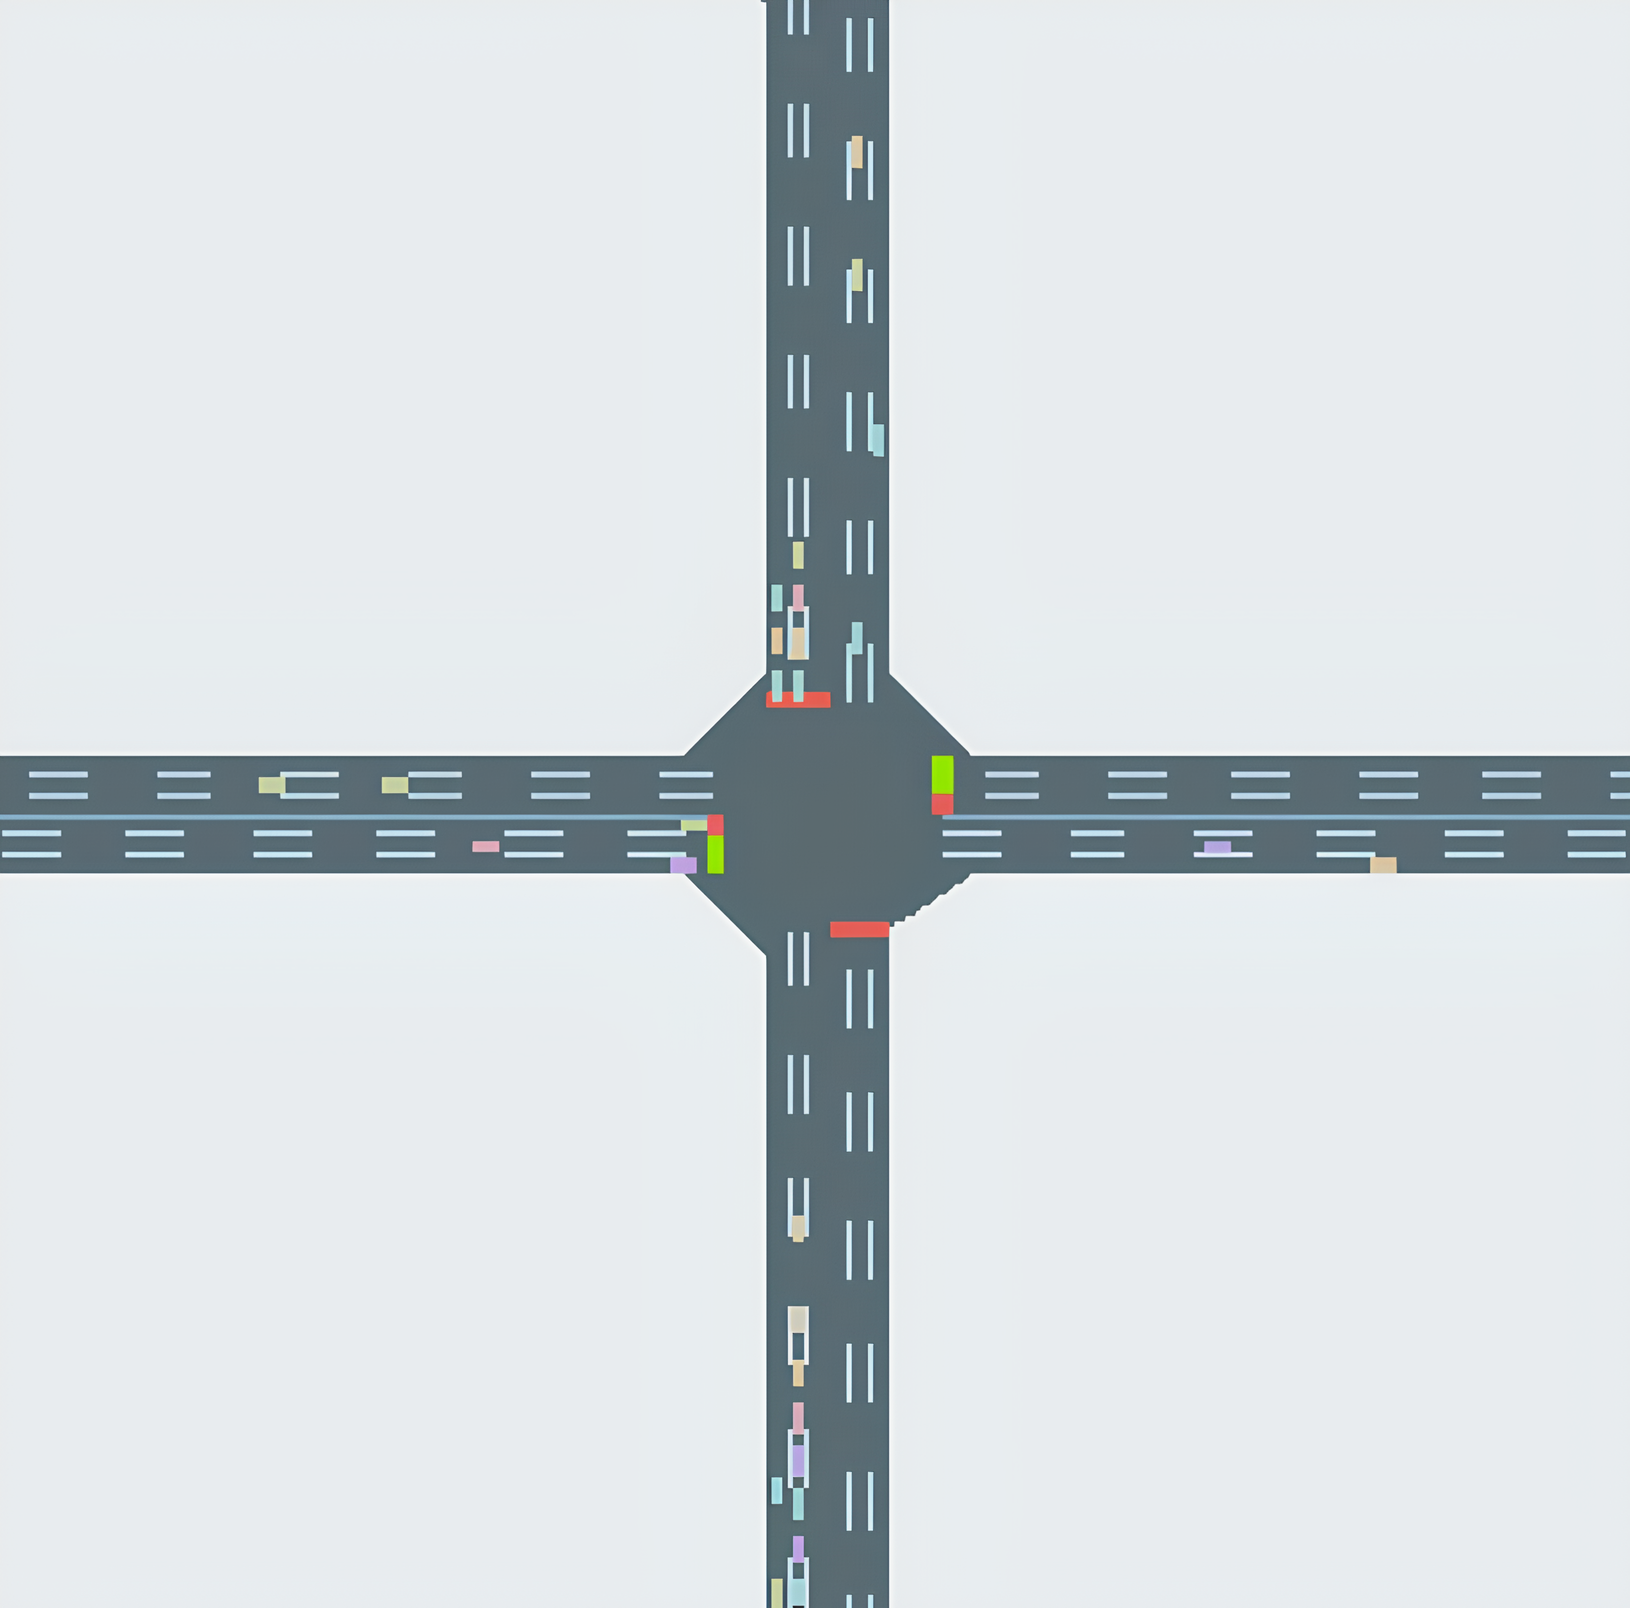
\includegraphics[width=0.7\textwidth]{screenshot_cityflow.png}
  \caption{Rendering del visualizzatore di \textsc{CityFlow} per una singola
    intersezione a quattro vie: le indicazioni verde/rosso ai margini
    dell'incrocio mostrano i movimenti abilitati dalla fase corrente, i
    rettangoli colorati sulle corsie i veicoli in transito o in coda.}
  \label{fig:cityflow-screenshot}
\end{figure}

\subsection{Struttura della rete e mappatura delle fasi}

La topologia della rete è codificata in un file di configurazione (\emph{roadnet}),
che definisce l'insieme delle intersezioni (nodi) e dei segmenti stradali (archi) con le relative molteplicità di corsia.
Per ogni intersezione il \emph{roadnet} elenca le fasi semaforiche disponibili, ciascuna definita
come l'insieme dei movimenti (coppie corsia di origine e di destinazione) abilitati in quella fase.
L'azione dell'agente si riduce pertanto alla selezione dell'indice corrispondente alla fase da attivare.
Ogni intersezione di questo lavoro modella 12 corsie in ingresso
(quattro direzioni cardinali, tre corsie ciascuna: sinistra, diritto, destra) e
8 fasi semaforiche selezionabili.
La tabella ~\ref{tab:fasi} riporta la mappatura di tali fasi, adottando la
nomenclatura N/S/E/W (\emph{North/South/East/West}) e T/L (\emph{Through}, diritto, e \emph{Left}, sinistra).

\begin{table}[htbp]
  \centering
  \small
  \begin{tabular}{@{}clp{7.5cm}@{}}
    \toprule
    Fase & Nome & Movimenti abilitati                      \\
    \midrule
    0    & NTST & Nord diritto+destra, Sud diritto+destra  \\
    1    & NLSL & Nord sinistra, Sud sinistra              \\
    2    & NTNL & Nord sinistra+diritto+destra             \\
    3    & STSL & Sud sinistra+diritto+destra              \\
    4    & WTET & Ovest diritto+destra, Est diritto+destra \\
    5    & WLEL & Ovest sinistra, Est sinistra             \\
    6    & ETEL & Est sinistra+diritto+destra              \\
    7    & WTWL & Ovest sinistra+diritto+destra            \\
    \bottomrule
  \end{tabular}
  \caption{Le 8 fasi semaforiche e i movimenti che ciascuna abilita.}
  \label{tab:fasi}
\end{table}

\begin{figure}[htbp]
  \centering
  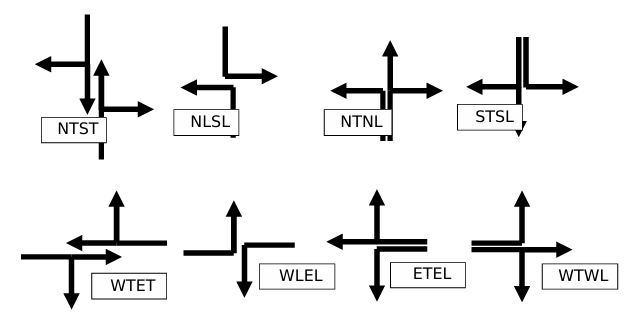
\includegraphics[width=0.85\textwidth]{fasi_semaforiche.png}
  \caption{Rappresentazione grafica delle 8 fasi di Tabella~\ref{tab:fasi}:
    le frecce indicano i movimenti abilitati da ciascuna fase.}
  \label{fig:fasi}
\end{figure}

Il paper originale permette ai veicoli che svoltano a destra di muoversi liberamente, senza attendere il semaforo verde, a patto che non vi siano veicoli provenienti da altre direzioni.
Al fine di prevenire una qualunque possibile interferenza tra diversi flussi e garantire un controllo più rigoroso, si è deciso di non adottare questo comportamento, permettendo la svolta a destra solo quando esplicitamente autorizzata dalla fase semaforica.
L'insieme delle fasi sopra riportate rappresenta una configurazione tale da sfruttare al massimo lo spazio delle direzioni possibili,
evitando al contempo conflitti tra le traiettorie dei veicoli.

\subsection{Gestione dell'interverde}

L'interverde è il periodo di tempo che intercorre tra la fine del verde di una fase semaforica
e l'inizio del verde di quella successiva.
Il suo scopo è quello di garantire la sicurezza stradale, permettendo ai veicoli che si trovano nell'intersezione di
sgombrarla prima che venga attivata la fase successiva.
Il motore di simulazione \textsc{CityFlow} non modella nativamente tale fase transitoria, nello specifico, non gestisce i semafori gialli e il conseguente passaggio sicuro tra due fasi consecutive;
dunque l'interverde deve essere costruito esplicitamente.
In questo lavoro, l'intervallo decisionale dell'agente (lo \emph{step} di simulazione) ha una durata complessiva $\Delta t_{\text{step}} = 15 \text{ s}$ simulati,
idealmente ripartita in tre sotto-fasi:
verde ($\Delta t_{\text{green}} = 10 \text{ s}$), giallo ($\Delta t_{\text{yellow}} = 3 \text{ s}$) e "tutto-rosso" ($\Delta t_{\text{red}} = 2 \text{ s}$).
Per il limite di \textsc{CityFlow} sopra descritto e in questo studio accettato come compromesso, l'ambiente assimila il giallo al verde senza imporre modelli di decelerazione specifici,
mantenendo pertanto i movimenti autorizzati dalla policy per una durata totale di  $\Delta t_{\text{green}}+\Delta t_{\text{yellow}} = 13 \text{ s}$ consecutivi.
Al termine di questa finestra temporale, viene eseguita per $\Delta t_{\text{red}} = 2 \text{ s}$ una fase che non è presente tra le azioni selezionabili dal modello,
ovvero il semaforo rosso in contemporanea su tutte le corsie.
Questo intervallo di guardia è necessario per garantire lo svuotamento dell'intersezione prima del cambio di fase, così da prevenire collisioni.
A questo punto lo step giunge al termine e il modello formula una nuova decisione, scegliendo quale delle 8 fasi implementare nel ciclo successivo.

È importante sottolineare che questa accortezza riduce di fatto il tempo effettivo utile di decisione del singolo agente di controllo semaforico, in quanto due dei quindici secondi di ogni step sono
dedicati alla fase "tutto-rosso" e quindi da considerarsi tempo morto (rappresentando circa il 13\% del tempo totale).

\subsection{Dataset e generazione parametrica}
\label{subsec:dataset}

Ogni roadnet e ogni flusso di traffico usato in questo lavoro è generato
parametricamente e in modo interamente deterministico da uno script dedicato,
senza alcun campionamento empirico.
Questo approccio consente di avere un pieno controllo sulle variabili operative come la
struttura della rete, la densità veicolare e presenza di arterie principali, oltre a
garantire l'esatta riproducibilità degli scenari di simulazione, un requisito metodologico fondamentale
per un equo confronto tra modelli di controllo semaforico.

\paragraph{Topologie e spaziature.}
L'ambiente di simulazione implementa tre topologie a griglia regolare di dimensioni $4\times4$ (16 intersezioni),
$5\times5$ (25 intersezioni) e $6\times6$ (36 intersezioni), impiegate per l'addestramento e per valutare la capacità di generalizzazione
dei modelli rispetto alla scala spaziale.

Un obiettivo centrale di questo lavoro consiste nell'indagare le capacità di coordinamento
implicito apprese dalle diverse policy di controllo. In quest'ottica, assume particolare
rilevanza la comparsa spontanea della così detta onda verde, uno standard strutturale nell'ingegneria del traffico contemporanea.
La spaziatura tra incroci è pertanto di due tipi: calibrata per l'onda verde e non calibrata.
In assenza di offset temporali, in quanto le transizioni di fase sono sincrone per tutti i nodi della rete,
l'unico modo per ottenere un'onda verde, ovvero un flusso di veicoli che si propagano
attraverso la rete senza fermarsi ai semafori, è calibrare la distanza fisica tra
gli incroci sulla velocità di marcia e sulla durata del ciclo:
alla velocità di riferimento $v_{\mathrm{urb}} = 11.1 \text{ m/s}$,
in un ciclo di $\Delta t_{\text{step}} = 15 \text{ s}$ viene percorsa una distanza pari a $166.5 \text{ m}$.
Dunque la prima spaziatura proposta è proprio di questa misura, ma ne faremo
riferimento con l'etichetta "100m".
La spaziatura non calibrata invece è 100m più estesa e viene indicata con "200m".

Le roadnet non condividono tutte lo stesso ruolo. La griglia $4\times4$ con spaziatura "100m" compare sia in training sia in test,
mentre le altre tre combinazioni topologia-spaziatura restano riservate esclusivamente al test e non vengono mai incontrate durante l'addestramento
(Tabella~\ref{tab:roadnet-uso}). Questa separazione serve a isolare due assi di generalizzazione: le griglie $5\times5$ e $6\times6$ misurano la tenuta
della policy su reti più estese di quella di addestramento, con più intersezioni da coordinare, mentre la spaziatura "200m" applicata alla griglia $4\times4$
misura la tenuta su una topologia mai vista con incroci più distanziati, priva della calibrazione per l'onda verde descritta sopra.

\begin{table}[htbp]
  \centering
  \small
  \begin{tabular}{@{}llc@{}}
    \toprule
    Griglia    & Spaziatura & Utilizzo                \\
    \midrule
    $4\times4$ & 100m       & Train, Validation, Test \\
    $4\times4$ & 200m       & Test                    \\
    $5\times5$ & 100m       & Test                    \\
    $6\times6$ & 100m       & Test                    \\
    \bottomrule
  \end{tabular}
  \caption{Utilizzo di ciascuna combinazione topologia-spaziatura. Il dettaglio del confine tra training e validazione sulla griglia $4\times4$ a 100m è in Tabella~\ref{tab:split}.}
  \label{tab:roadnet-uso}
\end{table}

\begin{figure}[htbp]
  \centering
  \begin{subfigure}[t]{0.48\textwidth}
    \centering
    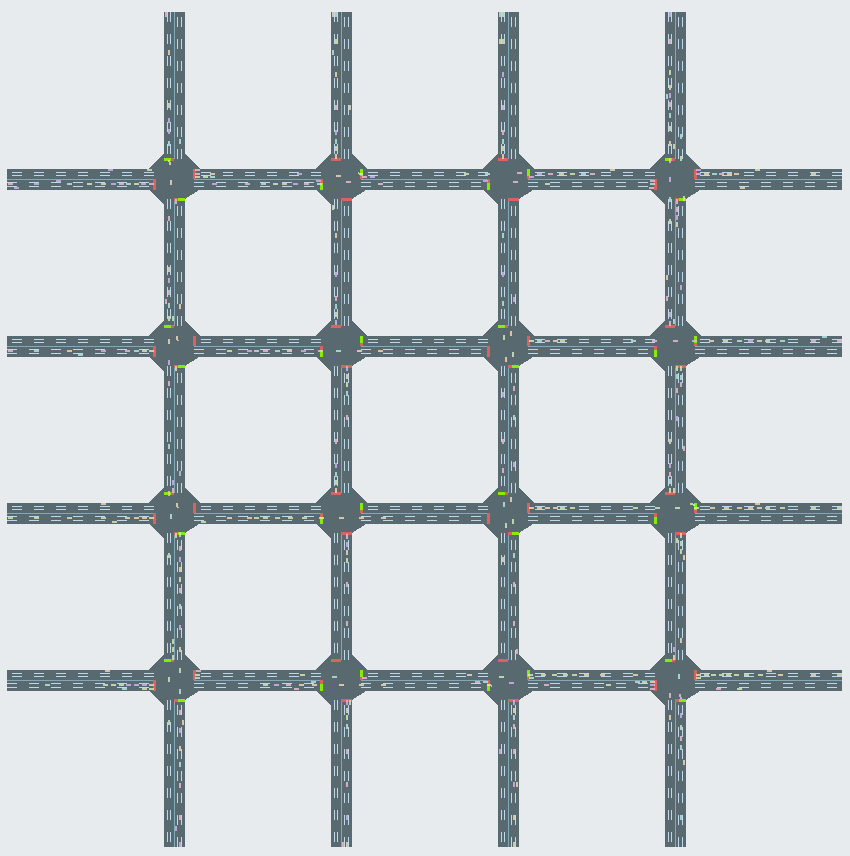
\includegraphics[width=\linewidth]{rete4x4.png}
    \caption{$4\times4$, 100m}
  \end{subfigure}
  \hfill
  \begin{subfigure}[t]{0.48\textwidth}
    \centering
    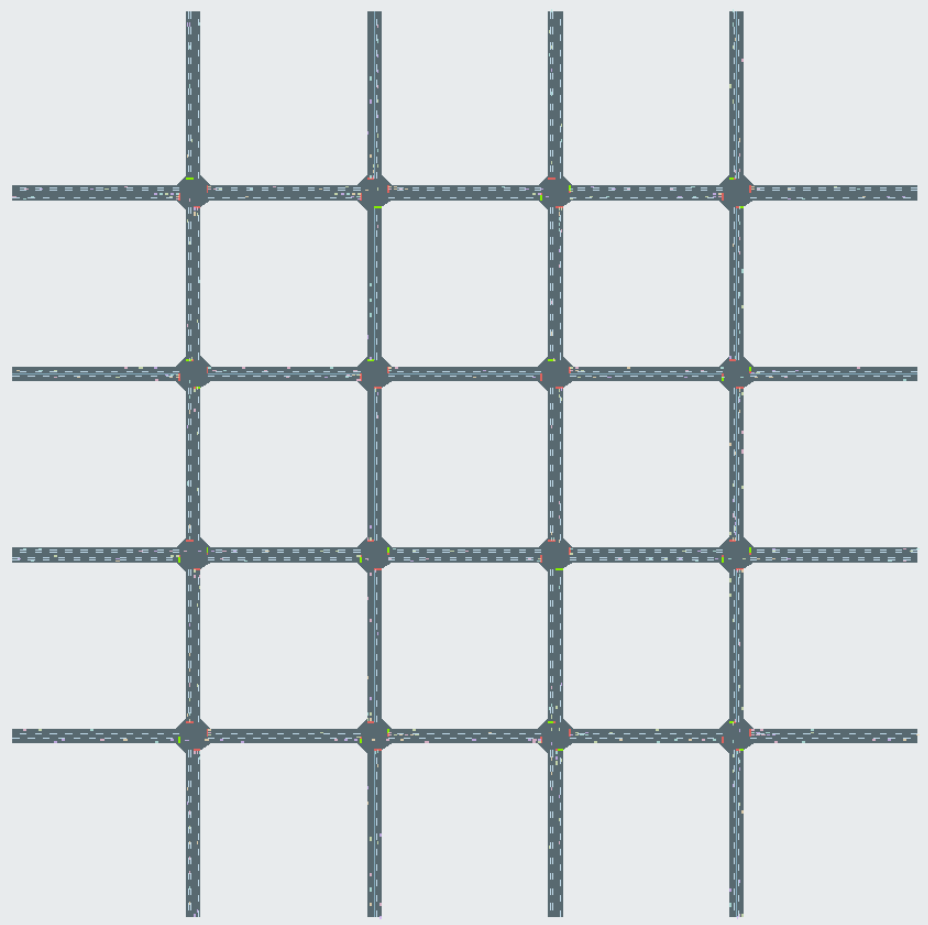
\includegraphics[width=\linewidth]{rete4x4_200m.png}
    \caption{$4\times4$, 200m}
  \end{subfigure}
  \par\bigskip
  \begin{subfigure}[t]{0.48\textwidth}
    \centering
    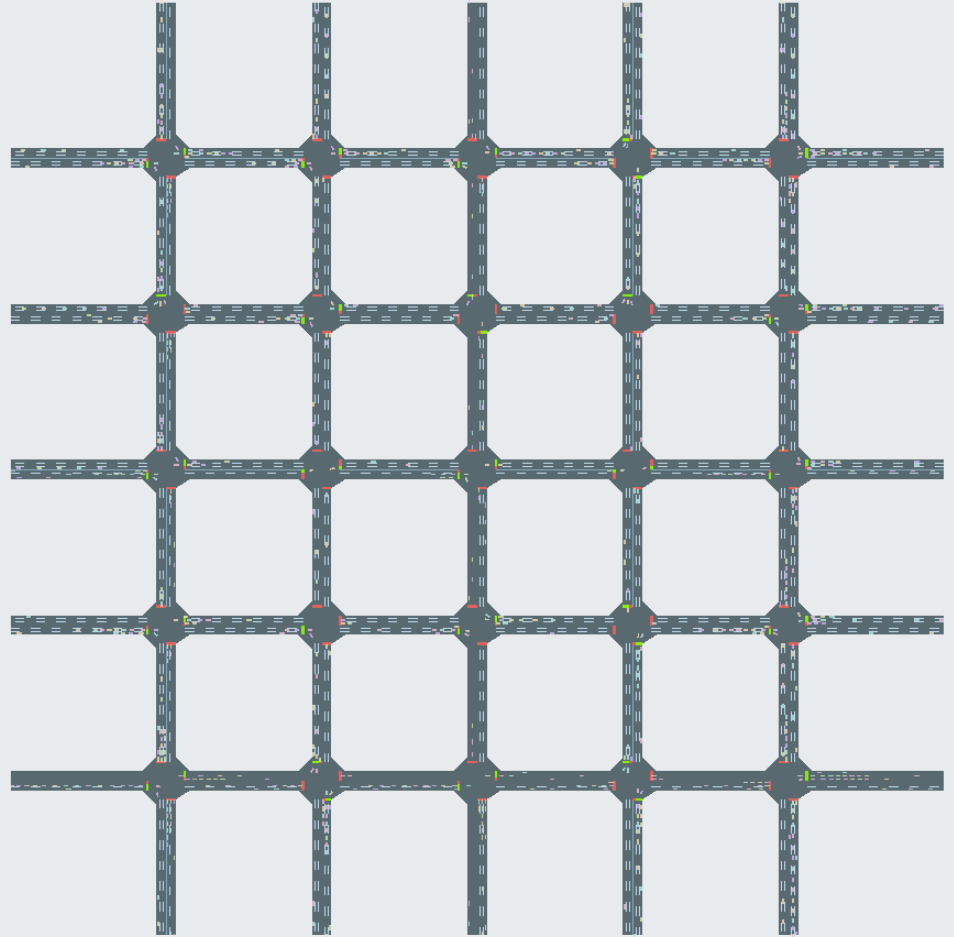
\includegraphics[width=\linewidth]{rete5x5.png}
    \caption{$5\times5$, 100m}
  \end{subfigure}
  \hfill
  \begin{subfigure}[t]{0.48\textwidth}
    \centering
    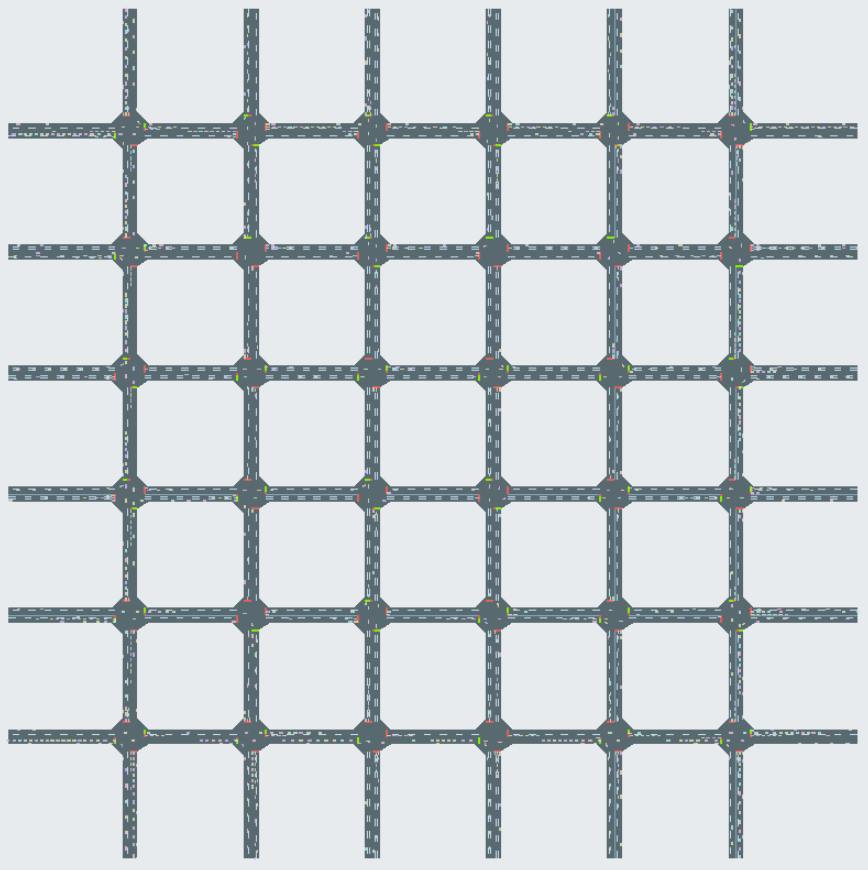
\includegraphics[width=\linewidth]{rete6x6.png}
    \caption{$6\times6$, 100m}
  \end{subfigure}
  \caption{Rendering nel visualizzatore di \textsc{CityFlow} delle quattro combinazioni topologia-spaziatura di Tabella~\ref{tab:roadnet-uso}.}
  \label{fig:roadnet-render}
\end{figure}

\paragraph{Percorsi veicolari.}
Il percorso di ciascun veicolo attraverso la rete non è fissato a priori, ma
generato casualmente per ciascun punto di ingresso sul perimetro della
griglia: a ogni incrocio attraversato, il percorso prosegue dritto con
probabilità $0.60$, svolta a destra con probabilità $0.30$ o svolta a
sinistra con probabilità $0.10$, finché non esce dai confini della rete o
non ripercorrerebbe un incrocio già attraversato (evitando così percorsi
ciclici). La probabilità complessiva di un percorso è il prodotto delle
probabilità delle singole scelte che lo compongono; il
numero di veicoli assegnato a ciascun percorso è proporzionale al suo peso relativo
sul totale dei percorsi generati da quel punto di ingresso, calibrato per
raggiungere il volume di traffico target di ciascuna fascia
(Tabella~\ref{tab:workday}).

\paragraph{Profili di traffico.}
Per ciascuna topologia sono stati generati tre profili di traffico:
un flusso a intensità costante (\emph{flat}),
un profilo a gradino (\emph{peak}, diviso in tre fasi temporali con un raddoppio del carico nel terzo centrale) e
un profilo dinamico (\emph{complete}) che simula il traffico di una giornata lavorativa (dettagliato nel seguito), impiegato esclusivamente in fase di addestramento.
Ogni episodio ha una durata di $T_{\text{max}} = 1800 \text{ s}$ simulati, corrispondenti a $1800 \text{ s} / \Delta t_{\text{step}} = 120$ cicli decisionali per agente.

I volumi dei veicoli immessi nella rete per ciascuna configurazione topologica sono stati determinati tramite una calibrazione empirica, così da garantire un livello
di saturazione comparabile tra reti di dimensioni diverse e quindi una difficoltà del task di controllo invariata rispetto la scala topologica.
In particolare la densità di ogni topologia è stata bilanciata affinché il \emph{trip completion} ottenuto dalla baseline \textsc{Max-Pressure} risultasse omogeneo ($90\%\text{--}94\%$).

\paragraph{Profilo di addestramento \emph{complete}.}
A differenza degli scenari di validazione e test, caratterizzati da densità costanti o a singolo picco,
il profilo di addestramento sintetizza l'evoluzione della domanda veicolare di un'intera giornata solare (24 ore) all'interno di un singolo episodio di $1800 \text{ s}$.
Come dettagliato nella Tabella~\ref{tab:workday}, il flusso è diviso in cinque fasce a intensità variabile:
due fasce a basso carico (assimilabili agli orari notturni),
due picchi di massima domanda (flussi di traffico di inizio e fine turno lavorativo) e
un intervallo di raccordo centrale a regime moderatamente sostenuto.
Questa marcata variazione di domanda veicolare all'interno di un singolo episodio è funzionale poiché costringe il modello ad adattare dinamicamente il piano di controllo,
senza convergere verso una policy specializzata soltanto su un unico flusso di traffico.

\begin{table}[htbp]
  \centering
  \small
  \begin{tabular}{@{}p{4.3cm}rrr@{}}
    \toprule
    Fascia     & Intervallo simulato & Step di decisione & Veicoli/secondo \\
    \midrule
    Flat basso & 0-525s              & 0-35              & 1.2             \\
    Peak basso & 525-675s            & 35-45             & 3.5             \\
    Flat alto  & 675-1200s           & 45-80             & 2.5             \\
    Peak alto  & 1200-1350s          & 80-90             & 4.2             \\
    Flat basso & 1350-1800s          & 90-120            & 1.2             \\
    \bottomrule
  \end{tabular}
  \caption{Le cinque fasce del profilo di addestramento \emph{complete}
    (totale: $\sim$ 4.700 veicoli).}
  \label{tab:workday}
\end{table}

\paragraph{Stocasticità e sbilanciamento direzionale.}
Per mitigare il rischio di \emph{overfitting} e garantire la robustezza del modello,
la generazione del profilo di addestramento integra due accorgimenti.

Innanzi tutto, considerata la natura deterministica di \textsc{CityFlow},
addestrare un modello su una singola configurazione esporrebbe l'agente all'apprendimento mnemonico di un'esatta sequenza di veicoli.
Per prevenire questa eventualità, si generano con diversi \emph{seed} tre profili di traffico differenti, in modo da perturbare
la distribuzione dei percorsi e gli istanti di immissione, pur mantenendo la medesima struttura generale descritta in Tabella~\ref{tab:workday};
tali varianti vengono quindi alternate ciclicamente durante l'addestramento.
Anche le configurazioni di validazione e test, su cui i modelli vengono valutati metodicamente, vengono generate con diversi \emph{seed},
così da ottenere statistiche più robuste e informative sui risultati conseguiti.

In secondo luogo, per mettere alla prova la capacità del modello di adattarsi a situazioni locali di traffico differenti,
è stata indotta un'asimmetria direzionale, designando una riga orizzontale della griglia come arteria principale (Est-Ovest),
dunque con densità di traffico maggiore delle strade trasversali, mantenendo comunque invariato il volume totale di veicoli.
Tale arteria viene posta su una riga diversa per ogni variante di addestramento, al fine di scongiurare l'ipotesi che le policy sviluppate siano dipendenti dalla posizione dell'incrocio,
mentre viene mantenuta fissa sulla stessa riga nelle configurazioni di validazione e di test, in modo da garantire la comparabilità dei risultati.

\paragraph{Training, validation e test.} La Tabella~\ref{tab:split}
raccoglie in un unico prospetto tutte le combinazioni di griglia, spaziatura
e profilo di traffico introdotte in questo lavoro, con il relativo utilizzo
nella pipeline sperimentale; le varianti seed di validazione e test sono
omesse, poiché non introducono combinazioni distinte da quelle elencate.
In tutto possiamo contare 11 configurazioni: 3 di training, 1 di validation e 7 di test.

\begin{table}[htbp]
  \centering
  \footnotesize
  \begin{tabular}{@{}lllll@{}}
    \toprule
    Griglia    & Spaziatura & Profilo di traffico       & Utilizzo    & Configurazione                          \\
    \midrule
    $4\times4$ & 100m       & Complete (arteria riga 0) & Train, Test & \texttt{config\_4x4\_100m\_train1}      \\
    $4\times4$ & 100m       & Complete (arteria riga 1) & Train, Test & \texttt{config\_4x4\_100m\_train2}      \\
    $4\times4$ & 100m       & Complete (arteria riga 2) & Train, Test & \texttt{config\_4x4\_100m\_train3}      \\
    $4\times4$ & 100m       & Flat                      & Validation  & \texttt{config\_4x4\_100m\_6k\_flat}    \\
    $4\times4$ & 100m       & Peak                      & Test        & \texttt{config\_4x4\_100m\_6k\_peak}    \\
    $4\times4$ & 200m       & Flat                      & Test        & \texttt{config\_4x4\_200m\_6k\_flat}    \\
    $4\times4$ & 200m       & Peak                      & Test        & \texttt{config\_4x4\_200m\_6k\_peak}    \\
    $5\times5$ & 100m       & Flat                      & Test        & \texttt{config\_5x5\_100m\_9.4k\_flat}  \\
    $5\times5$ & 100m       & Peak                      & Test        & \texttt{config\_5x5\_100m\_9.4k\_peak}  \\
    $6\times6$ & 100m       & Flat                      & Test        & \texttt{config\_6x6\_100m\_11.5k\_flat} \\
    $6\times6$ & 100m       & Peak                      & Test        & \texttt{config\_6x6\_100m\_11.5k\_peak} \\
    \bottomrule
  \end{tabular}
  \caption{Tutte le combinazioni di griglia, spaziatura e profilo di traffico impiegate in questo lavoro, a meno delle varianti seed di validazione e test, con il relativo utilizzo e il nome del file di configurazione corrispondente.}
  \label{tab:split}
\end{table}

\subsection{Assunzioni e limiti del modello di simulazione}
Si esplicitano di seguito le semplificazioni strutturali adottate in fase di simulazione, finalizzate a ridurre la complessità computazionale e a rendere il problema trattabile:
\begin{itemize}
  \item \textbf{Fasi transitorie:} Come precedentemente illustrato, l'intervallo semaforico di giallo è assimilato cinematicamente a un prolungamento del verde.
        La prevenzione dei conflitti è affidata unicamente alla fase di "tutto-rosso".
  \item \textbf{Omogeneità topologica:} L'analisi è confinata a topologie a griglia regolare, con incroci ortogonali e segmenti stradali di lunghezza uniforme.
        Tale astrazione permette di isolare l'impatto della sola scala dimensionale sulle prestazioni di generalizzazione, rimuovendo le distorsioni causate dalle irregolarità geometriche tipiche delle reti urbane reali.
  \item \textbf{Flusso unimodale e omogeneo:} La simulazione modella esclusivamente il traffico veicolare privato. Non sono previsti pedoni, ciclisti, trasporti pubblici o mezzi di soccorso.
        Inoltre, il flusso è perfettamente omogeneo: ogni veicolo condivide i medesimi parametri cinematici (dimensione, accelerazione massima, velocità massima).
  \item \textbf{Limiti di velocità uniformi:} Il limite di velocità $v_{\mathrm{urb}}=11.1$ m/s è una costante globale, identica per ogni corsia della rete e per ogni veicolo generato, dunque sono assenti gerarchie stradali diverse.
  \item \textbf{Omogeneità degli incroci:} Ogni intersezione è vincolata a una geometria a quattro vie provvista di 8 fasi semaforiche, escludendo di fatto incroci con un numero diverso di vie.
  \item \textbf{Assenza di \emph{lane-changing}:} Le corsie in approccio sono dedicate in modo esclusivo ai singoli movimenti (svolta a sinistra, dritto, svolta a destra).
        I veicoli vengono generati e si immettono automaticamente nella corsia compatibile con il loro percorso e il cambio di corsia (\emph{lane-changing}) è una dinamica che non è stata implementata.
  \item \textbf{Viabilità bidirezionale:} L'infrastruttura di rete è composta esclusivamente da strade a doppio senso di marcia.
        La modellazione di strade a senso unico, per quanto frequente nei contesti urbani, non rientra nell'insieme delle configurazioni generate.
\end{itemize}







\section{Baseline classiche}
\label{sec:baseline}

In questo capitolo vengono introdotte le due baseline classiche di riferimento nella letteratura del Traffic Signal Control: Fixed-Time e Max-Pressure.
Nello specifico, pur fondandosi su paradigmi di controllo opposti, l'uno statico e l'altro adattivo, entrambi gli approcci sono accomunati dal fatto di non richiedere alcuna fase di addestramento.
Proprio questa loro natura li rende i candidati ideali per essere confrontati con i modelli di Deep Reinforcement Learning.

\paragraph{Fixed-Time.}
Questo algoritmo cicla le fasi semaforiche di un incrocio in ordine fisso,
cambiando fase a ogni step di decisione. Fixed-Time non osserva mai lo stato
della rete, non ha alcun parametro da configurare oltre all'ordine del
ciclo e non richiede training.
È un approccio estremamente semplice da implementare ed è la spina dorsale della stragrande maggioranza dei sistemi semaforici a livello globale,
dove le uniche modifiche proposte riguardano l'ordine delle fasi semaforiche (in cui una fase può essere ripetuta più di una volta per ciclo),
la durata di ciascuna fase e una complessiva estensione o restrizione del ciclo semaforico in base all'orario giornaliero.
Poiché non richiede sensori stradali in tempo reale né potenza computazionale per calcolare le decisioni, esso risulta essere estremamente economico in termine di strumentazione.
Gli svantaggi principali riguardano la sua rigidità e la sua intrinseca incapacità di adattarsi alle fluttuazioni improvvise del traffico,
delle caratteristiche che possono risultare fatali per il traffico in caso di eventi imprevisti.

\paragraph{Max-Pressure.}
L'algoritmo Max-Pressure proposto da \citep{varaiya2013maxpressure} rappresenta un sistema di controllo reattivo che garantisce matematicamente
il massimo throughput (capacità di smaltimento dei veicoli) della rete stradale senza alcuna necessità di training, partendo dalla teorica assunzione che le strade abbiano capacità infinita.
Questo straordinario risultato, pur non potendo essere traslato integralmente in scenari reali dove non è rara la possibilità di una completa
saturazione di una via, fa affidamento solamente a dati raccolti ad ogni istante decisionale nelle corsie adiacenti all'incrocio e a un principio di base: massimizzare la pressione di ciascuna fase semaforica.
Nel dettaglio questo principio prevede che, dato un incrocio $i$ e una fase semaforica $\phi$, la pressione della fase sia definita come la somma,
su tutti i movimenti (coppia corsia di ingresso/corsia di uscita) abilitati da $\phi$, della differenza tra il numero di veicoli in attesa (i.e. non in movimento) e il numero di veicoli in uscita,
contati sull'intera corsia; formalmente:
\begin{equation}
  P(i,\phi) = \sum_{(\ell_{\mathrm{in}}, \ell_{\mathrm{out}}) \,\in\, \mathrm{movimenti}(\phi)} \Big( n(\ell_{\mathrm{in}}) - n(\ell_{\mathrm{out}}) \Big)
  \label{eq:maxpressure}
\end{equation}
dove $n(\ell)$ indica il numero di veicoli nella corsia $\ell$, $\ell_{\mathrm{in}}$ una corsia in ingresso e $\ell_{\mathrm{out}}$ una corsia in uscita,
$\mathrm{movimenti}(\phi)$ i movimenti abilitati dalla fase $\phi$.
Max-Pressure, a ogni step di decisione, calcola la pressione di tutte le fasi e seleziona quella a pressione massima, ovvero:
\[ \phi^*(i) = \operatorname*{argmax}_\phi P(i,\phi) .\]
Uno svantaggio di questo algoritmo è dato dalla richiesta di sensoristica per monitorare le corsie per la loro interezza;
inoltre non è previsto alcun vincolo sulle azioni consecutive, ciò implica che in linea di principio la stessa fase può essere selezionata per un numero indefinito
di volte.
Ma il problema principale di questo approccio consiste nell'assenza di garanzie di equità: infatti, in presenza di un forte afflusso di traffico su un certo insieme di corsie,
la pressione maggiore potrebbe trovarsi sempre sulle fasi che coinvolgono tali vie, rendendo impossibile alle altre fasi la possibilità di essere selezionate,
con conseguenti tempi di attesa eccessivi per i veicoli che si trovano sulle vie caratterizzate da un minore afflusso veicolare.





\section{Architettura MetaSTGAT}
\label{sec:architettura}

Questo capitolo introduce il modello principale attorno a cui si sviluppa l'intero lavoro, sulla base dell'arichitettura originale proposta da \citep{wang2022metastgat}: MetaSTGAT.
La scelta di replicare e modificare tale modello è stata dettata dalla volontà di creare un sistema che potesse avere le caratteristiche ritenute necessarie
per proporre una soluzione accettabile al problema del Traffic Signal Control secondo dei termini specifici di questo lavoro di tesi:
ottenere un modello in grado di coordinare in modo efficace gli incroci di una rete stradale, così da minimizzare i tempi di percorrenza medi dei veicoli e
garantire, per quanto possibile, un certo grado di equità tra i vari flussi di veicoli.
A differenza di Fixed-Time, MetaSTGAT è un modello sensibile allo stato della rete per quanto riguarda la scelta delle fasi, e,
diversamente da Max-Pressure, cerca un compromesso tra \emph{throughput} (la capacità di smaltimento dei veicoli) e \emph{starvation} (l'eccessivo tempo di attesa dei veicoli);
tutto questo a costo di una richiesta di informazioni più dettagliata da raccogliere ad ogni istante decisionale (§\ref{sec:formalizzazione}) e a costo di una fase di addestramento.

L'architettura di questo modello di reinforcement learning si articola nei seguenti componenti, organizzati in una pipeline
che elabora lo stato di ogni intersezione ($s_i^t$) portandolo ad una rappresentazione compatta,
utilizzata per produrre i Q-value (ovvero una stima della ricompensa attesa per ciascuna azione):
\begin{itemize}
  \item un encoder di stato duale
  \item una cella ricorrente (LSTM)
  \item due istanze di un layer di \emph{graph attention} (GAT)
  \item due moduli di meta-learning, spaziale e temporale
  \item una layer lineare per calcolare i Q-value.
\end{itemize}

Analizzeremo qui ciascun componente citato, soffermandoci sulla ragione che ha condotto all'introduzione di tali elementi e
sulle modifiche apportate all'architettura originale.
Prima di introdurre la generalizzazione "meta",
ci concentreremo sulla presentazione dell'architettura STGAT,
ovvero la versione standard del modello priva del meccanismo di meta-apprendimento.
La Figura~\ref{fig:stgat-architettura} anticipa in forma schematica la pipeline appena
elencata, utile come riferimento visivo durante la lettura dei paragrafi che seguono.

\begin{figure}[htbp]
  \centering
  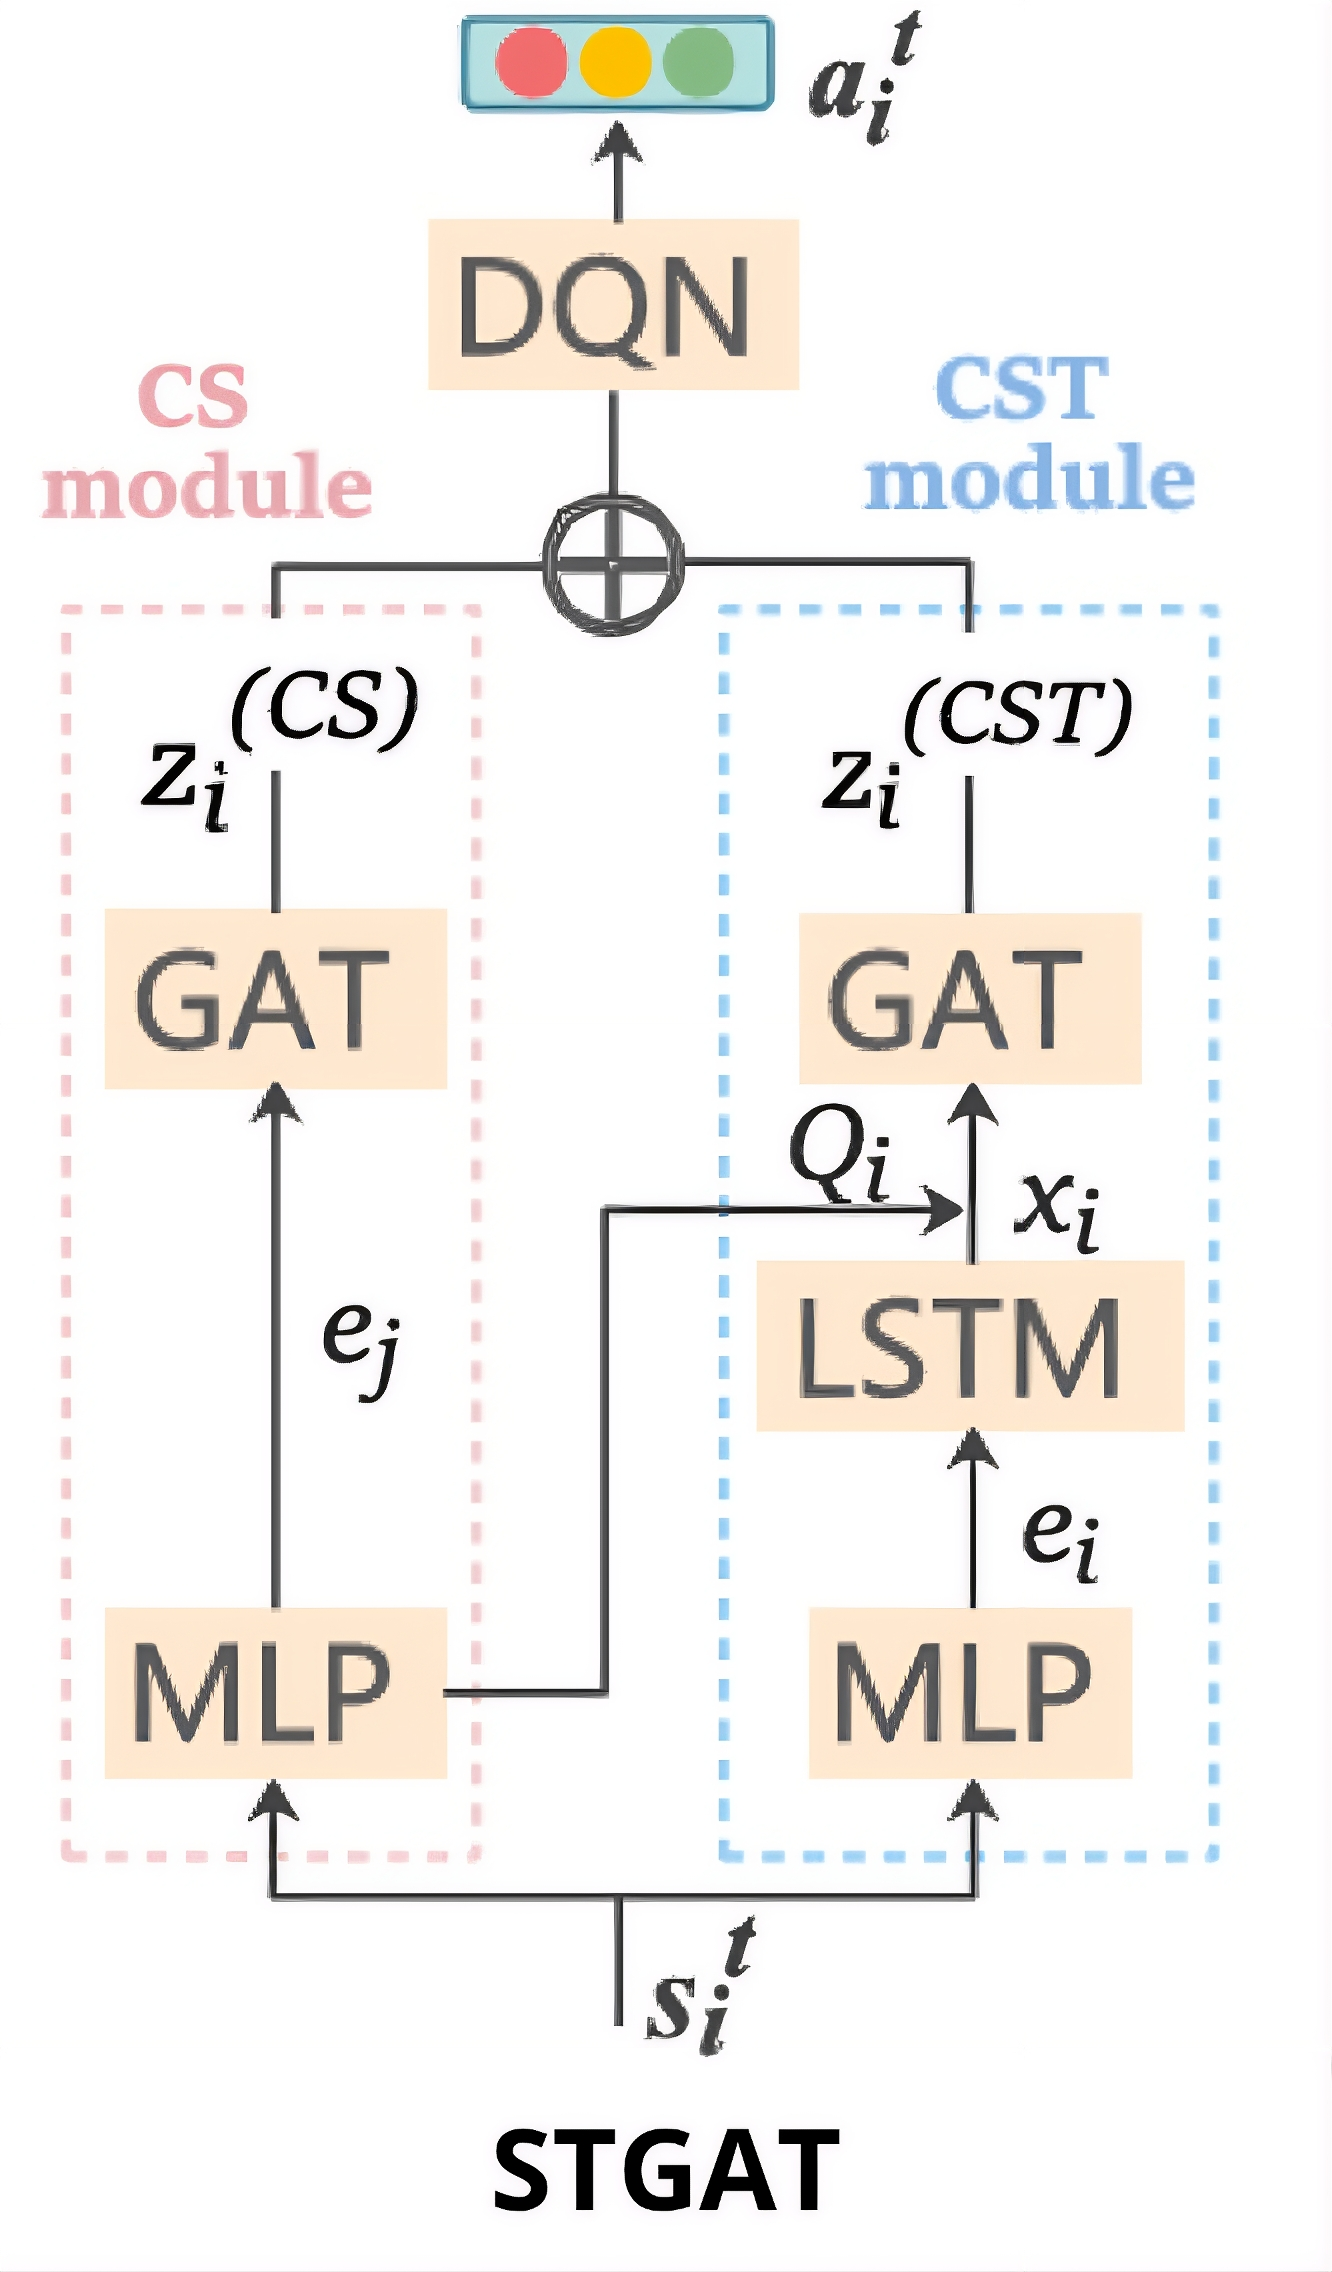
\includegraphics[width=0.55\textwidth]{architettura_stgat.png}
  \caption{Schema a blocchi dell'architettura STGAT: dallo stato dell'intersezione
    $s_i^t$, attraverso l'encoder duale (MLP) e i moduli CS e CST (GAT e LSTM a
    pesi condivisi), fino all'azione $a_i^t$ scelta dal DQN. Adattato da
    \citet{wang2022metastgat}.}
  \label{fig:stgat-architettura}
\end{figure}

\subsection{State Encoder duale}
\label{subsec:state-encoder}

Lo stato $s_i^t \in \mathbb{R}^{d_0}$ ($d_0=32$ o $20$, §\ref{sec:formalizzazione}) di un incrocio $i$ al tempo $t$
attraversa due Multilayer Perceptron (MLP) a due strati con la stessa architettura ma pesi e
inizializzazioni indipendenti:
\begin{align}
  e_i^t & = \mathrm{MLP_t}(s_i^t) = \sigma\big(W_{21}\,\sigma(W_{11} s_i^t + b_{11}) + b_{21}\big) \in \mathbb{R}^{d_1} \\
  e_j^t & = \mathrm{MLP_s}(s_i^t) = \sigma\big(W_{22}\,\sigma(W_{12} s_j^t + b_{12}) + b_{22}\big) \in \mathbb{R}^{d_1}
\end{align}
dove $d_1$ viene fissato a $64$, $W_{11},W_{12}\in\mathbb{R}^{d_0\times d_1}$ e $W_{21},W_{22}\in\mathbb{R}^{d_1\times d_1}$ sono i pesi,
$b_{11}, b_{21}, b_{12}, b_{22}\in\mathbb{R}^{d_1}$ i bias e
$\sigma$ la funzione di attivazione ReLU.

Il vettore $e_i^t = \mathrm{MLP_t}(s_i^t)$ verrà usato come input nella LSTM e veicolerà le caratteristiche temporali dello stato,
mentre $e_j^t = \mathrm{MLP_s}(s_i^t)$ verrà usato come input nelle GAT, catturando le caratteristiche spaziali dello stesso.


\subsection{Modulo spazio-temporale corrente (CST)}
\label{subsec:cst-module}

Nel momento di una decisione, un conteggio istantaneo dei veicoli, da solo, non distingue una coda che si
sta formando da una che si sta esaurendo. Due situazioni che possono
richiedere una fase diversa appaiono dunque identiche a un modello privo
di memoria. Il primo dei due moduli di STGAT viene introdotto per questo motivo:
combina l'informazione temporale accumulata da un'intersezione con
l'informazione spaziale corrente di sé stessa e dei suoi vicini, così che la scelta dell'azione
possa tenere conto di come il traffico più ravvicinato si sta
evolvendo, non solo di come si presenta localmente nell'istante attuale.
Altri lavori in materia cercano di applicare lo stesso concetto proponendo delle Spatio-Temporal Graph Neural Networks (STGNN) con una struttura simile a quella che introdurremo qui sotto,
ma in questi modelli le informazioni spaziali e temporali sono semplicemente combinate in un unico embedding, oppure usate separatamente.
Con il presente modulo si cerca di ovviare a questa limitazione intrecciando le informazioni spaziali e temporali in modo più elaborato.

Il ramo temporale dell'encoder $e_i^t$ (§\ref{subsec:state-encoder})
attraversa anzitutto una cella LSTM con pesi condivisi da ogni nodo della rete:
\begin{equation}
  \begin{bmatrix} f_i^t \\ \iota_i^t \\ o_i^t \\ g_i^t \end{bmatrix} =
  \begin{bmatrix} \sigma \\ \sigma \\ \sigma \\ \tanh \end{bmatrix}
  \left(
  W_{\{f,\iota,o,g\}}^{\top} [\,e_i^t \,\|\, h_i^{t-1}\,] + b_{\{f,\iota,o,g\}}
  \right),
  \label{eq:stgat-lstm-gates}
\end{equation}
\[ c_i^t = f_i^t \odot c_i^{t-1} + \iota_i^t \odot g_i^t, \]
\[ x_i^t = h_i^t = o_i^t \odot \tanh(c_i^t); \]
in notazione compatta:
\begin{equation}
  \big(h_i^t,\, c_i^t\big) = \mathrm{LSTM}\big(e_i^t \,;\, h_i^{t-1},\, c_i^{t-1}\big).
  \label{eq:stgat-lstm-compact}
\end{equation}
Il vettore $x_i^t := h_i^t$ prodotto da questa cella rappresenta concettualmente un riassunto temporale dei flussi di traffico locali.

Lo stesso vettore, nel meccanismo di attenzione che segue, diventa l'informazione che i vicini dell'incrocio $i$ "leggono"
per decidere quanto pesare il contributo di $i$ nel proprio contesto locale. Questa trasmissione di informazione avviene
tramite l'applicazione di una Graph Attention Network (GAT) con una rappresentazione differente rispetto a
quella della GAT standard di \citet{velickovic2018gat} riportata nel Capitolo~\ref{cap:background}.
In tale GAT infatti ciascun nodo viene comparato con gli altri nodi secondo una stessa proiezione dell'embedding.
Nella struttura proposta invece, prendendo ispirazione da approcci di machine translation (\cite{vaswani2017attention}), i nodi si influenzano vicendevolmente secondo valori distinti: Query, Key e Value.
In particolare si scelgono come Query $Q=e_j^t$ (la codifica spaziale corrente del nodo ricevente) e come Key e Value $K=V=x_i^t$ (la memoria temporale di ciascun vicino).
L'idea alla base di questa scelta è il tentativo di arricchire le caratteristiche temporali correnti di ciascun nodo con la memoria temporale dei flussi dello stesso e dei nodi vicini.
Si precisa che nel caso di $H>1$ teste di attenzione, come in questo lavoro, i valori $Q,K,V$ non sono proiettati da matrici distinte per ciascuna testa, bensì
il vettore a $d_1$ componenti viene partizionato in $H$ segmenti contigui di dimensione $d_h = d_1/H$, e la testa $h$ opera sul solo blocco $Q_h(i) := Q(i)[h d_h : (h{+}1)d_h]$ (analogamente per $K_h(u)$, $V_h(u)$).
Le teste restano quindi distinte perché leggono porzioni diverse dello stesso embedding, non perché dispongano di proiezioni apprese proprie.

Formalmente, nel caso in esame, per ciascun nodo $i$ con vicinato $\mathcal{N}(i)$ (con $i\in \mathcal{N}(i)$) e $h$ una delle $H=4$ teste di dimensione $d_h = d_1/H = 16$, questo modulo di GAT viene descritto come segue:
\begin{equation}
  \varphi_h(i,u) = \frac{Q_h(i) \cdot K_h(u)}{\sqrt{d_h}} ,
  \label{eq:stgat-attn}
\end{equation}
\[ \alpha_h(i,u) = \frac{\exp(\varphi_h(i,u))}{\sum_{u' \in \mathcal{N}(i)} \exp(\varphi_h(i,u'))}, \]
\[ z_h(i) = \sum_{u \in \mathcal{N}(i)} \alpha_h(i,u)\, V_h(u) .\]

L'output finale di questo modulo spazio-temporale corrente sarà
\[ z_{\mathrm{CST}}(i) = [z_1(i) \| \dots \| z_H(i)] \in \mathbb{R}^{d_1}. \]
Auspicabilmente, in questo stato è racchiusa una sintesi delle dinamiche spaziali e temporali del traffico locale e degli incroci adiacenti.


\subsection{Modulo spaziale corrente (CS)}
\label{subsec:cs-module}

Il modulo spazio-temporale, filtrato dalla memoria della cella ricorrente,
può attenuare segnali che sono invece rilevanti nell'istante
presente; ad esempio un picco di traffico simultaneo su un intero asse
necessita di coordinamento spaziale puro, a prescindere dalla durata del picco stesso.
Questo secondo modulo, strutturalmente simile al primo,
elabora perciò la sola informazione spaziale corrente $e_j^t$, senza alcuna
componente di memoria.
Il vettore $e_j^t$ attraversa una GAT che opera secondo le stesse dinamiche descritte
nel paragrafo precedente, ma con l'assegnazione $Q=K=V=e_j^t$.
L'output finale del modulo spaziale corrente sarà
\[ z_{\mathrm{CS}}(i) = [z_1(i) \| \dots \| z_H(i)] \in \mathbb{R}^{d_1} ,\]
Tale rappresentazione del traffico permetterà al modello di focalizzarsi sulla coordinazione dei nodi rispetto alla sola fotografia presente della rete.

\subsection{Testa Q-value}
\label{subsec:q-head}

Le due uscite, $z_{\mathrm{CST}}(i)$ e $z_{\mathrm{CS}}(i)$, catturano
quindi aspetti complementari, l'uno informato dalla memoria temporale dei
vicini, l'altro dalla sola situazione presente. Tali vettori vengono infine concatenati e attraversano un singolo layer lineare per
produrre la stima del valore di ciascuna delle 8 azioni eseguibili all'incrocio $i$ e all'istante $t$:
\begin{equation}
  q(s_i^t, \cdot\,) = W_q\,[\,z_{\mathrm{CST}}(i) \,\|\, z_{\mathrm{CS}}(i)\,] + b_q \in \mathbb{R}^{8}
\end{equation}
dove $W_q \in \mathbb{R}^{8 \times 2 d_1}$ e $b_q \in \mathbb{R}^{8}$.

\subsection{Meta-knowledge learner}

I due moduli appena descritti, alla base della struttura STGAT, condividono gli stessi pesi
per ogni intersezione della rete, indipendentemente dal ruolo che occupa.
Ad esempio un incrocio periferico, uno pienamente interno alla rete stradale, o uno
attraversato da un'arteria a densità di traffico elevata
(§\ref{subsec:dataset}) applicano esattamente la stessa regola di coordinamento.
MetaSTGAT introduce un meccanismo di meta-apprendimento che condiziona
tale regola su un embedding di caratteristiche locali dell'incrocio,
cosicché i layer di GAT e di LSTM possano specializzarsi
rispetto alle condizioni osservate da ciascun nodo invece di applicare la stessa
funzione ovunque. L'idea alla base di questo meccanismo, condivisa da
entrambi i componenti "meta" che seguono, è illustrata in
Figura~\ref{fig:meta-learning-overview}: le meta-feature spaziali e
temporali, elaborate da un meta-learner dedicato, generano i pesi dei layer
di LSTM e GAT al posto di parametri fissi condivisi da ogni nodo.

\begin{figure}[htbp]
  \centering
  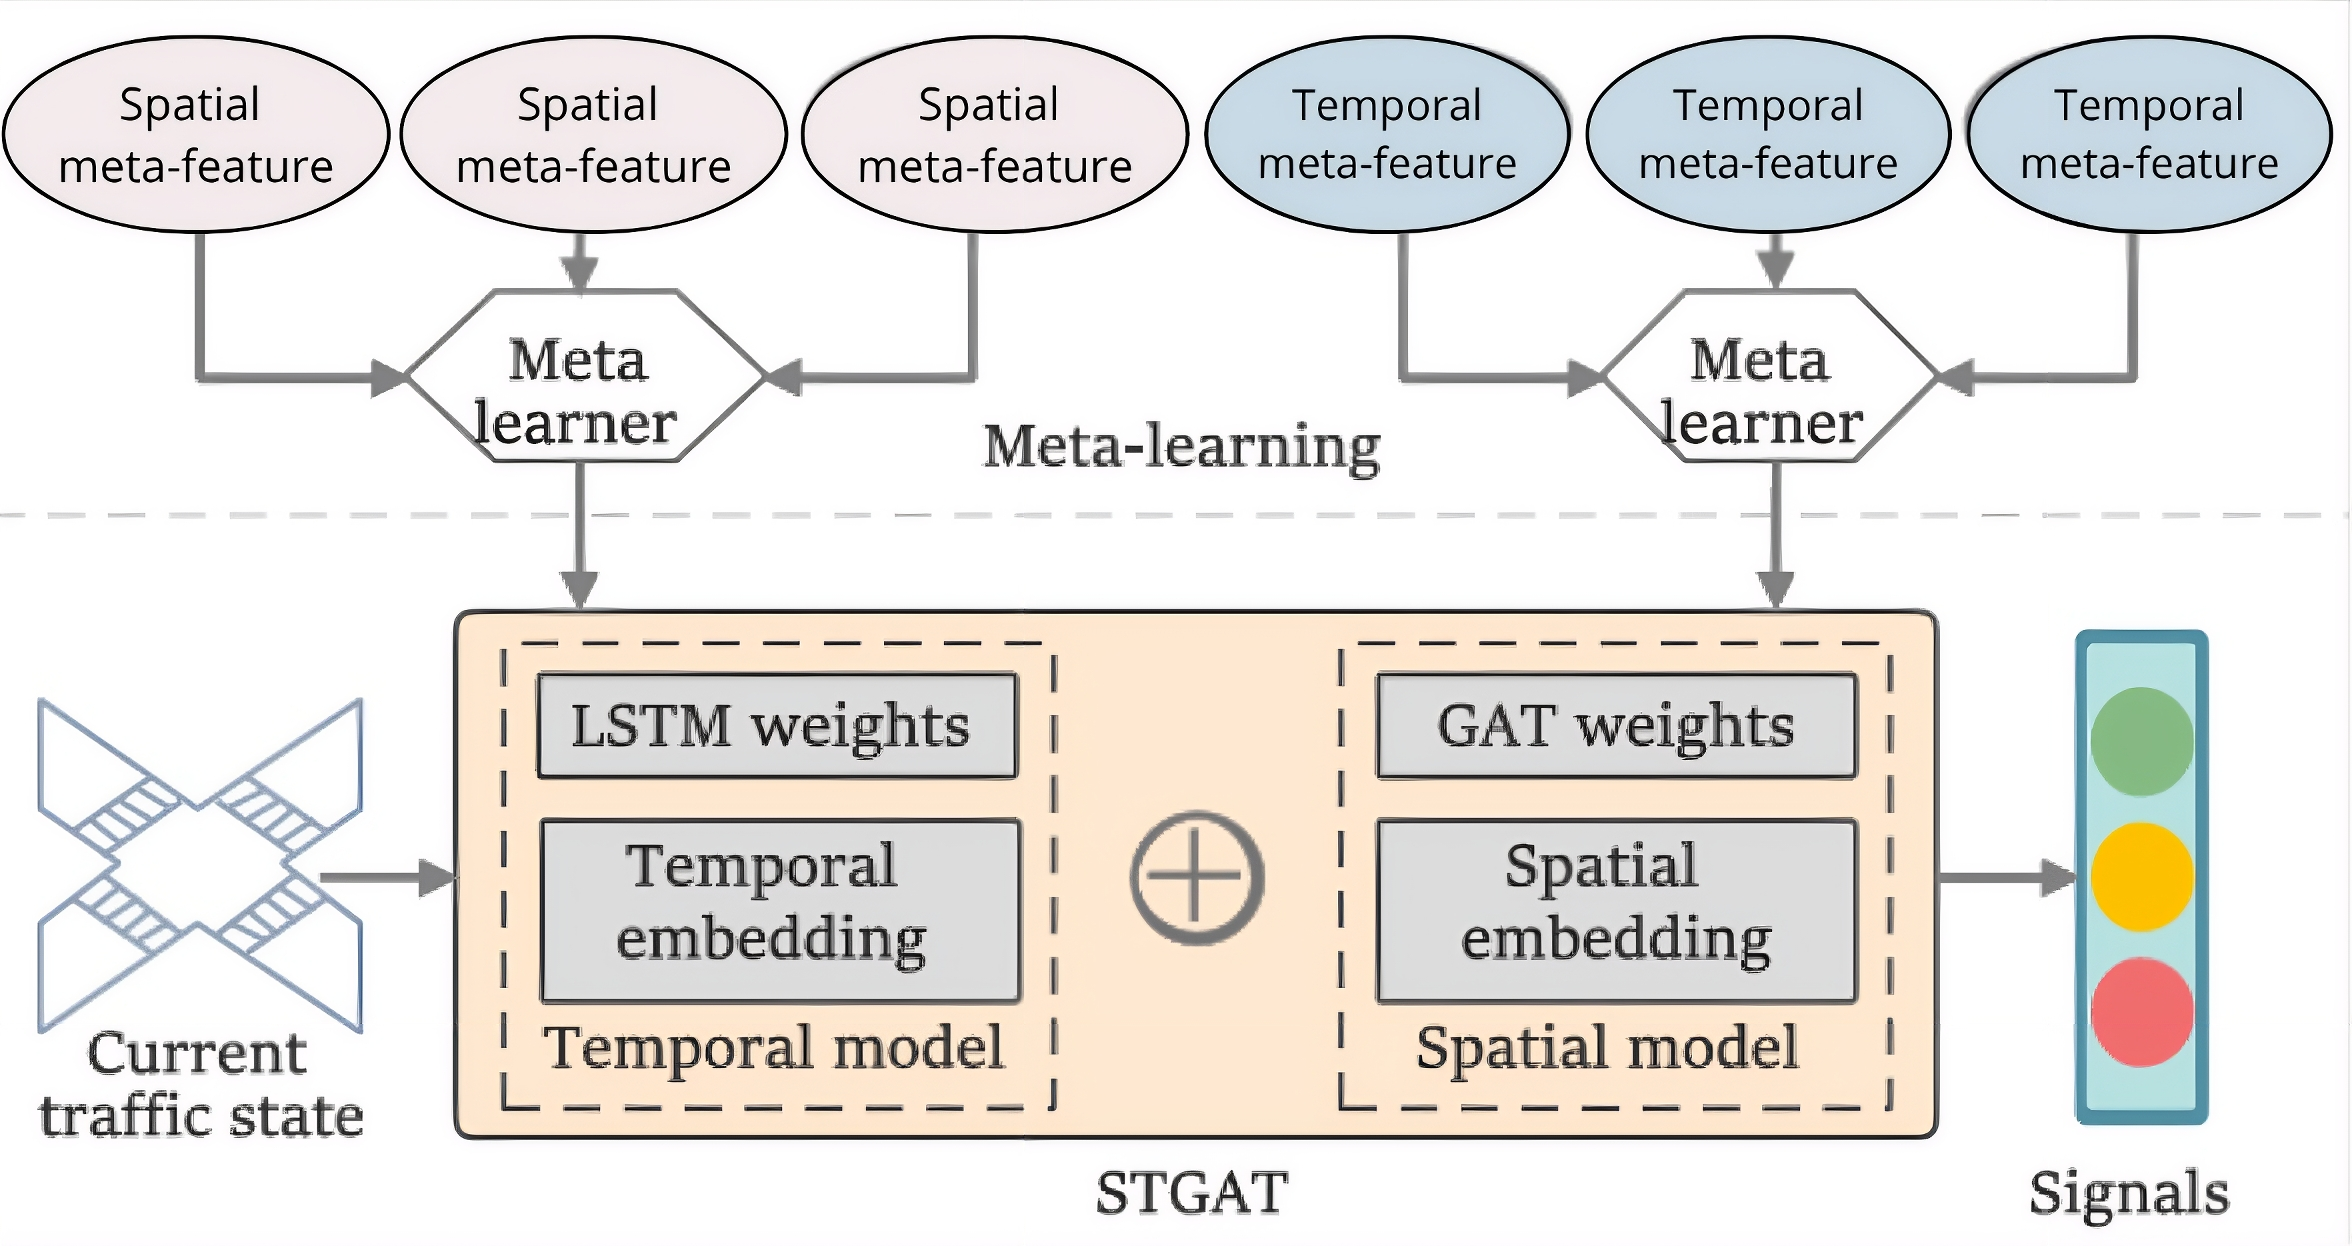
\includegraphics[width=0.75\textwidth]{meta_learning_overview.png}
  \caption{Principio del meta-apprendimento applicato da MetaSTGAT: le
    meta-feature spaziali e temporali condizionano, tramite un meta-learner
    dedicato, i pesi dei layer LSTM e GAT usati per elaborare lo stato corrente
    del traffico. Adattato da \citet{wang2022metastgat}.}
  \label{fig:meta-learning-overview}
\end{figure}

In particolare, due MLP a due strati, uno per l'aspetto spaziale e uno per quello temporale del
problema, apprendono un embedding di caratteristiche locali dell'intersezione (Spatial Meta-Knowledge, SMK; Temporal Meta-Knowledge, TMK)
a partire dalle meta-feature che descrivono il nodo ($x^{\mathrm{smk}}_i$ e $x^{\mathrm{tmk}}_i$):
\begin{align}
  \mathrm{SMK}(i) & = \mathrm{MLP}_{\mathrm{smk}}\big(x^{\mathrm{smk}}_i\big) \in \mathbb{R}^{64} \\
  \mathrm{TMK}(i) & = \mathrm{MLP}_{\mathrm{tmk}}\big(x^{\mathrm{tmk}}_i\big) \in \mathbb{R}^{64}
\end{align}
Come già accennato, tali valori verranno poi usati per generare i pesi di Meta-GAT e Meta-LSTM,
tramite dei MLP addizionali specializzati per ciascuno dei moduli, secondo quanto riporteremo in
(§\ref{subsec:meta-gat}) e (§\ref{subsec:meta-lstm}).
Il passaggio dalle meta-feature grezze ai due embedding $\mathrm{SMK}(i)$ e
$\mathrm{TMK}(i)$ è riassunto graficamente in Figura~\ref{fig:meta-knowledge-learner}.

\begin{figure}[htbp]
  \centering
  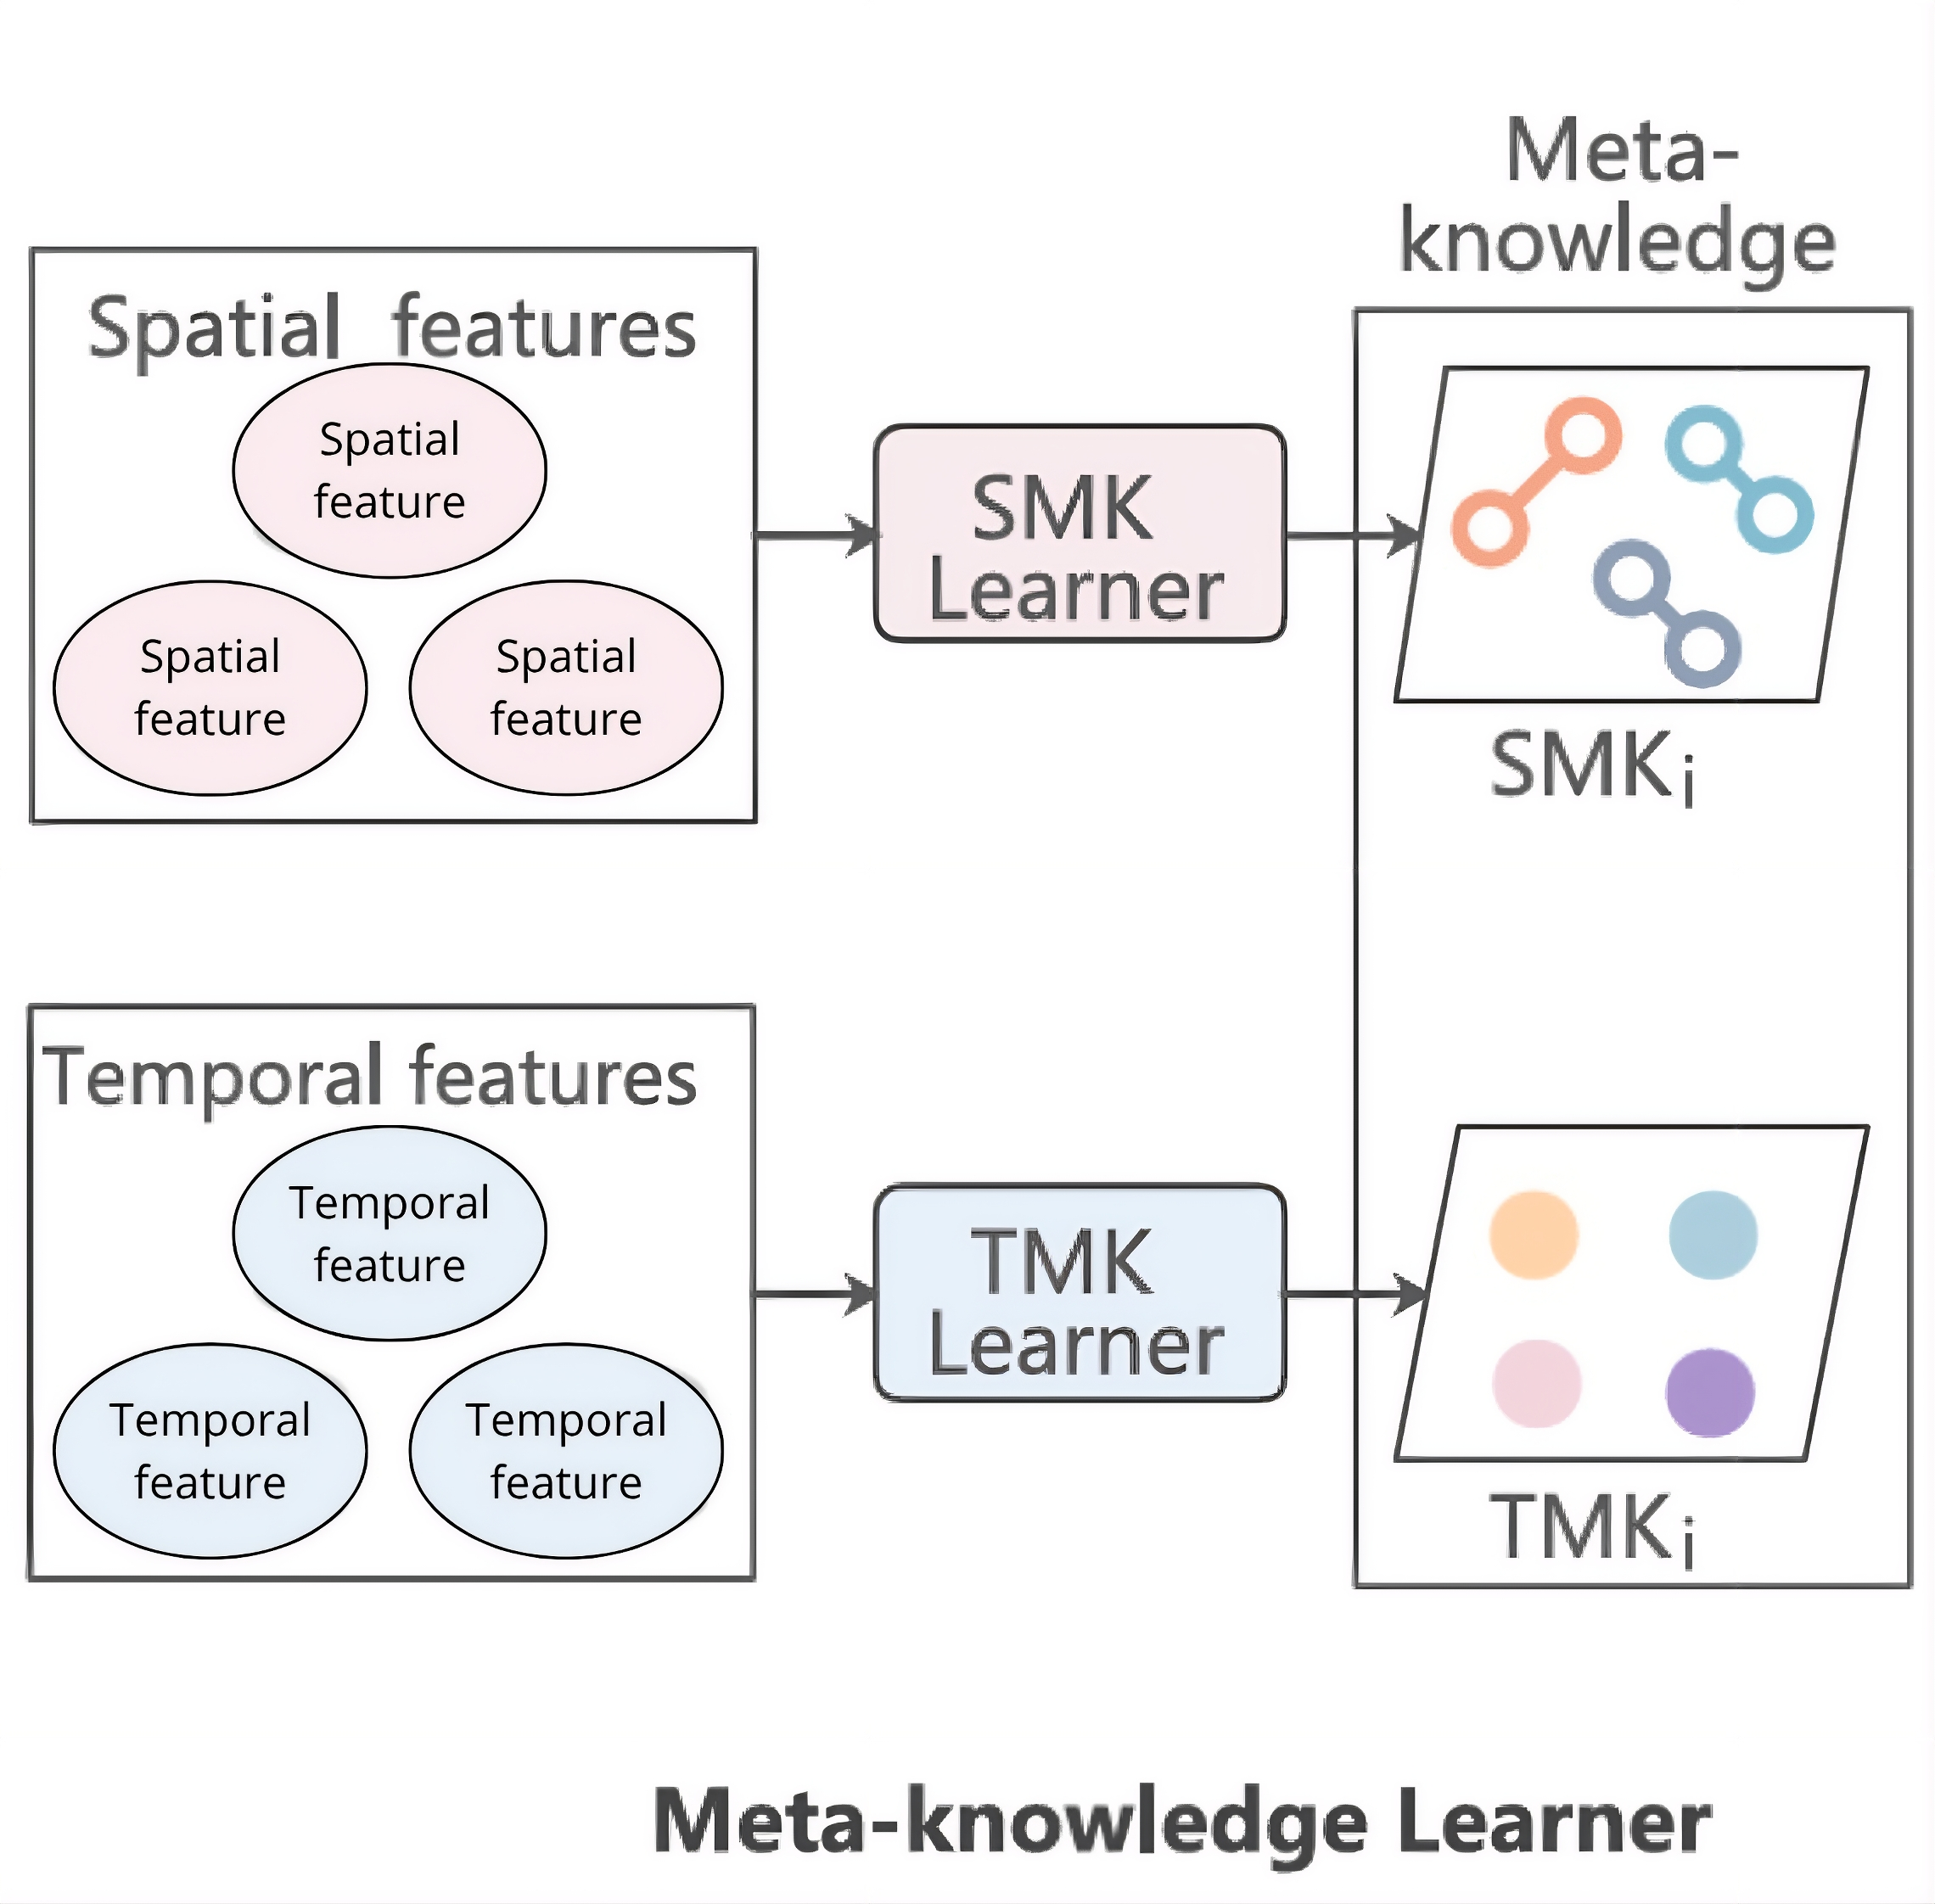
\includegraphics[width=0.7\textwidth]{meta_knowledge_learner.png}
  \caption{Il Meta-knowledge Learner: le meta-feature spaziali e temporali
    grezze vengono elaborate rispettivamente dallo SMK-Learner e dal TMK-Learner,
    producendo gli embedding $\mathrm{SMK}(i)$ e $\mathrm{TMK}(i)$ usati da
    Meta-GAT e Meta-LSTM. Adattato da \citet{wang2022metastgat}.}
  \label{fig:meta-knowledge-learner}
\end{figure}

Le meta-feature $x^{\mathrm{smk}}_i$ e $x^{\mathrm{tmk}}_i$ sono pensate per fornire al modello informazioni aggiuntive
che ne consentano una migliore specializzazione rispetto al contesto specifico di ciascun incrocio.

Il vettore spaziale $x^{\mathrm{smk}}_i \in \mathbb{R}^{26}$ concatena cinque gruppi di feature, ciascuno variabile da nodo a nodo:
\begin{itemize}
  \item pressione per corsia [12]: per ciascuna corsia, la differenza tra i veicoli in ingresso sulla corsia e la media dei veicoli sulle corsie in uscita raggiungibili da essa, divisa per 30;
  \item numero di incroci adiacenti [1]: frazione tra il numero di vicini del nodo e il massimo previsto dalla topologia a griglia (4), distingue quindi un incrocio d'angolo, di bordo o interno;
  \item differenza tra la pressione media propria e quella di ciascun incrocio adiacente [4]: per ciascuno dei vicini, la pressione media delle 12 corsie del nodo meno quella del vicino, con zero-padding negli slot oltre il numero di vicini effettivamente presenti;
  \item asimmetria di pressione tra le corsie N/S e le corsie E/O dello stesso nodo [1]: media della pressione sulle 6 corsie N/S meno la media sulle 6 corsie E/O;
  \item pressione per fase [8]: la stessa quantità usata da MaxPressure (§\ref{sec:baseline}) per decidere la fase da selezionare, una componente per ciascuna delle 8 fasi.
\end{itemize}
Il costo di raccolta di queste feature si limita a sensori con la stessa capacità visiva già richiesta per lo stato principale e per il reward, sia sulle corsie in ingresso sia su quelle in uscita: le feature di pressione si misurano semplicemente contando i veicoli su queste corsie, mentre il numero di incroci adiacenti è un dato topologico costante per ciascun incrocio.

Il vettore di meta-feature temporali $x^{\mathrm{tmk}}_i \in \mathbb{R}^{25}$
concatena invece tre diversi tipi di informazione, tutte variabili nel tempo all'interno dello stesso nodo:
\begin{itemize}
  \item variazione della coda per corsia rispetto a 3 passi precedenti [12]: per ciascuna corsia, differenza tra il numero di veicoli in coda all'istante corrente e quello di 3 step prima;
  \item durata di permanenza della fase corrente [1]: numero di step consecutivi in cui la fase è rimasta attiva, saturato e normalizzato in $[0,1]$ rispetto a un tetto di 2 step, oltre il quale la maschera anti-starvation impone comunque un cambio di fase;
  \item deviazione standard della coda per corsia sulla finestra recente [12]: calcolata sugli ultimi 5 step disponibili.
\end{itemize}
Anche queste feature vengono calcolate a partire da informazioni disponibili nel dataset e non richiedono strumenti aggiuntivi.

Si noti come nessuna di queste feature entri anche nello stato principale: la scelta
è legata alla volontà di non appesantire lo stato del sistema, sfruttando le stesse
per agire direttamente sui pesi che regolano la trasmissione dell'informazione.

\subsection{Meta-GAT}
\label{subsec:meta-gat}

La versione meta delle GAT usate in STGAT riprende la struttura architetturale delle stesse,
ma implementa delle modifiche mirate a consentire ai layer di apprendere regole di aggregazione spaziale
dipendenti dalle caratteristiche del singolo nodo.
I valori assegnati a $Q, K, V$ rimangono invariati, sia per il modulo spaziale
($Q=K=V=e_j^t$) sia per il modulo spazio-temporale ($Q=e_j^t$, $K=V=x_i^t$).
L'unica differenza riguarda l'inserimento, nel punteggio di compatibilità dell'Equazione~\ref{eq:stgat-attn},
di una trasformazione lineare per nodo che in STGAT non esiste: il modulo CS
riceve il proprio meta-embedding da $\mathrm{SMK}(i)$, il modulo CST da
$\mathrm{TMK}(i)$, in modo che la regola di attenzione spaziale e quella
spazio-temporale si adattino a caratteristiche locali diverse.
In particolare, per ciascun nodo $i$ e ciascuna testa $h$:
\[ W_{j,h}^{(i)}, \, b_{j,h}^{(i)} = \mathrm{MLP}_{\mathrm{GAT,smk},h}^{(i)}\big( \mathrm{SMK}(i) \big) \in \mathbb{R}^{d_h \times d_h}, \mathbb{R} \]
per il modulo spaziale, e
\[ W_{k,h}^{(i)}, \, b_{k,h}^{(i)} = \mathrm{MLP}_{\mathrm{GAT,tmk},h}^{(i)}\big( \mathrm{TMK}(i) \big) \in \mathbb{R}^{d_h \times d_h}, \mathbb{R} \]
per il modulo spazio-temporale,
dove le iper-reti $\mathrm{MLP}$ sono composte da due layer.
E dunque, per ogni nodo $u \in \mathcal{N}(i)$:
\begin{equation}
  \varphi_h(i,u) = \frac{\big(W_h^{(i)} Q_h(i)\big) \cdot K_h(u) + b_h^{(i)}}{\sqrt{d_h}} ,
  \label{eq:metagat-attn}
\end{equation}
\[ \alpha_h(i,u) = \frac{\exp(\varphi_h(i,u))}{\sum_{u' \in \mathcal{N}(i)} \exp(\varphi_h(i,u'))} ,\]
\[ z_h(i) = \sum_{u \in \mathcal{N}(i)} \alpha_h(i,u)\, V_h(u) ,\]
\[ z(i) = \big[z_1(i) \,\|\, \dots \,\|\, z_H(i)\big] \in \mathbb{R}^{d_1} ,\]
con $W_h^{(i)}$ e $b_h^{(i)}$ relativo al proprio modulo di riferimento.
La Figura~\ref{fig:meta-gat-diagramma} mette a confronto i due moduli appena
descritti, evidenziando come SMK e TMK alimentino iper-reti distinte per
generare i pesi $(W,b)$ specifici di ciascuno.

\begin{figure}[htbp]
  \centering
  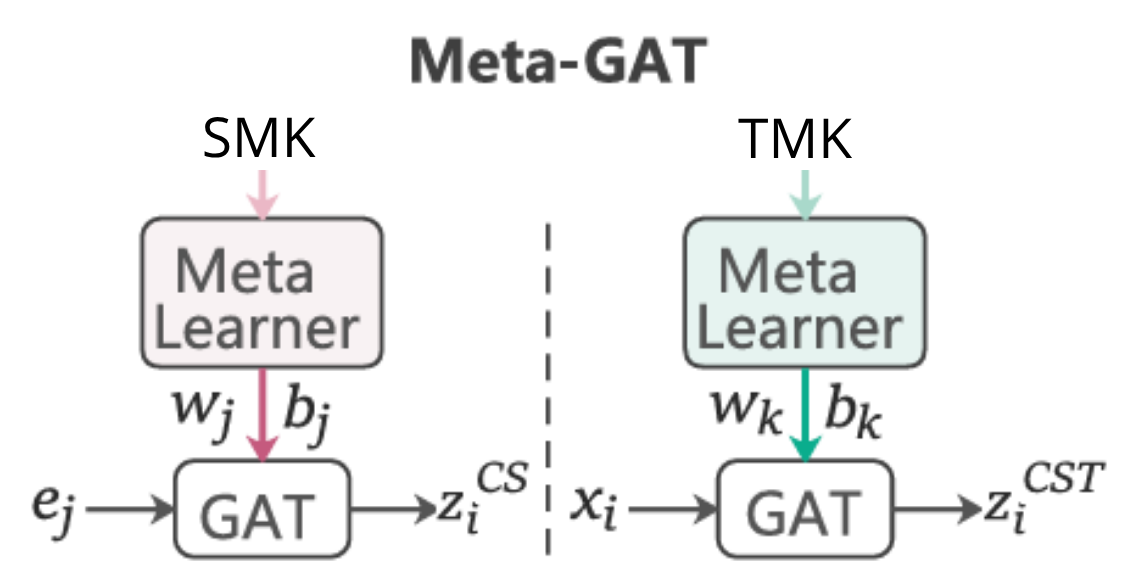
\includegraphics[width=0.8\textwidth]{meta_gat_diagramma.png}
  \caption{Meta-GAT: il modulo CS (sinistra) genera i pesi $(W_j, b_j)$ della
    propria GAT a partire da $\mathrm{SMK}$, il modulo CST (destra) genera
    $(W_k, b_k)$ a partire da $\mathrm{TMK}$; entrambi producono l'output $z_i$
    del rispettivo modulo. Adattato da \citet{wang2022metastgat}.}
  \label{fig:meta-gat-diagramma}
\end{figure}

\subsection{Meta-LSTM}
\label{subsec:meta-lstm}

Meta-LSTM applica alla cella ricorrente di STGAT
la stessa generalizzazione che Meta-GAT applica al \emph{graph attention}:
i pesi $W_{(f, \iota, o, g)}$ e i bias $b_{(f, \iota, o, g)}$ condivisi in STGAT da ogni nodo della rete,
sono qui sostituiti da pesi e bias generati individualmente per ogni nodo.

Un MLP a due layer per ciascun gate genera, dal solo $\mathrm{TMK}(i)$, i pesi \\
$W_{(f, \iota, o, g)}^{(i)} \in \mathbb{R}^{2d_1 \times d_1}$ e i bias $b_{(f, \iota, o, g)}^{(i)} \in \mathbb{R}^{d_1}$,
modificando l'Equazione~\ref{eq:stgat-lstm-gates} come segue:
\begin{equation}
  \begin{bmatrix} f_i^t \\ \iota_i^t \\ o_i^t \\ g_i^t \end{bmatrix} =
  \begin{bmatrix} \sigma \\ \sigma \\ \sigma \\ \tanh \end{bmatrix}
  \left(
  \Big(W_{\{f,\iota,o,g\}}^{(i)}\Big)^{\!\top} [\,e_i^t \,\|\, h_i^{t-1}\,] + b_{\{f,\iota,o,g\}}^{(i)}
  \right)
  \label{eq:metalstm-gates}
\end{equation}
\begin{equation}
  c_i^t = f_i^t \odot c_i^{t-1} + \iota_i^t \odot g_i^t
\end{equation}
\begin{equation}
  x_i^t = h_i^t = o_i^t \odot \tanh(c_i^t)
\end{equation}
In notazione compatta, esplicitando la sola dipendenza aggiuntiva dai pesi
generati dal meta-learner rispetto:
\begin{equation}
  \big(h_i^t,\, c_i^t\big) = \mathrm{LSTM}\Big(e_i^t \,;\, h_i^{t-1},\, c_i^{t-1} \;\Big|\; W_{\{f,\iota,o,g\}}^{(i)},\, b_{\{f,\iota,o,g\}}^{(i)}\Big), \qquad x_i^t := h_i^t.
  \label{eq:metalstm-compact}
\end{equation}
L'output $x_i^t$ alimenta il modulo CST di Meta-GAT come $K$ e $V$ (§\ref{subsec:meta-gat}),
analogamente a quanto visto con STGAT.
L'architettura appena descritta è riassunta graficamente in Figura~\ref{fig:meta-lstm-diagramma},
dove $W_{\Phi},b_{\Phi}$ indicano genericamente i pesi e i bias generati dal meta-learner.

\begin{figure}[htbp]
  \centering
  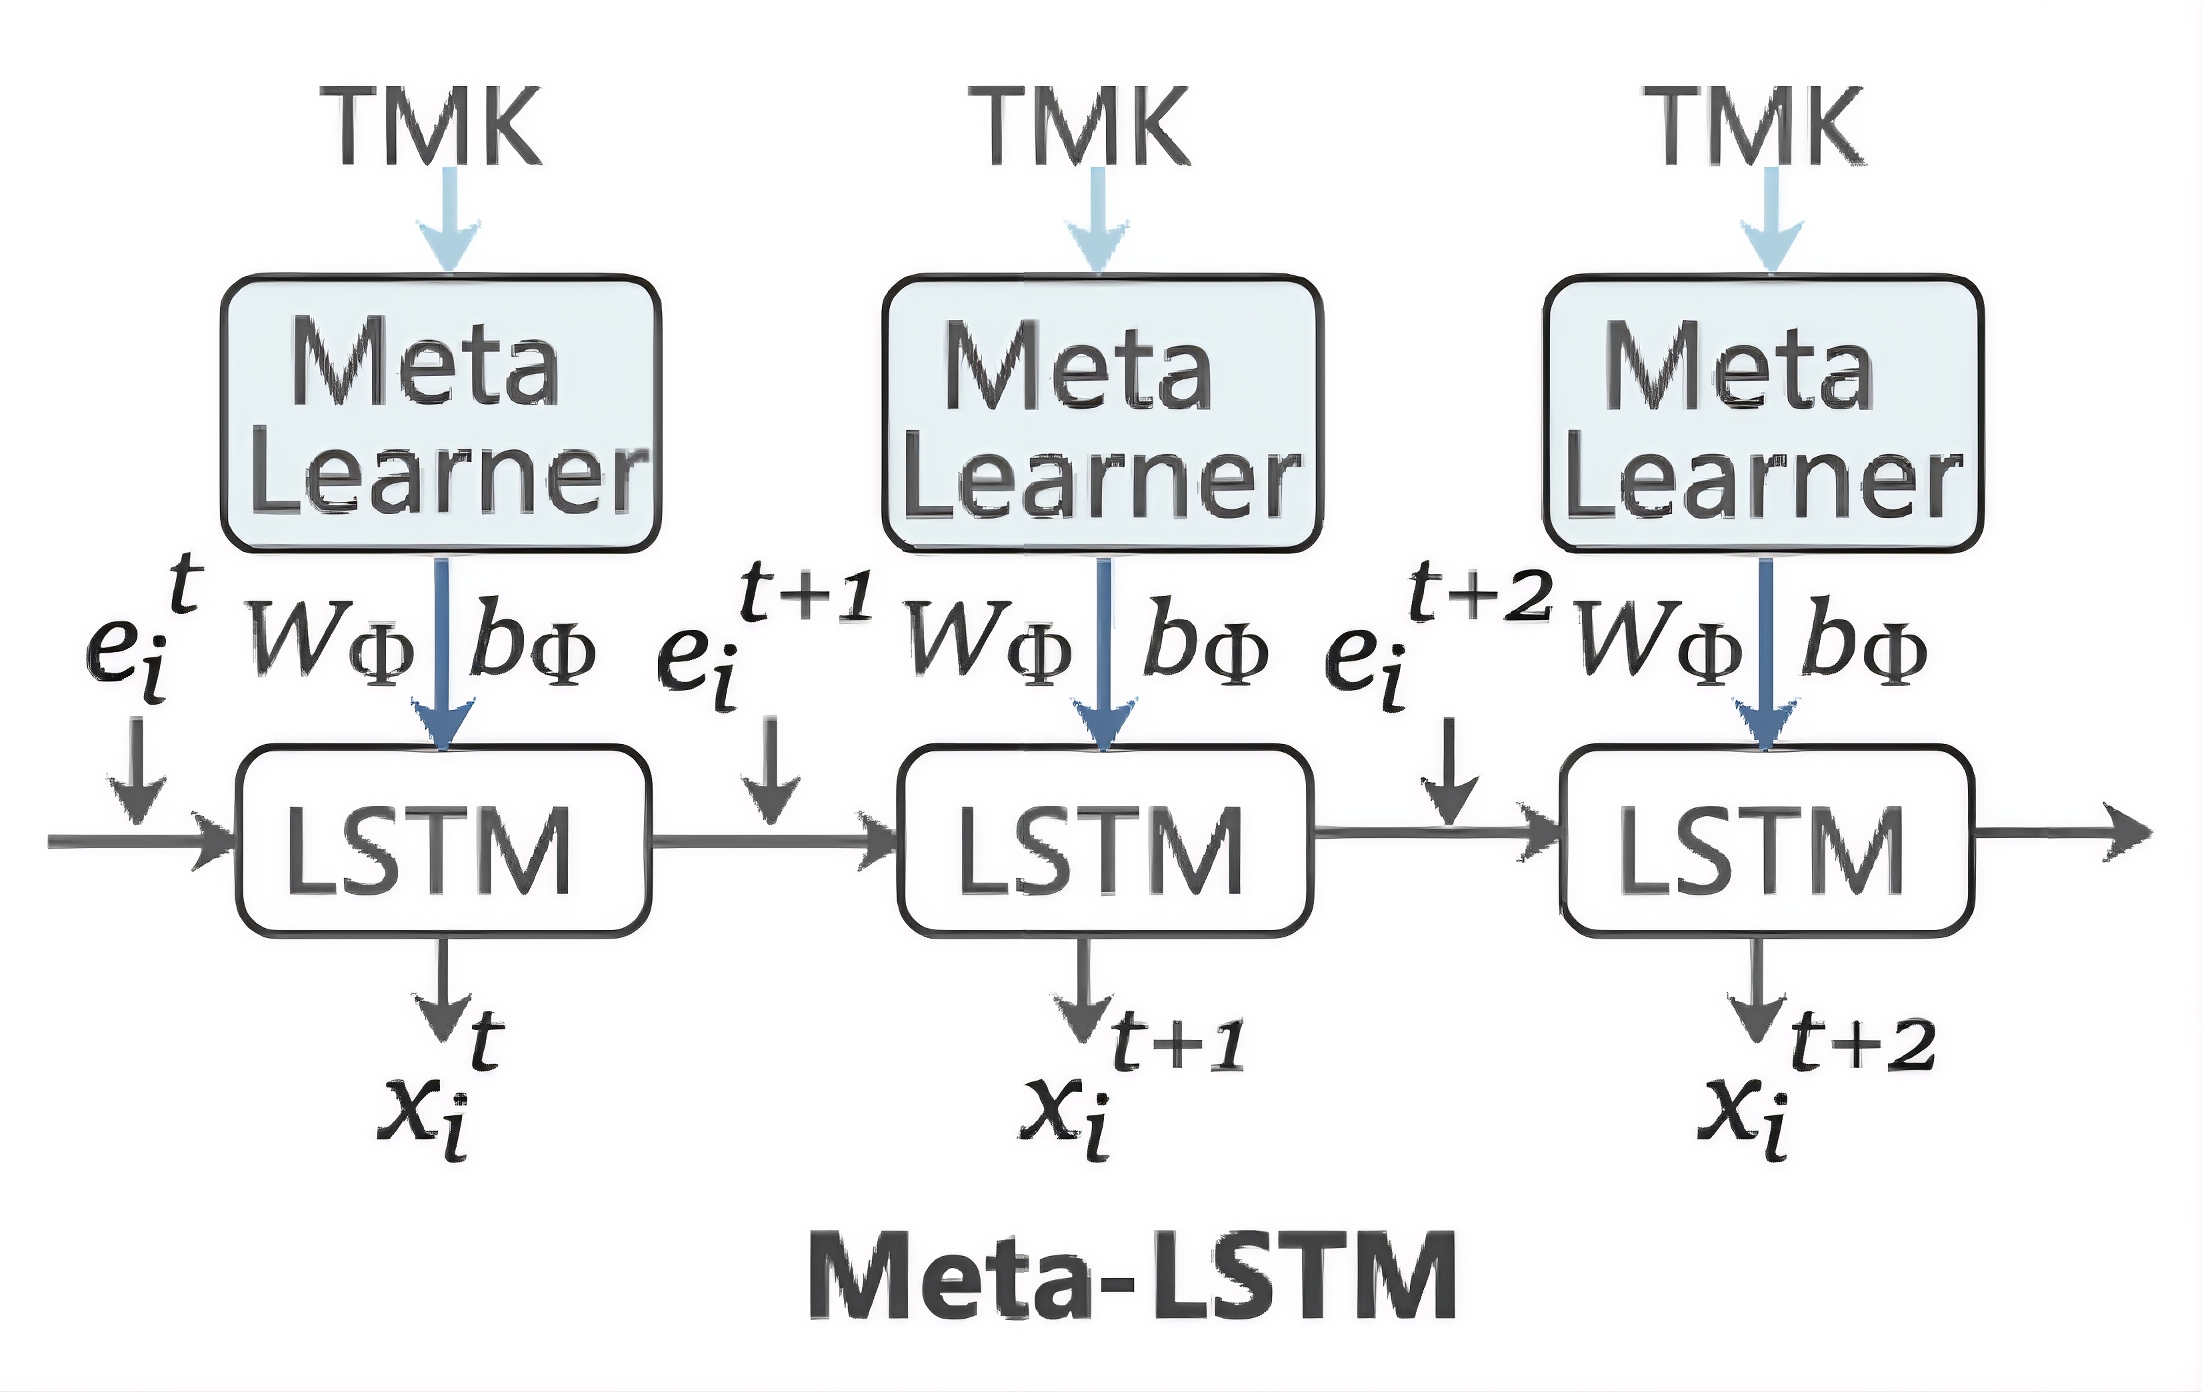
\includegraphics[width=0.85\textwidth]{meta_lstm_diagramma.png}
  \caption{Meta-LSTM "srotolata" nel tempo: a ogni istante $t$ il meta-learner
    genera, da $\mathrm{TMK}(i)$, i pesi $W_\Phi$ e $b_\Phi$ della cella LSTM
    che produce $x_i^t$ dall'input $e_i^t$ e dallo stato nascosto precedente $h_i^{t-1}, c_i^{t-1}$.
    Adattato da \citet{wang2022metastgat}.}
  \label{fig:meta-lstm-diagramma}
\end{figure}

Messi insieme, i moduli descritti in questa sezione compongono
l'architettura di Figura~\ref{fig:architettura-metastgat}, che ne riassume
il flusso complessivo dallo stato $s_i^t$ all'azione scelta.

\begin{figure}[htbp]
  \centering
  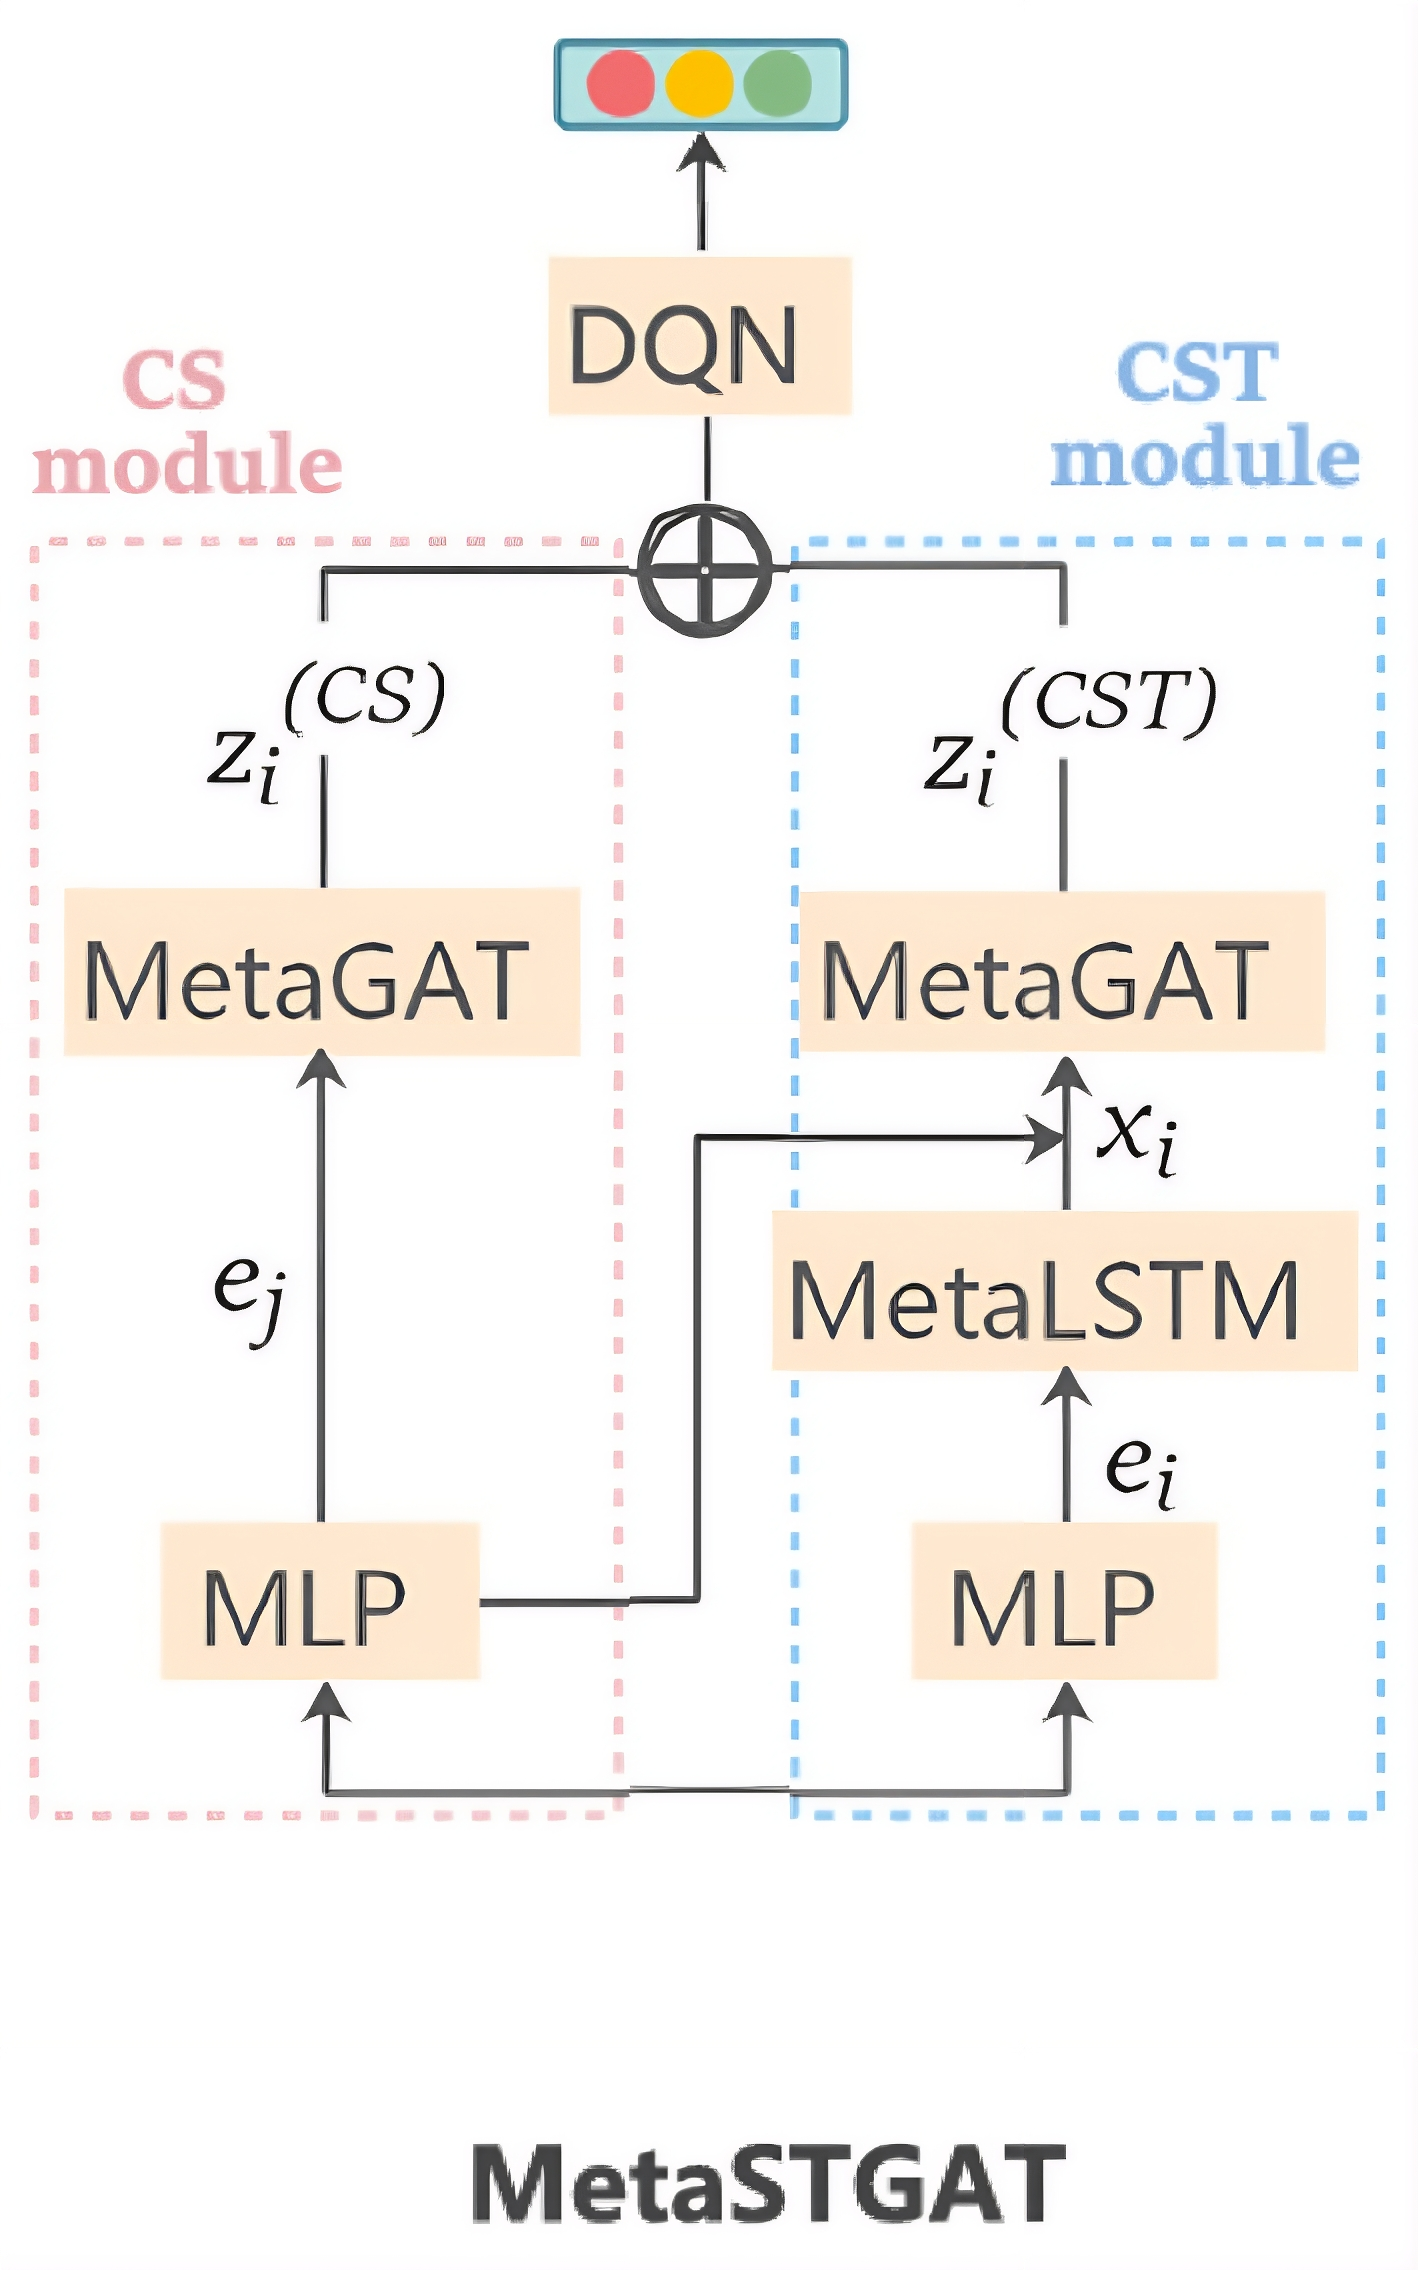
\includegraphics[width=0.5\textwidth]{architettura_metastgat.png}
  \caption{Schema a blocchi completo di MetaSTGAT: rispetto a STGAT
    (Figura~\ref{fig:stgat-architettura}), GAT e LSTM sono sostituiti dalle
    rispettive versioni meta-condizionate, con i pesi generati dagli embedding
    $\mathrm{SMK}(i)$ e $\mathrm{TMK}(i)$ del Meta-knowledge Learner. Adattato
    da \citet{wang2022metastgat}.}
  \label{fig:architettura-metastgat}
\end{figure}

\section{Differenze rispetto al modello di riferimento}
\label{subsec:framing-pro}

Il modello proposto in questo lavoro condivide con il riferimento originale \cite{wang2022metastgat}
l'intera architettura sopra descritta.
Per cercare di migliorare le prestazioni del sistema rispetto agli obiettivi di tesi,
sono state introdotte alcune modifiche, elencate di seguito e argomentate singolarmente.
L'efficacia di alcune di queste modifiche verrà analizzata più dettagliatamente nel Capitolo~\ref{cap:confronto}.

\begin{itemize}
  \item \textbf{Limitazione del campo visivo:} un contributo originale di questo studio consiste nell'introduzione di un campo visivo limitato per ciascun incrocio, per cui i dati raccolti da ogni intersezione sono circoscritti entro un raggio di visibilità $d_{\text{vis}}$.
        Le motivazioni alla base di questa implementazione sono da ricercare in due ragioni distinte: una di carattere pratico e una di carattere teorico.
        La prima mira a ridurre il gap tra simulazione e realtà, per il quale è essenziale limitare l'uso della strumentazione tecnica necessaria per la raccolta dei dati ad un'area il più circoscritta possibile.
        La seconda trova fondamento nella cinematica dei veicoli: ogni veicolo in questa simulazione raggiunge una velocità di percorrenza massima $v_{\mathrm{max}} = 11.1 \text{ m/s}$ (circa $40 \text{ km/h}$) dettata dal limite di velocità imposto su ciascuna strada.
        Ciò implica che in un intervallo di tempo fissato $\Delta t = \Delta t_{\text{green}} + \Delta t_{\text{yellow}} = 13 \text{ s}$, un veicolo possa percorrere una distanza non superiore a
        \[d_{\text{vis}} = v_{\mathrm{max}} \cdot \Delta t \approx 144.3 \text{ m} .\] Il calcolo esclude i secondi di "tutto-rosso", in cui il deflusso è interrotto.
        Il campo visivo è stato quindi ristretto anche per forzare l'agente RL a concentrarsi esclusivamente sui veicoli che una fase semaforica può effettivamente influenzare.
        Sebbene in questa architettura il cutoff spaziale sia assunto omogeneo per l'intera rete, il codice che lo implementa tiene nativamente in considerazione
        eventuali casi di limiti di velocità o intervalli temporali variabili.
        Inoltre la riduzione del campo visivo non viene applicata se la strada risulta essere più breve del cutoff stesso.
        Questa limitazione percettiva è comunque riservata ai soli modelli di reinforcement learning di questo studio e non viene applicata alla baseline (come MaxPressure).

  \item \textbf{Funzione di ricompensa:} l'articolo originale impiega esclusivamente una ricompensa di pura pressione:
        \begin{equation}
          r_i^t = -\frac{P_i^t}{100}, \qquad P_i^t = \mathrm{Incoming}_i^t - \mathrm{Outgoing}_i^t
          \label{eq:reward-paper}
        \end{equation}
        dove $P_i^t$ è la \emph{pressione dell'intersezione} $i$ al tempo $t$, ovvero la differenza tra il numero di veicoli in entrata ($\mathrm{Incoming}_i^t$) e in uscita ($\mathrm{Outgoing}_i^t$) dall'intersezione al tempo $t$.
        Il modello del presente studio sostituisce questa ricompensa con (Equazione~\ref{eq:reward-custom}):
        \[
          r_i^t = \operatorname{clip}\!\left(
          \frac{-(\mathrm{Incoming}_i^t - \mathrm{Passed}_i^t) - \alpha \cdot \mathrm{MaxRedWait}_i^t - \mathrm{Penalty}_i^t}{100},\ -2,\ 0
          \right).
        \]
        Il termine $\mathrm{Penalty}_i^t$ scatta quando la fase scelta non fa passare nessun veicolo pur essendocene in coda, il caso del "verde a vuoto": senza una penalizzazione esplicita l'agente può restare a lungo, nelle prime fasi di training, su una scelta degenere di questo tipo senza ricevere un segnale di correzione chiaro; questo valore aiuta quindi la convergenza.
        Il termine $\alpha \cdot \mathrm{MaxRedWait}_i^t$ regola invece il concetto cardine di questa tesi: l'iperparametro $\alpha$ modula quanto la ricompensa penalizzi l'attesa massima registrata a un'intersezione, permettendo di studiare il compromesso tra la riduzione del tempo di percorrenza medio e il mantenimento dell'equità tra le direzioni di marcia (Capitolo~\ref{cap:confronto}).
        Infine il \emph{clip} tra $-2$ e $0$, con il limite inferiore calibrato sperimentalmente nel corso della sperimentazione, evita che i picchi occasionali dei termini precedenti (in particolare $\mathrm{MaxRedWait}_i^t$, potenzialmente illimitato) destabilizzino l'apprendimento con aggiornamenti di gradiente sproporzionati.

  \item \textbf{Stato dell'incrocio:} il lavoro di riferimento adotta uno stato composto solo dal numero di veicoli per ciascuna corsia d'entrata $n_i^t$ e dalla fase semaforica corrente in codifica one-hot $p_i^t$ (per una dimensione totale $d_0=20$). Si aggiunge in questo studio la componente $w_i^t$, il vettore dei tempi di attesa dei veicoli da più tempo in ciascuna corsia, portando $d_0$ a 32. La motivazione è la stessa del termine di ricompensa $\mathrm{MaxRedWait}_i^t$: dare al modello un segnale diretto e locale sull'attesa, necessario perché possa correlare le proprie decisioni con l'equità tra le direzioni e non solo con il numero di veicoli in coda.

  \item \textbf{Maschera sulle azioni:} l'articolo di riferimento lascia all'agente la scelta libera tra tutte le 8 fasi a ogni passo. Si introduce qui il vincolo anti-starvation dell'Equazione~\ref{eq:action-mask} (§\ref{sec:formalizzazione}), che invalida la fase corrente se già selezionata due volte consecutive. Il numero due non è arbitrario: nelle primissime fasi di training, quando la politica è ancora vicina al caso e non ha alcuna preferenza appresa, un agente senza questo vincolo tende a bloccarsi sulla prima fase che produce un ritorno anche solo leggermente positivo, ripetendola indefinitamente; vietare la ripetizione oltre la seconda volta consecutiva rompe questo ciclo senza impedire a una fase di restare attiva per un tempo ragionevole quando è davvero la scelta migliore per due passi di fila.

  \item \textbf{Algoritmo di Deep Reinforcement Learning:} \citet{wang2022metastgat} impiega DQN standard. Il modello presentato adotta invece Double DQN \citep{vanhasselt2016double} (§\ref{sec:background-rl}), che disaccoppia selezione e valutazione dell'azione nel calcolo del target, riducendo il bias di sovrastima del valore $Q$ tipico di DQN. L'aggiornamento della target network è inoltre un \emph{soft update} (Polyak averaging, $\tau=0.01$) invece di una copia periodica integrale dei pesi: una media mobile esponenziale rende il bersaglio dell'ottimizzazione più stabile passo dopo passo, evitando i salti bruschi che una sostituzione integrale periodica introdurrebbe.

  \item \textbf{Calcolo del gradiente e aggiornamento dei pesi:} lo studio originale allena la componente ricorrente (LSTM) senza una fase di burn-in, calcolando il gradiente a partire dall'istanza campionata con lo stato ricorrente $(h,c)$ non ricostruito. Qui si campionano invece sequenze di 4 transizioni dal replay buffer, con un burn-in di 2 passi secondo lo schema R2D2 \citep{kapturowski2019r2d2}: i passi di burn-in aggiornano $(h,c)$ senza contribuire al gradiente, correggendo il disallineamento tra lo stato ricorrente osservato durante la raccolta dati e quello ricostruito in training, e poi i succesivi 2 passi servono ad aggiornare i pesi del modello. Si applica infine un \emph{gradient clipping}, limitando a norma 1 il gradiente, al fine di stabilizzare la convergenza.

  \item \textbf{Replay buffer:} il riferimento originale utilizza un replay buffer con una capacità di 10.000 transizioni e con campionamento uniforme di singole transizioni. Si adotta qui invece un replay buffer organizzato per sequenze, con Prioritized Experience Replay (PER, \citealp{schaul2016per}), la relativa correzione tramite pesi di \emph{importance sampling} (§\ref{sec:background-rl}) e una capacità di 4.800 transizioni. Il PER concentra l'aggiornamento dei pesi sulle sequenze con errore di stima più alto, anziché trattare queste ultime allo stesso modo delle transizioni già ben predette; limitare la capacità del buffer agli ultimi episodi, invece di conservarne l'intera storia, mantiene l'esperienza di training coerente con una politica che ha già imparato qualcosa, invece di continuare a ricampionare le traiettorie quasi casuali dei primissimi episodi.

  \item \textbf{Funzione di loss:} il paper di riferimento impiega l'errore quadratico medio (MSE) tra $Q$ predetto e target. Si predilige qui la Huber loss (§\ref{sec:background-rl}), più robusta agli outlier della MSE, pesata dai coefficienti di importance sampling introdotti dal PER.
\end{itemize}


\section{Meccanismi spaziali alternativi}
\label{sec:spatial-alt}

Il modulo Meta-GAT decide quanto ciascun vicino debba contribuire
all'aggiornamento di un'intersezione tramite un punteggio di compatibilità
appreso, specifico per ogni nodo (§\ref{subsec:meta-gat}).

Questa formulazione rappresenta tuttavia solo una delle possibili declinazioni del paradigma di \emph{message passing} su grafo.
Con l'obiettivo di esplorare soluzioni alternative, in questo capitolo vengono introdotte ed estese in chiave meta-learning due differenti architetture di aggregazione spaziale: Meta-GCN e Meta-SONAR.

Ogni altro componente dell'architettura (encoder di stato, meta-learner
spaziale e temporale, Meta-LSTM, testa Q-value) e la procedura di training (§\ref{sec:training}) rimarranno invariati,
cosicché ogni differenza di prestazioni che verranno misurate nel Capitolo~\ref{cap:confronto} sarà attribuibile al solo
meccanismo di aggregazione spaziale.

La prima architettura, una convoluzione grafica (GCN), rimuove il punteggio di compatibilità della GAT e lo sostituisce
con un peso fisso determinato solo dalla topologia.
Il secondo, una propagazione ondulatoria a lungo raggio chiamata SONAR \citep{trenta2025sonar},
sostituisce l'aggregazione a un passo con l'evoluzione discretizzata di un sistema dinamico su più iterazioni interne.

In entrambi i casi il principio "meta" resta identico a Meta-GAT:
i pesi dell'aggregazione sono generati da un embedding SMK/TMK per ciascun nodo, non appresi come parametro fisso condiviso.

\subsection{Meta-GCN}
\label{subsec:meta-gcn}

La GCN \citep{kipf2017gcn}, introdotta nel Capitolo~\ref{cap:background}
(Equazione~\ref{eq:gcn-aggregate}), pesa il contributo di ogni vicino con la
normalizzazione simmetrica del grado: una quantità che dipende solo dalla
topologia della rete, mai dal contenuto dello stato dei nodi coinvolti. È
dunque il termine di paragone più diretto per isolare cosa aggiunge il
punteggio di compatibilità di Meta-GAT: sostituendolo con questa regola
fissa, e lasciando invariato tutto il resto dell'architettura, ogni
differenza di prestazioni misurata nel Capitolo~\ref{cap:confronto} è
imputabile a quel solo meccanismo.

Per un nodo $i$, con $\mathcal{N}(i)$ il suo vicinato (incluso il self-loop
permanente di questo lavoro, §\ref{sec:formalizzazione}) e $\hat d_i =
  |\mathcal{N}(i)|$ il grado corrispondente, la regola originale della GCN si
scrive, per ogni vicino $u \in \mathcal{N}(i)$:
\[
  h_i' = \sigma\Big(\sum_{u \in \mathcal{N}(i)} \frac{1}{\sqrt{\hat d_i \hat d_u}}\, W\, V(u)\Big)
\]
dove $W \in \mathbb{R}^{d_1 \times d_1}$ è una matrice di pesi condivisa da
ogni nodo della rete, $\sigma$ la funzione di attivazione $\mathrm{ReLU}$ e $V(u)$ il valore
del nodo $u$ ($h_u$ nell'Equazione~\ref{eq:gcn-aggregate} del Capitolo~\ref{cap:background}).

Il principio meta genera $W$ e $b$ per ciascun nodo ricevente $i$, a partire
dal suo embedding meta $m_i$ (pari a $\mathrm{SMK}(i)$ per il modulo CS e a
$\mathrm{TMK}(i)$ per il modulo CST), tramite un'iper-rete a due strati,
in modo analogo a quanto visto in Meta-GAT:
\[
  W^{(i)}, \, b^{(i)} = \mathrm{MLP}_{\mathrm{GCN},m}^{(i)}\big(m_i\big) \in \mathbb{R}^{d_1 \times d_1}, \, \mathbb{R}
\]
Poi, per ogni nodo $i$:
\begin{equation}
  z(i) = \sigma\Bigg(\bigg(\sum_{u \in \mathcal{N}(i)} \frac{1}{\sqrt{\hat d_i \hat d_u}}\, W^{(i)}V(u)\bigg) + b^{(i)}\Bigg)
  \label{eq:metagcn}
\end{equation}
Come per Meta-GAT, il modulo CST assegna $V=x_i^t$ (l'uscita della
Meta-LSTM, §\ref{subsec:meta-lstm}) e $m_i=\mathrm{TMK}(i)$; il modulo CS
assegna $V=e_j^t$ e $m_i=\mathrm{SMK}(i)$.

\subsection{Meta-SONAR}
\label{subsec:meta-sonar}

Sia Meta-GAT sia Meta-GCN propagano informazione a un solo passo di
distanza per ogni applicazione del layer (Capitolo~\ref{cap:background}):
raggiungere un vicino a $k$ archi di distanza richiede $k$ applicazioni.
SONAR \citep{trenta2025sonar} evita questo costo modellando la propagazione
come un sistema dinamico continuo: la sua evoluzione nel tempo, non nello
spazio dei layer, porta l'informazione a più hop di distanza in un'unica
applicazione.

Il sistema si comporta come una rete di masse collegate da molle e
smorzatori, una massa per intersezione. Raccolto lo stato di tutte le $I$
intersezioni al tempo continuo $t$ in $X(t) \in \mathbb{R}^{I \times d_1}$, la sua
evoluzione è governata da un'equazione del second'ordine, un'accelerazione
e non una semplice velocità:
\begin{equation}
  \ddot X(t) = -\mathcal{L}^a X(t)\, W - D(X(t)) \odot \dot X(t) + F(X(t))
  \label{eq:sonar-wave}
\end{equation}
Tre termini, tre ruoli distinti:
\begin{itemize}
  \item $\mathcal{L}^a$ è un Laplaciano di grafo pesato da una conduttanza
        $a_{ui} \geq 0$ per arco: tira lo stato di un nodo verso quello dei suoi
        vicini, come una molla;
  \item $D(\cdot) \geq 0$ è un termine dissipativo che agisce sulla
        velocità $\dot X(t)$: frena il movimento, come un attrito;
  \item $F(\cdot)$ è una forzante esterna: inietta
        energia dall'esterno del sistema.
\end{itemize}
$W$ è, nella formulazione originale, una matrice condivisa che mescola le
$d_1$ componenti di ciascun nodo prima di applicare il Laplaciano; in questo
lavoro $W$ è l'identità, e il termine si riduce al solo accoppiamento
spaziale pesato da $a_{ui}$.

Riscritta come sistema del prim'ordine, con velocità ausiliaria $V=\dot X$,
e discretizzata con passo $h$ su $L$ iterazioni, l'aggiornamento per ogni
iterazione è:
\begin{equation}
  \begin{aligned}
    \big(\mathcal{L}^a X\big)_i & = \sum_{u \in \mathcal{N}(i)} a_{ui}\,(X_i - X_u),              \\
    V                           & \leftarrow V - h\big(\mathcal{L}^a X + D(X)\odot V - F(X)\big), \\
    X                           & \leftarrow X + h\,\tanh(V)
  \end{aligned}
  \label{eq:sonar-discrete}
\end{equation}
dove $\mathcal{N}(i)$ è il vicinato di $i$ (incluso il self-loop,
§\ref{sec:formalizzazione}) e il $\tanh$ sull'aggiornamento di $X$ è un
accorgimento di stabilità numerica, assente nella derivazione originale ma
presente nell'implementazione ufficiale di \citet{trenta2025sonar}.

La formulazione originale non ha alcuna nozione di meta-apprendimento:
$a_{ui}$, $D(\cdot)$ e $F(\cdot)$ vi sono reti a pesi fissi, condivise da
tutti i nodi. Questo lavoro applica il principio meta alla sola resistenza
$a_{ui}$, l'analogo diretto del peso appreso per coppia di nodi di Meta-GAT
e Meta-GCN: una rete a due strati genera, dall'embedding meta $m_i$ del nodo
ricevente $i$, i parametri $W_{\mathrm{res}}^{(i)} \in \mathbb{R}^{d_1
    \times 1}$ e $b_{\mathrm{res}}^{(i)} \in \mathbb{R}$, da cui
\begin{equation}
  a_{ui} = \mathrm{ReLU}\Big((X_u - X_i)W_{\mathrm{res}}^{(i)} + b_{\mathrm{res}}^{(i)}\Big)
  \label{eq:sonar-resistance}
\end{equation}
il $\mathrm{ReLU}$ garantisce $a_{ui} \geq 0$, coerente con l'interpretazione
di $a_{ui}$ come conduttanza. Dissipazione $D(\cdot)$ e forzante $F(\cdot)$
restano reti a pesi fissi applicate allo stato corrente del nodo: sono
filtri locali, non meccanismi di comunicazione tra nodi, per cui il legame
con le caratteristiche locali codificate da SMK/TMK è più debole che per la
conduttanza.

La posizione iniziale $X^0$ e la velocità iniziale $V^0$ sono prodotte in modo analogo a Meta-GAT:
per il modulo CST $X^0=x_i^t$ (l'uscita della Meta-LSTM) e $V^0=W_V\,e_j^t$ con $m_i=\mathrm{TMK}(i)$,
per il modulo CS: $X^0=e_j^t$ e $V^0=W_V\,e_j^t$ con $m_i=\mathrm{SMK}(i)$.

A differenza di Meta-GAT e Meta-GCN, dove la profondità spaziale si ottiene
impilando più applicazioni del layer a pesi indipendenti, in Meta-SONAR le
$L$ iterazioni dell'Equazione~\ref{eq:sonar-discrete} condividono gli stessi
pesi $W_{\mathrm{res}}^{(i)}$: la profondità ha quindi un costo di parametri
costante rispetto a $L$, un vantaggio strutturale dichiarato di questo
meccanismo rispetto a uno stack di layer indipendenti
\citep{trenta2025sonar}.

\section{Procedura di training e differenze dal paper originale}
\label{sec:training}

I modelli proposti, a meno di ablazioni specifiche, sono addestrati con Double DQN su sequenze campionate da un replay
buffer prioritizzato, con burn-in e Backpropagation Through Time (BPTT), Huber loss pesata dagli
\emph{importance-sampling weight} di PER, soft update della target network e
gradient clipping (§\ref{subsec:framing-pro}); l'ottimizzatore è RMSprop
per fedeltà al metodo del paper originale.

\paragraph{Funzione di loss.}
Le componenti di Double DQN, Huber loss e PER
sono definite in astratto, per una singola transizione, in
§\ref{sec:background-rl}; invece qui formalizzeremo il modo in cui si combinano sulle sequenze
ricorrenti e multi-nodo di questo lavoro.

Sia $I$ il numero di intersezioni della rete e $\ell_{\text{seq}}$ la lunghezza di una sequenza campionata $k$,
di cui le prime $\mathscr{b}$ istanze servono solo al burn-in per inizializzare lo stato ricorrente $(h,c)$,
mentre le successive $\mathscr{p} = \ell_{\text{seq}} - \mathscr{b}$ istanze contribuiscono al gradiente.
Per ciascun nodo $i$ e ciascun passo $t$ successivo al burn-in, il target Double DQN è:
\begin{equation}
  y_i^t = r_i^t + \gamma\, Q\big(s_i^{t+1},\ \operatorname*{argmax}_{a'} Q(s_i^{t+1}, a'; \theta);\ \theta^-\big)
  \label{eq:double-dqn-target}
\end{equation}
dove online e target network elaborano lo stesso stato ricorrente propagato dal burn-in.
L'errore di differenza temporale è
\[\delta_i^t = Q(s_i^t, a_i^t; \theta) - y_i^t,\]
e la loss della sequenza $k$ è la Huber loss media su tutti i nodi e i passi
validi:
\begin{equation}
  \mathcal{L}_k = \frac{1}{I\,\mathscr{p}} \sum_{i=1}^{I} \sum_{t} L_\delta(\delta_i^t)
\end{equation}
Il campionamento dal replay buffer avviene per sequenze intere, non per
transizioni isolate, di conseguenza anche la priorità del PER è definita a
livello di sequenza, come la media di $|\delta_i^t|$ sugli stessi nodi e
passi di $\mathcal{L}_k$, e aggiornata dopo ogni batch. La loss ottimizzata a
ogni passo di gradiente è la media, sulle $B$ sequenze del batch, delle loss
$\mathcal{L}_k$ pesate dai rispettivi coefficienti di importance sampling
$w_k$:
\begin{equation}
  \mathcal{L} = \frac{1}{B} \sum_{k=1}^{B} w_k\, \mathcal{L}_k .
\end{equation}
Il calcolo di \(\mathcal{L}\) è seguito da un solo passo di RMSprop,
dal gradient clipping e dal soft update della target network (§\ref{subsec:framing-pro}).

Gli iperparametri usati nel presente studio sono i seguenti:
\begin{itemize}
  \item learning rate: $10^{-3} $
  \item $\gamma$: $0.85$
  \item $d_1$: 64
  \item numero di teste $H$: 4
  \item $\varepsilon$: da 0.9 a 0.01 con decadimento esponenziale
  \item batch size $B$: 20
  \item PER buffer size $N$: 4.800 istanze
  \item lunghezza sequenze $\ell_{\text{seq}}$: 4 con burn-in 2
\end{itemize}

Ogni addestramento di questo lavoro ha una durata di 100 episodi.


\paragraph{Ciclo di training.}
Prima dell'inizio del training vero e proprio,
10 episodi di \emph{warm-up} raccolgono transizioni con $\varepsilon=1$
(azioni interamente casuali) con lo scopo di riempire il replay buffer un numero
sufficiente di istanze su cui poter addestrare l'agente.
Nel training vero e proprio, alla fine di ogni episodio, l'agente esegue 100 aggiornamenti del gradiente,
numero ereditato dal paper originale. Il valore di $\varepsilon$ decade una
volta per episodio verso il suo minimo, raggiungendolo al 60\% del numero totale
di episodi pianificati per l'addestramento.
Ricordiamo che usare $\varepsilon$-greedy come strategia di esplorazione significa che, a ogni passo di
decisione, l'agente sceglie un'azione casuale con probabilità $\varepsilon$
e altrimenti l'azione a valore $Q$ massimo secondo la stima corrente.
Oltre a questo decadimento continuo, si applica la così detta \emph{esplorazione ciclica}, per la quale un episodio ogni 10 viene eseguito
interamente a $\varepsilon=1$ anche dopo che il valore minimo di
$\varepsilon$ è stato raggiunto, senza però contribuire all'aggiornamento dei pesi in quello specifico episodio.
L'idea alla base dell'esplorazione ciclica è quella di continuare a inserire nel buffer esperienza che la politica
ormai quasi deterministica non visiterebbe più spontaneamente, al fine di
dare al modello la possibilità di non convergere su delle soluzioni sub-ottimali.
%!TEX root = ../main.tex
\chapter{Confronto}
\label{cap:confronto}

Questo capitolo descrive il protocollo sperimentale di questa tesi e ne
riporta i risultati. Definisce anzitutto le metriche di valutazione
(§\ref{sec:metriche}) e il protocollo sperimentale
(§\ref{sec:protocollo}); presenta poi il confronto di base tra le
baseline classiche e MetaSTGAT Pro insieme ai tre studi sperimentali di
questa tesi, sul peso $\alpha$ della componente di equità, sull'ablation
della procedura di addestramento e sui meccanismi di comunicazione
spaziale alternativi (§\ref{sec:confronti}), e ne riporta i risultati
(§\ref{sec:risultati-baseline}).

\section{Metriche di valutazione}
\label{sec:metriche}

Nella letteratura sul Traffic Signal Control le metriche di valutazione
proposte sono numerose.
Questo capitolo introduce le 3 metrice principali utilizzate, coerentemente con il duplice obiettivo di
questo lavoro, ovvero efficienza ed equità (come motivato nel Capitolo~\ref{cap:introduzione}):
il \emph{travel time} (tempo di viaggio) e il \emph{trip completion} (veicoli che
completano il percorso) per l'efficienza, il \emph{max wait} (l'attesa
massima registrata da un veicolo ad un incrocio) per l'equità.
C'è da sottolineare che né \emph{travel time} né
\emph{trip completion} sono metriche che appaiono esplicitamente nella
ricompensa dei modelli. Pertanto qualunque risultato su di esse sarà
l'indiretta conseguenza di come la reward ha indirizzato l'apprendimento
della policy.

\paragraph{Travel time.} Per ogni veicolo $v$, il tempo di viaggio è
\begin{equation}
  tt_v =
  \begin{cases}
    t_{\text{arrivo}}(v) - t_{\text{spawn}}(v)     & \text{se } v \text{ è arrivato entro la fine dell'episodio} \\
    t_{\text{fine episodio}} - t_{\text{spawn}}(v) & \text{altrimenti (un lower bound del vero valore)}
  \end{cases}
\end{equation}
Una delle due metriche cardini in questo studio è il travel time medio $\overline{tt}$,
ovvero la media di $ tt_v $ calcolata sull'intera popolazione di veicoli generati nell'episodio.
Tale metrica non considera soltanto i veicoli arrivati, ma include anche i
veicoli che non hanno completato il percorso entro la fine della simulazione.
La ragione è evitare un bias di sopravvivenza: un
modello che congestiona la rete e lascia arrivare solo una minoranza di
veicoli su percorsi ottimizzati otterrebbe, calcolando la media solo sui
veicoli arrivati, un risultato positivo ma non rappresentativo del comportamento reale della rete.

La seconda vera metrica cardine in questo lavoro di tesi è il travel time massimo $\overline{tt}_{\max}$,
ovvero il massimo tra tutti i travel time dei veicoli generati, anche in questo caso indipendentemente
dal completamento del percorso, per motivi analoghi a quelli descritti per il travel time medio.

\paragraph{Trip completion.} Questa metrica misura la percentuale di veicoli che hanno completato il percorso entro la
fine dell'episodio, escludendo dal totale i veicoli che in assenza di semafori e in condizioni di flusso libero non riuscirebbero comunque
a completare il proprio percorso.
In questo studio questa metrica viene indicata con $tc$. Il dettaglio di
$tc$ per ogni singolo modello e ogni singola configurazione è in
Tabella~\ref{tab:tc-adjusted}, a fine capitolo.

\paragraph{Max wait.} Questa metrica riguarda invece il massimo periodo di tempo
per cui un veicolo è rimasto bloccato allo stesso incrocio.
Dunque questo valore non si azzera nel momento in cui un veicolo avanza nella corsia, ma si annulla
soltanto se la vettura supera l'incrocio; ciò significa che max wait non considera solamente
il lasso di tempo in cui il veicolo è rimasto fermo, ma tiene conto anche del tempo in cui lo stesso si trova in movimento all'interno della corsia senza però oltrepassare l'intersezione.
Essa viene calcolata prendendo il massimo valore tra tutti i veicoli e
tutte le intersezioni.

Come per il travel time, include anche gli stalli ancora in corso al
termine dell'episodio.
In questo studio max wait viene indicato con $\text{wait}_{\max}$.

La presente metrica non va confusa con $\mathrm{MaxRedWait}_i^t$, il termine
usato nella ricompensa (Capitolo~\ref{cap:tsc-modelli}) per
penalizzare l'attesa durante il training. $\mathrm{MaxRedWait}_i^t$ è
calcolato a ogni singolo passo di decisione, su una sola intersezione alla
volta, ma soprattutto è limitata al campo visivo dell'incrocio.
$\text{wait}_{\max}$ è invece calcolato una sola volta a fine
episodio, come massimo su tutta la rete, e fa riferimento all'intera corsia.

\section{Protocollo sperimentale}
\label{sec:protocollo}

Ogni modello RL è addestrato sulle tre configurazioni di training presentate nella Tabella~\ref{tab:split}, riportata
per comodità di lettura qui sotto.

\begin{table}[htbp]
  \centering
  \footnotesize
  \begin{tabular}{@{}lllll@{}}
    \toprule
    Griglia    & Spaziatura & Profilo di traffico       & Utilizzo    & Configurazione                          \\
    \midrule
    $4\times4$ & 100m       & Complete (arteria riga 0) & Train, Test & \texttt{config\_4x4\_100m\_train1}      \\
    $4\times4$ & 100m       & Complete (arteria riga 1) & Train, Test & \texttt{config\_4x4\_100m\_train2}      \\
    $4\times4$ & 100m       & Complete (arteria riga 2) & Train, Test & \texttt{config\_4x4\_100m\_train3}      \\
    $4\times4$ & 100m       & Flat                      & Validation  & \texttt{config\_4x4\_100m\_6k\_flat}    \\
    $4\times4$ & 100m       & Peak                      & Test        & \texttt{config\_4x4\_100m\_6k\_peak}    \\
    $4\times4$ & 200m       & Flat                      & Test        & \texttt{config\_4x4\_200m\_6k\_flat}    \\
    $4\times4$ & 200m       & Peak                      & Test        & \texttt{config\_4x4\_200m\_6k\_peak}    \\
    $5\times5$ & 100m       & Flat                      & Test        & \texttt{config\_5x5\_100m\_9.4k\_flat}  \\
    $5\times5$ & 100m       & Peak                      & Test        & \texttt{config\_5x5\_100m\_9.4k\_peak}  \\
    $6\times6$ & 100m       & Flat                      & Test        & \texttt{config\_6x6\_100m\_11.5k\_flat} \\
    $6\times6$ & 100m       & Peak                      & Test        & \texttt{config\_6x6\_100m\_11.5k\_peak} \\
    \bottomrule
  \end{tabular}
\end{table}

Seguendo un ciclo fisso, le tre configurazioni si alternano episodio per
episodio. A fine training, l'ultimo checkpoint e quello che ha ottenuto il
valore di loss più basso durante l'intero addestramento sono confrontati
sulla configurazione di validazione \texttt{config\_4x4\_100m\_6k\_flat},
mediando $\overline{tt}$ su 5 seed diversi.
Questa fase serve a evitare due problemi che si concatenano tra loro.
Il primo è che in un ciclo di
apprendimento online la politica non converge necessariamente in modo
monotono, dunque gli ultimi episodi addestrati potrebbero allontanare la policy da un
punto di minimo quantomeno locale.
Il secondo è che la scelta del modello che ha registrato la loss minima non garantisce
le capacità di generalizzazione del modello, in quanto una loss bassa potrebbe
anche essere sintomo di una policy che ha soltanto memorizzato delle condizioni particolari delle
configurazioni di training, senza però aver realmente appreso una politica in grado di generalizzare.

Il modello che risulta essere migliore in questa fase di selezione, viene poi utilizzato nella fase di test.
Ogni valutazione, sia in validation sia nella batteria di test che descriveremo ora, avviene con $\varepsilon=0$:
nessuna esplorazione residua, solo la politica appresa allo stato puro. Inoltre i risultati ottenuti in ciascuna
configurazione testata, sono mediati su 5 seed diversi, analogamente a quanto fatto per $\overline{tt}$ nella fase di validazione.

Misurare la capacità di generalizzazione dei modelli è uno degli obiettivi
dichiarati di questo lavoro (Capitolo~\ref{cap:introduzione}), un asse che
gran parte della letteratura sul controllo semaforico appreso non copre
sistematicamente, in quanto la prassi più diffusa, seguita anche dall'articolo
originale di MetaSTGAT \citep{wang2022metastgat}, è addestrare e valutare un modello sulla stessa
rete stradale, senza mai trasferirlo a una topologia diversa.

Per questo motivo la batteria di test di questo lavoro include sia le 3
configurazioni di training sia 7 configurazioni aggiuntive mai viste
durante l'addestramento. Le prime permettono un confronto diretto con la
prassi di letteratura appena descritta, riportando un risultato ottenuto
nelle stesse condizioni con cui la maggior parte degli altri lavori
riporta il proprio; le seconde, assenti nella maggior parte degli studi
citati, misurano invece se le prestazioni osservate si confermano anche con il cambio
di topologia e di condizioni di traffico.

Ogni modello, RL o baseline, è dunque valutato sistematicamente sulle
stesse 10 configurazioni: le 3 varianti di training stesse (per misurare la
prestazione in-distribuzione) più 7 configurazioni mai viste in training
(4x4 a 200m invece di 100m, $5\times5$ e $6\times6$ a densità sia
\emph{flat} sia \emph{peak}), usate per misurare la generalizzazione a
topologie e densità di traffico diverse.

\section{Confronti proposti}
\label{sec:confronti}

Il confronto sperimentale di questo capitolo è organizzato in tre studi indipendenti.
Ognuno di essi isola un solo asse di variazione rispetto al
modello di riferimento ($\alpha=0.08$, MetaSTGAT a un layer) a cui ci riferiremo con il termine \emph{MetaSTGAT Pro},
lasciando invariato tutto il resto. Verranno analizzati nel seguito i tre studi proposti.
Ciascun confronto conterrà al suo interno, come riferimento, le due baseline classiche, Fixed-Time e MaxPressure, e il modello \emph{MetaSTGAT Pro}.

\subsection{Studio del peso \texorpdfstring{$\alpha$}{alpha}}

Il primo studio (§\ref{sec:risultati-baseline}) pone a confronto tre varianti del
modello MetaSTGAT Pro che differiscono solo per il valore del peso $\alpha$ riguardante la penalità anti-starvation
nella ricompensa (Eq.~\ref{eq:reward-custom}).
In particolare vengono valutati i valori di $\alpha \in \{0.08, 0.04, 0.00\}$.
È il confronto più diretto per quantificare il compromesso tra efficienza ed
equità dichiarato come obiettivo di questo lavoro.
Variando solo questo iperparametro della ricompensa, senza toccare stato o architettura,
osserveremo quanto costa in termini di travel time medio ottenere una data riduzione del travel time massimo e del max wait.

\subsection{Studio di ablazione}

Il secondo confronto (§\ref{sec:ablation-risultati}) isola sistematicamente ogni blocco di differenze
tra l'implementazione di questo lavoro e la procedura
descritta nell'articolo originale di MetaSTGAT, tramite 6 preset che
vanno dalla replica fedele del paper al modello MetaSTGAT Pro.
È un confronto necessario perché né l'uno né l'altro estremo, da soli,
spiegano il divario di prestazioni osservato tra i due: isolare un
sottosistema alla volta permette di attribuire quel divario a cause specifiche.

Ogni preset applica un gruppo coerente di scelte configurative,
isolando un sottosistema alla volta rispetto al modello MetaSTGAT Pro (§\ref{subsec:framing-pro}):

\begin{table}[htbp]
  \centering
  \small
  \begin{tabular}{@{}llp{8.5cm}@{}}
    \toprule
    Preset                   & Reward          & Cosa isola rispetto a Pro                                             \\
    \midrule
    \texttt{pro}             & \texttt{custom} & --                                                                    \\
    \texttt{temporal}        & \texttt{custom} & burn-in + BPTT sulla Meta-LSTM                                        \\
    \texttt{single\_dqn}     & \texttt{custom} & Double DQN                                                            \\
    \texttt{vanilla\_buffer} & \texttt{custom} & PER, Huber, soft update, grad clipping, warm-up, esplorazione ciclica \\
    \texttt{environment}     & \texttt{paper}  & campo visivo, feature dello stato $w_i^t$, maschera fasi consecutive  \\
    \texttt{paper}           & \texttt{paper}  & Replica fedele di Wang et al. (2022)                                  \\
    \bottomrule
  \end{tabular}
  \caption{Preset di ablazione e sottosistema isolato da ciascuno. La reward \texttt{custom} è definita da Eq. (\ref{eq:reward-custom}), mentre la reward \texttt{paper} è definita da Eq. (\ref{eq:reward-paper}).}
  \label{tab:ablation-preset}
\end{table}

\subsection{Studio sui meccanismi spaziali}

Il terzo studio (§\ref{sec:confronto-spaziale}) sostituisce il solo
meccanismo di comunicazione spaziale tra intersezioni di MetaSTGAT Pro.
Vengono testate le seguenti varianti già introdotte nel Capitolo \ref{sec:spatial-alt}:
\begin{itemize}
  \item Meta-GAT (il riferimento, a un layer come nella formulazione standard e a due layer)
  \item Meta-GCN (a uno e due layer)
  \item Meta-SONAR (a uno e due layer)
\end{itemize}

È il confronto che verifica se il beneficio osservato dipenda
specificamente dal meccanismo di attenzione appreso, o se una qualunque
forma di condivisione spaziale dell'informazione tra nodi vicini produca
risultati equivalenti.

\section{Risultati}
\label{sec:risultati-baseline}

I tre studi del precedente capitolo (§\ref{sec:confronti}) sono presentati
secondo uno schema comune: una tabella mediata sulle 3 configurazioni di
training, una corrispondente sulle 7 di test, un plot overlay che le
riassume visivamente, un plot della variazione percentuale delle metriche principali rispetto a
MaxPressure, gli eventuali casi particolari osservabili solo scendendo
alla singola configurazione, chiusi da una discussione che include, dove il risultato non
era quello atteso, una possibile spiegazione.
In queste tabelle, dallo studio sul peso $\alpha$ in poi, sono evidenziati
in grassetto i due risultati migliori di ogni colonna, Fixed-Time incluso;
nelle due tabelle del confronto di base (§\ref{sec:risultati-base}), che
hanno solo tre righe, resta invece in grassetto il solo valore migliore.

Fixed-Time, MaxPressure e MetaSTGAT Pro ($\alpha=0.08$, il modello di
riferimento di questo lavoro) compaiono in ciascuno dei tre studi.
Dunque, per non ripetere la stessa discussione su questi tre riferimenti di base,
la sottosezione seguente li confronta da soli,
mentre le sottosezioni successive approfondiranno i rispettivi confronti
(peso $\alpha$, ablazione, meccanismi spaziali).

\subsection{Fixed-Time, MaxPressure e Pro: il confronto di base}
\label{sec:risultati-base}

\begin{table}[htbp]
  \centering
  \begin{tabular}{@{}lrrrr@{}}
    \toprule
    Modello                       & $\overline{tt}$ (s) & $tt_{\max}$ (s) & wait$_{\max}$ (s) & $tc$ $(\%)$   \\
    \midrule
    Fixed-Time                    & 339.3               & 1030.0          & \textbf{470.0}    & 84.9          \\
    MaxPressure                   & \textbf{161.9}      & 1070.0          & 955.0             & \textbf{96.6} \\
    MetaSTGAT Pro ($\alpha=0.08$) & 176.7               & \textbf{675.0}  & 630.0             & 95.7          \\
    \bottomrule
  \end{tabular}
  \caption{Travel time medio, massimo, max wait e trip completion dei tre
    controllori presenti in ogni studio di questo capitolo, mediati sulle 3
    configurazioni di training.}
  \label{tab:base-train}
\end{table}

\begin{table}[htbp]
  \centering
  \begin{tabular}{@{}lrrrr@{}}
    \toprule
    Modello                       & $\overline{tt}$ (s) & $tt_{\max}$ (s) & wait$_{\max}$ (s) & $tc$ $(\%)$   \\
    \midrule
    Fixed-Time                    & 460.7               & 1496.1          & 1289.1            & 79.9          \\
    MaxPressure                   & \textbf{238.3}      & 1647.4          & 1626.0            & 88.5          \\
    MetaSTGAT Pro ($\alpha=0.08$) & 242.2               & \textbf{1049.6} & \textbf{954.0}    & \textbf{90.1} \\
    \bottomrule
  \end{tabular}
  \caption{Come Tabella~\ref{tab:base-train}, mediata sulle 7 configurazioni
    di test.}
  \label{tab:base-test}
\end{table}

Fixed-Time è il controllore peggiore su quasi ogni metrica di riferimento,
con l'unica eccezione del max wait in training (470.0s, il più basso dei tre):
la rotazione fissa delle fasi impone per costruzione un
limite alla durata di ogni attesa, un vincolo che le configurazioni di
training, meno dense, non arrivano a violare.
Questo approccio però non coordina il flusso tra le intersezioni, motivo per cui
questo risultato non si ripropone nella batteria di test dove il traffico è più intenso,
con il max wait che peggiora notevolmente.
Non osservando mai lo stato della rete, resta comunque il limite superiore di
travel time che qualunque strategia appresa dovrebbe poter migliorare.
MaxPressure e MetaSTGAT Pro lo battono nettamente sulle restanti metriche,
confermando che la regola reattiva alla base di MaxPressure coglie un segnale reale nello stato della rete.

Tra MaxPressure e MetaSTGAT Pro il confronto è più sfumato. In training e in tesing MaxPressure
resta il modello con il travel time medio più basso in assoluto (rispettivamente 161.9s e 238.3s),
coerente con la sua ottimalità di portata a livello di rete;
MetaSTGAT Pro paga per questo un travel time leggermente peggiore sia in training (176.7s, +9.1\%) sia in test (242.2s, +1.7\%).
Per quanto riguarda il max wait però il rapporto si inverte nettamente:
MetaSTGAT Pro registra un valore il 34\% più basso di MaxPressure in training e il 41\% più basso in test
(Tabelle~\ref{tab:base-train}-\ref{tab:base-test}).
Questi risultati introducono il compromesso al centro di questo lavoro, discusso nella sua forma
completa al variare di $\alpha$ nella prossima sottosezione.
Da notare è il fatto che rispetto alle prestazioni di MaxPressure, il modello MetaSTGAT Pro
ottiene risultati migliori nel training piuttosto che nel test: quanto ottenuto conferma sia
l'importanza di un controllo coordinato tra semafori quando la densità veicolare aumenta, sia
le capacità di generalizzazione acquisita dal modello MetaSTGAT Pro.

Il basso max wait di Fixed-Time in training merita un chiarimento: il suo
$tt_{\max}$ (1030.0s) resta più del doppio del suo stesso max wait
(470.0s), mentre per MaxPressure e per MetaSTGAT Pro i due valori restano
vicini (rispettivamente 1070.0s contro 955.0s, e 675.0s contro 630.0s). La
causa è strutturale: la rotazione fissa delle fasi non produce mai un
blocco estremo isolato, ma un'attesa moderata che si ripete, quasi
identica, a ogni incrocio della rete; il $tt_{\max}$ osservato è dunque la
somma di molti contributi distribuiti lungo l'intero percorso del
veicolo, non il riflesso di un singolo episodio. Negli altri due
controllori vale il caso opposto: un max wait elevato è quasi sempre un
episodio isolato su un solo incrocio, che da solo spiega quasi per intero
il $tt_{\max}$ corrispondente, con il resto del tragitto gestito in modo
efficiente.

Sul completamento ($tc$) la separazione più netta è quella tra Fixed-Time
e tutti gli altri modelli di questo capitolo: 84.9\%/79.9\%
(training/test) contro un intervallo compreso tra il 95.0\% e il 98.3\% in
training e tra l'88.9\% e il 95.8\% in test per ogni altra variante
(Tabella~\ref{tab:tc-adjusted}, a fine capitolo); l'unica
eccezione parziale è MetaSTGCN, il cui completamento più basso è discusso
a parte in §\ref{sec:confronto-spaziale}. Con questo unico scarto
rilevante già osservato qui, le sottosezioni seguenti non ripetono la
discussione di $tc$ configurazione per configurazione: si limitano a
segnalarne la tendenza generale, rimandando alla stessa tabella per il
dettaglio completo.

\subsection{Studio del peso \texorpdfstring{$\alpha$}{alpha}: risultati}
\label{sec:risultati-alpha}
\label{sec:equita-alpha}

Questa sottosezione confronta i due controllori di riferimento
(§\ref{sec:risultati-base}) con le tre varianti del modello Pro che
differiscono solo per il peso $\alpha$ della penalità anti-starvation,
con $\alpha \in \{0.08, 0.04, 0.00\}$.

\begin{table}[htbp]
  \centering
  \begin{tabular}{@{}lrrr@{}}
    \toprule
    Modello                       & $\overline{tt}$ (s) & $tt_{\max}$ (s) & wait$_{\max}$ (s) \\
    \midrule
    Fixed-Time                    & 339.3               & 1030.0          & \textbf{470.0}    \\
    MaxPressure                   & \textbf{161.9}      & 1070.0          & 955.0             \\
    MetaSTGAT Pro ($\alpha=0.08$) & 176.7               & \textbf{675.0}  & \textbf{630.0}    \\
    MetaSTGAT Pro ($\alpha=0.04$) & \textbf{170.1}      & \textbf{750.0}  & 690.0             \\
    MetaSTGAT Pro ($\alpha=0.00$) & 178.6               & 925.0           & 885.0             \\
    \bottomrule
  \end{tabular}
  \caption{Travel time medio, massimo e max wait, mediati
    sulle 3 configurazioni di training.}
  \label{tab:risultati-train}
\end{table}

\begin{table}[htbp]
  \centering
  \begin{tabular}{@{}lrrr@{}}
    \toprule
    Modello                       & $\overline{tt}$ (s) & $tt_{\max}$ (s) & wait$_{\max}$ (s) \\
    \midrule
    Fixed-Time                    & 460.7               & 1496.1          & 1289.1            \\
    MaxPressure                   & \textbf{238.3}      & 1647.4          & 1626.0            \\
    MetaSTGAT Pro ($\alpha=0.08$) & 242.2               & \textbf{1049.6} & \textbf{954.0}    \\
    MetaSTGAT Pro ($\alpha=0.04$) & \textbf{236.4}      & \textbf{1181.6} & \textbf{1125.9}   \\
    MetaSTGAT Pro ($\alpha=0.00$) & 248.7               & 1569.9          & 1539.4            \\
    \bottomrule
  \end{tabular}
  \caption{Come Tabella~\ref{tab:risultati-train}, mediata sulle 7
    configurazioni di test.}
  \label{tab:risultati-test}
\end{table}

Sul travel time medio ciò che verrebbe naturale attendersi è che
al crescese del valore di $\alpha$ la metrica in questione peggiori, con
le due configurazioni prive di penalità anti-starvation, MaxPressure e $\alpha=0.00$, che risulterebbero essere le
migliori, in quanto nessuna delle due paga un compromesso con l'equità, quindi
nessuna dovrebbe peggiorare travel time medio in cambio di un vantaggio che non
persegue.
Mentre questa analisi preliminare su $\alpha$ si conferma per i modelli con $\alpha=0.08$ e $\alpha=0.04$,
$\alpha=0.00$ risulta essere la peggiore delle tre varianti Pro su
questa metrica in entrambi i regimi (178.6s in training contro 176.7s di
$\alpha=0.08$, 248.7s in test contro 242.2s). Una causa plausibile è che
con $\alpha=0$ il termine di ricompensa legato all'attesa scompare, ma il
vettore $w_i^t$ resta nello stato osservato dalla rete
(§\ref{sec:formalizzazione}); la rete continua quindi a vedere un segnale
che la ricompensa non penalizza più causando un disallineamento tra stato e
obiettivo che può disturbare l'addestramento.

Un ulteriore risultato da sottolineare è quello ottenuto con $\alpha=0.04$ sul travel time medio in test, che non solo risulta essere il migliore tra le varianti del modello Pro,
ma supera anche MaxPressure (236.4s contro 238.3s), confermando che una quantità di penalità anti-starvation non nulla ma sufficientemente contenuta non ostacola necessariamente la performance su travel time medio.
Il risultato regge sia sulla media assoluta sia sulla media delle variazioni
percentuali per singola configurazione (Figura~\ref{fig:diffpct-alpha}),
quindi non è l'effetto di poche configurazioni favorevoli: è un segnale
che la struttura coordina bene il traffico, con un margine che cresce
proprio sulle topologie più complesse e dense.

\begin{figure}[htbp]
  \centering
  \begin{subfigure}[t]{0.48\textwidth}
    \centering
    \includegraphics[width=\linewidth]{pro_alpha_train.png}
    \caption{Configurazioni di training}
  \end{subfigure}
  \hfill
  \begin{subfigure}[t]{0.48\textwidth}
    \centering
    \includegraphics[width=\linewidth]{pro_alpha_test.png}
    \caption{Configurazioni di test}
  \end{subfigure}
  \caption{Travel time medio (fascia scura), max wait (fascia intermedia) e
    travel time massimo (fascia chiara) per lo sweep su $\alpha$, stessi dati
    delle Tabelle~\ref{tab:risultati-train}-\ref{tab:risultati-test}.}
  \label{fig:overlay-pro-alpha}
\end{figure}

\begin{figure}[htbp]
  \centering
  \begin{subfigure}[t]{0.48\textwidth}
    \centering
    \includegraphics[width=\linewidth]{diff_pct_alpha_train.png}
    \caption{Configurazioni di training}
  \end{subfigure}
  \hfill
  \begin{subfigure}[t]{0.48\textwidth}
    \centering
    \includegraphics[width=\linewidth]{diff_pct_alpha_test.png}
    \caption{Configurazioni di test}
  \end{subfigure}
  \caption{Variazione percentuale di travel time medio e massimo rispetto a
    MaxPressure (riferimento a 0\%) per lo studio su $\alpha$, calcolata per
    singola configurazione e poi mediata.}
  \label{fig:diffpct-alpha}
\end{figure}

Su max wait e $tt_{\max}$ invece il quadro è quello atteso: entrambe le
metriche peggiorano in modo pressoché monotono al diminuire di $\alpha$,
cioè al ridursi del peso dato al caso di starvation più estremo. Il
riferimento $\alpha=0.08$ ottiene sia il $tt_{\max}$ più basso in entrambi
i regimi, sia il max wait più basso, il 34\% in meno
di MaxPressure in training e il 41\% in meno in test. In test $\alpha=0.04$
resta comunque nettamente sotto Fixed-Time su entrambe le metriche (max
wait 1125.9s e $tt_{\max}$ 1181.6s, contro 1289.1s e 1496.1s);
$\alpha=0.00$ invece pareggia o peggiora leggermente i risultati di Fixed-Time
(max wait 1539.4s contro 1289.1s, $tt_{\max}$ 1569.9s contro 1496.1s).

Nonostante il vantaggio di $\alpha=0.04$ sul travel time medio, il resto
di questo lavoro adotta $\alpha=0.08$ come riferimento standard per gli
studi di ablazione e dei meccanismi spaziali
(§\ref{sec:ablation-risultati}, §\ref{sec:confronto-spaziale}). La ragione
è la priorità dichiarata tra le metriche di questo lavoro:
$\alpha=0.04$ è sistematicamente meno incisivo di
$\alpha=0.08$ su max wait e $tt_{\max}$, le due metriche di caso peggiore
che questa tesi tiene in primo piano, a fronte di un guadagno sul solo
travel time medio, la meno critica delle tre. $\alpha=0.08$ resta quindi
la scelta più coerente con l'obiettivo del lavoro, anche al costo di
qualche secondo in più di travel time medio.

\subsection{Studio di ablazione: risultati}
\label{sec:ablation-risultati}

Questa sottosezione confronta il modello Pro ($\alpha=0.08$, riferimento)
con i cinque preset di ablation presenti nella Tabella~\ref{tab:ablation-preset}:
\texttt{paper} (replica fedele del riferimento originale), \texttt{environment}
(campo di visibilità, $w_i^t$ e maschera azioni rimossi),
\texttt{temporal} (burn-in e BPTT disattivati), \texttt{single\_dqn}
(Double DQN sostituita da DQN) e \texttt{vanilla\_buffer} (PER, Huber, soft
update, gradient clipping, warm-up ed esplorazione ciclica disattivati),
tutti allo stesso $\alpha=0.08$ del riferimento.

\begin{table}[htbp]
  \centering
  \begin{tabular}{@{}lrrr@{}}
    \toprule
    Modello                          & $\overline{tt}$ (s) & $tt_{\max}$ (s) & wait$_{\max}$ (s) \\
    \midrule
    Fixed-Time                       & 339.3               & 1030.0          & \textbf{470.0}    \\
    MaxPressure                      & \textbf{161.9}      & 1070.0          & 955.0             \\
    Pro ($\alpha=0.08$, riferimento) & 176.7               & 675.0           & 630.0             \\
    \texttt{paper}                   & 187.8               & 950.0           & 915.0             \\
    \texttt{environment}             & 179.1               & 1065.0          & 1020.0            \\
    \texttt{temporal}                & 184.8               & \textbf{645.0}  & 605.0             \\
    \texttt{single\_dqn}             & 174.6               & \textbf{595.0}  & \textbf{485.0}    \\
    \texttt{vanilla\_buffer}         & \textbf{171.5}      & 695.0           & 560.0             \\
    \bottomrule
  \end{tabular}
  \caption{Travel time medio, massimo e max wait sui preset
    di ablazione, mediati sulle 3 configurazioni di training.}
  \label{tab:ablation-train}
\end{table}

\begin{table}[htbp]
  \centering
  \begin{tabular}{@{}lrrr@{}}
    \toprule
    Modello                          & $\overline{tt}$ (s) & $tt_{\max}$ (s) & wait$_{\max}$ (s) \\
    \midrule
    Fixed-Time                       & 460.7               & 1496.1          & 1289.1            \\
    MaxPressure                      & \textbf{238.3}      & 1647.4          & 1626.0            \\
    Pro ($\alpha=0.08$, riferimento) & 242.2               & 1049.6          & 954.0             \\
    \texttt{paper}                   & 271.1               & 1527.4          & 1513.3            \\
    \texttt{environment}             & 252.0               & 1595.6          & 1564.7            \\
    \texttt{temporal}                & 256.6               & 1169.1          & 1029.9            \\
    \texttt{single\_dqn}             & \textbf{240.6}      & \textbf{986.1}  & \textbf{838.7}    \\
    \texttt{vanilla\_buffer}         & 240.9               & \textbf{1048.3} & \textbf{804.0}    \\
    \bottomrule
  \end{tabular}
  \caption{Come Tabella~\ref{tab:ablation-train}, mediata sulle 7
    configurazioni di test.}
  \label{tab:ablation-test}
\end{table}

Sul travel time medio in training \texttt{vanilla\_buffer},
\texttt{single\_dqn}, il modello Pro ed \texttt{environment} restano in
una fascia stretta (171.5-179.1s). La stessa quasi coincidenza tra
\texttt{vanilla\_buffer}, \texttt{single\_dqn} e Pro si ripete
in test (240.6-242.2s), ma \texttt{environment} se ne stacca visibilmente (252.0s).
Il distacco non è uniforme sulle
sette configurazioni di test: sulle due a 200m è più del doppio rispetto
alla media delle cinque a 100m (+7.5\% contro +2.9\%, calcolato per
singola configurazione). La causa più diretta e più probabile è la disattivazione del
cutoff di visibilità propria di questo preset. Infatti, in seguito a
un addestramento comune su sole griglie a 100m, il passaggio a griglie a 200m
produce con il preset in questione degli stati di valori mai osservati prima, in quanto
\texttt{environment} osserva l'intera corsia e dunque registra un conteggio veicoli mai incontrato in training.
Gli altri preset invece limitano questo scarto numerico grazie al ridotto campo visivo,
aiutando di fatto il modello a generalizzare su reti con spaziatura maggiore rispetto a quella del training.

\begin{figure}[htbp]
  \centering
  \begin{subfigure}[t]{0.48\textwidth}
    \centering
    \includegraphics[width=\linewidth]{ablation_train.png}
    \caption{Configurazioni di training}
  \end{subfigure}
  \hfill
  \begin{subfigure}[t]{0.48\textwidth}
    \centering
    \includegraphics[width=\linewidth]{ablation_test.png}
    \caption{Configurazioni di test}
  \end{subfigure}
  \caption{Travel time medio, max wait e travel time massimo sui preset di
    ablation, stessi dati delle
    Tabelle~\ref{tab:ablation-train}-\ref{tab:ablation-test}.}
  \label{fig:overlay-ablation}
\end{figure}

\begin{figure}[htbp]
  \centering
  \begin{subfigure}[t]{0.48\textwidth}
    \centering
    \includegraphics[width=\linewidth]{diff_pct_ablation_train.png}
    \caption{Configurazioni di training}
  \end{subfigure}
  \hfill
  \begin{subfigure}[t]{0.48\textwidth}
    \centering
    \includegraphics[width=\linewidth]{diff_pct_ablation_test.png}
    \caption{Configurazioni di test}
  \end{subfigure}
  \caption{Variazione percentuale di travel time medio e massimo rispetto a
    MaxPressure (riferimento a 0\%) sui preset di ablation, calcolata per
    singola configurazione/seed e poi mediata.}
  \label{fig:diffpct-ablation}
\end{figure}

Su $tt_{\max}$ e $wait_{max}$, \texttt{paper} ed \texttt{environment} restano
nettamente indietro in entrambi i regimi, coerentemente con l'unico
elemento che condividono e che differisce da ogni altro preset: l'assenza del
termine legato all'attesa nella ricompensa.

Sempre sulle stesse due metriche in questione invece, i tre preset che lasciano intatti stato, ricompensa e maschera
(\texttt{temporal}, \texttt{single\_dqn}, \texttt{vanilla\_buffer}),
registrano in training i migliori risultati in assoluto tra tutti i preset considerati, modello Pro incluso.

Tuttavia, per quanto riguarda i risultati in regime di test
il quadro si inverte per \texttt{temporal}, con Pro che registra $tt_{\max}$ e $wait_{max}$ migliori.
Un'analisi sulle singole configurazioni rivela che il crollo è sistematico
e cresce con la scala della griglia: il suo $tt_{\max}$ medio per
configurazione resta vicino al riferimento sulle tre configurazioni 4x4
(855-975s) ma sale a 1218-1524s su 5x5 e 6x6.
La causa probabilmente da ricercare nel fatto che \texttt{temporal} disattiva BPTT e burn-in: senza propagazione del gradiente
lungo la sequenza né un periodo di adattamento dello stato ricorrente
all'inizio di ogni episodio, il modulo temporale della Meta-LSTM ha meno
modo di generalizzare il proprio stato interno a topologie di scala
diversa da quella di training, mentre lo stesso stato interno resta
adeguato sulla scala 4x4 già vista. La curva di training offre un
indizio indipendente coerente con questa lettura: la loss di
\texttt{temporal} resta stabilmente più alta di quella del riferimento
per l'intero addestramento, un divario compatibile con
un limite strutturale imposto dall'assenza di BPTT e burn-in.

Il vantaggio di \texttt{single\_dqn} e \texttt{vanilla\_buffer} su
$tt_{\max}$ e max wait regge anche scendendo alla singola configurazione,
senza che questo lavoro riesca a indicarne con certezza la causa. Resta
aperta una domanda distinta, che uno studio dedicato dovrebbe verificare:
se la generalizzazione di questi due preset regga altrettanto bene su
spaziature stradali diverse da quella di training. Un indizio non
conclusivo in questo senso viene dal max wait: il vantaggio di entrambi i
preset sul modello Pro, ampio sulle configurazioni 5x5 e 6x6
mai viste in training, si riduce fino a scendere al di sotto del modello Pro sulle due configurazioni
a 200m. Non possiamo pertanto dire con certezza che questi preset funzionino altrettanto bene su spaziature stradali diverse da quella di training.

\subsection{Studio sui meccanismi spaziali: risultati}
\label{sec:confronto-spaziale}

Questa sottosezione confronta il modello Pro (MetaSTGAT, un layer)
con le sue varianti a meccanismo spaziale alternativo definite in
§\ref{sec:spatial-alt}: MetaSTGAT a due layer, MetaSTGCN a uno e due
layer, e MetaSTSONAR con $L=2$ e $L=4$ ricorrenze. Tutti i modelli
condividono l'architettura residua, gli iperparametri e procedura di training.


\begin{table}[htbp]
  \centering
  \begin{tabular}{@{}lrrr@{}}
    \toprule
    Modello                          & $\overline{tt}$ (s) & $tt_{\max}$ (s) & wait$_{\max}$ (s) \\
    \midrule
    Fixed-Time                       & 339.3               & 1030.0          & \textbf{470.0}    \\
    MaxPressure                      & \textbf{161.9}      & 1070.0          & 955.0             \\
    MetaSTGAT, 1L (Pro, riferimento) & 176.7               & 675.0           & 630.0             \\
    MetaSTGAT, 2L                    & 174.6               & \textbf{635.0}  & \textbf{510.0}    \\
    MetaSTGCN, 1L                    & 248.5               & 1340.0          & 1280.0            \\
    MetaSTGCN, 2L                    & 217.8               & 1180.0          & 1160.0            \\
    MetaSTSONAR, $L{=}2$             & 170.6               & \textbf{630.0}  & 535.0             \\
    MetaSTSONAR, $L{=}4$             & \textbf{170.2}      & 660.0           & 525.0             \\
    \bottomrule
  \end{tabular}
  \caption{Travel time medio, massimo e max wait sui
    meccanismi spaziali, mediati sulle 3 configurazioni di training.}
  \label{tab:architetture-train}
\end{table}

\begin{table}[htbp]
  \centering
  \begin{tabular}{@{}lrrr@{}}
    \toprule
    Modello                          & $\overline{tt}$ (s) & $tt_{\max}$ (s) & wait$_{\max}$ (s) \\
    \midrule
    Fixed-Time                       & 460.7               & 1496.1          & 1289.1            \\
    MaxPressure                      & 238.3               & 1647.4          & 1626.0            \\
    MetaSTGAT, 1L (Pro, riferimento) & 242.2               & \textbf{1049.6} & \textbf{954.0}    \\
    MetaSTGAT, 2L                    & 246.6               & 1128.0          & 990.0             \\
    MetaSTGCN, 1L                    & 333.8               & 1659.0          & 1631.6            \\
    MetaSTGCN, 2L                    & 288.5               & 1457.6          & 1428.9            \\
    MetaSTSONAR, $L{=}2$             & \textbf{237.9}      & \textbf{1038.4} & \textbf{862.3}    \\
    MetaSTSONAR, $L{=}4$             & \textbf{238.3}      & 1119.9          & 1047.4            \\
    \bottomrule
  \end{tabular}
  \caption{Come Tabella~\ref{tab:architetture-train}, mediata sulle 7
    configurazioni di test.}
  \label{tab:architetture-test}
\end{table}

Il divario più netto di questo confronto separa MetaSTGCN dagli altri due
meccanismi. In test, entrambe le varianti
MetaSTGCN registrano valori nettamente peggiori su ogni colonna (travel time medio
288.5-333.8s contro 237.9-246.6s di MetaSTGAT/MetaSTSONAR), con un
$tt_{\max}$ e un $wait_{\max}$ che restano vicini a quelli di MaxPressure pur
trattandosi di un modello addestrato con lo stesso obiettivo di equità del
riferimento. La differenza concettuale descritta in §\ref{subsec:meta-gcn},
un peso di aggregazione fissato dalla sola topologia contro un punteggio di
compatibilità appreso per coppia di nodi, si traduce quindi in un divario di
prestazioni ampio su questo compito.
Un secondo layer in MetaSTGCN
migliora la variante a singolo layer su tutte le metriche riportate in
entrambi i regimi ($\overline{tt}$ di training 248.5$\to$217.8s,
$tt_{\max}$ di test 1659.0$\to$1457.6s, max wait di test
1631.6$\to$1428.9s): la profondità aggiuntiva compensa qui, almeno in
parte, l'assenza di un meccanismo di compatibilità appreso, pur restando
lontana dalle prestazioni di MetaSTGAT e MetaSTSONAR.

MetaSTGAT e MetaSTSONAR hanno prestazioni pressochè pari tra loro su travel
time medio e massimo; sul max wait, però, è MetaSTSONAR con $L=2$ a ottenere il
risultato migliore dell'intero confronto (862.3s in test), davanti
sia al modello Pro di riferimento (954.0s) sia alla sua variante a
due layer (990.0s).

Tra le due profondità di MetaSTSONAR, $L=2$ supera $L=4$ anche
sul $tt_{\max}$ in entrambi i regimi (630.0s contro 660.0s in training,
1038.4s contro 1119.9s in test), senza il vantaggio teorico di campo
recettivo più ampio atteso da una profondità doppia.

Aggiungere un secondo layer a MetaSTGAT, a differenza di MetaSTGCN, non produce qui un
miglioramento netto: la variante a due layer resta vicina al riferimento
su travel time medio e massimo ma peggiora leggermente il max wait in
test (990.0s contro 954.0s).

Un caso particolare nelle configurazioni di
training (Tabella~\ref{tab:wait-full}): MetaSTGCN a un layer ottiene un
max wait medio di 1280s, peggiore di MaxPressure stesso (955s), pur
condividendo con il riferimento la stessa ricompensa orientata
all'equità. È il solo modello di tutto questo lavoro, tra quelli
addestrati con il termine anti-starvation pieno, a non riuscire a battere
la baseline reattiva su questa metrica nel proprio stesso regime di
addestramento, coerentemente con la spiegazione architetturale data sopra: un
peso di aggregazione fissato dalla topologia non ha modo di imparare a
dare priorità al segnale del vicino più in sofferenza, per quanto la
ricompensa lo incentivi a farlo.

\begin{figure}[htbp]
  \centering
  \begin{subfigure}[t]{0.48\textwidth}
    \centering
    \includegraphics[width=\linewidth]{architectures_train.png}
    \caption{Configurazioni di training}
  \end{subfigure}
  \hfill
  \begin{subfigure}[t]{0.48\textwidth}
    \centering
    \includegraphics[width=\linewidth]{architectures_test.png}
    \caption{Configurazioni di test}
  \end{subfigure}
  \caption{Travel time medio, max wait e travel time massimo sui meccanismi
    spaziali, stessi dati delle
    Tabelle~\ref{tab:architetture-train}-\ref{tab:architetture-test}.}
  \label{fig:overlay-architetture}
\end{figure}

\begin{figure}[htbp]
  \centering
  \begin{subfigure}[t]{0.48\textwidth}
    \centering
    \includegraphics[width=\linewidth]{diff_pct_architetture_train.png}
    \caption{Configurazioni di training}
  \end{subfigure}
  \hfill
  \begin{subfigure}[t]{0.48\textwidth}
    \centering
    \includegraphics[width=\linewidth]{diff_pct_architetture_test.png}
    \caption{Configurazioni di test}
  \end{subfigure}
  \caption{Variazione percentuale di travel time medio e massimo rispetto a
    MaxPressure (riferimento a 0\%) sui meccanismi spaziali, calcolata per
    singola configurazione/seed e poi mediata.}
  \label{fig:diffpct-architetture}
\end{figure}

\subsection{Tabelle dei risultati.}
Sono qui di seguito riportati i risultati completi di tutti i modelli rispetto ciascuna configurazioni testata.

\begin{sidewaystable}
  \centering
  \tiny
  \begin{tabular}{@{}lrrrrrrrrrr@{}}
    \toprule
    Modello                   & Train 1 & Train 2 & Train 3 & 4x4 Pk & 4x4-200 F & 4x4-200 Pk & 5x5 F & 5x5 Pk & 6x6 F & 6x6 Pk \\
    \midrule
    Fixed-Time                & 84.6    & 85.5    & 87.9    & 84.7   & 84.0      & 81.9       & 84.4  & 82.6   & 81.5  & 80.4   \\
    MaxPressure               & 98.0    & 98.3    & 97.1    & 92.8   & 93.5      & 92.0       & 92.0  & 91.2   & 90.7  & 89.2   \\
    Pro ($\alpha$=0.08)       & 96.4    & 97.5    & 96.8    & 93.3   & 95.3      & 92.8       & 93.5  & 93.1   & 92.9  & 92.8   \\
    Pro ($\alpha$=0.04)       & 97.2    & 97.4    & 97.2    & 94.0   & 95.8      & 93.6       & 93.3  & 92.5   & 92.4  & 92.0   \\
    Pro ($\alpha$=0.00)       & 96.2    & 96.9    & 96.8    & 92.9   & 93.7      & 92.2       & 93.2  & 92.3   & 92.2  & 91.1   \\
    MetaSTGAT 2L              & 96.5    & 97.4    & 97.8    & 93.7   & 94.5      & 92.6       & 93.7  & 92.2   & 93.1  & 92.3   \\
    Ablation: paper           & 95.0    & 96.5    & 96.3    & 91.6   & 93.5      & 90.2       & 91.4  & 90.8   & 90.7  & 88.9   \\
    Ablation: temporal        & 95.8    & 95.6    & 97.0    & 92.7   & 93.4      & 91.6       & 93.2  & 92.5   & 92.8  & 92.6   \\
    Ablation: single\_dqn     & 96.8    & 97.6    & 97.0    & 93.6   & 95.6      & 93.4       & 93.3  & 92.3   & 92.5  & 92.2   \\
    Ablation: environment     & 95.9    & 96.6    & 95.7    & 91.1   & 92.8      & 90.8       & 92.1  & 91.7   & 91.4  & 89.2   \\
    Ablation: vanilla\_buffer & 96.1    & 97.7    & 97.5    & 93.8   & 95.7      & 92.9       & 93.7  & 92.8   & 92.9  & 92.0   \\
    MetaSTGCN 1L              & 90.6    & 91.1    & 91.7    & 87.2   & 88.3      & 86.2       & 88.9  & 85.8   & 86.7  & 85.1   \\
    MetaSTGCN 2L              & 93.3    & 94.8    & 93.6    & 91.0   & 92.6      & 89.8       & 91.4  & 90.2   & 90.6  & 89.4   \\
    MetaSTSONAR L=2           & 97.3    & 97.7    & 97.5    & 93.4   & 95.5      & 93.1       & 93.9  & 92.6   & 93.3  & 92.0   \\
    MetaSTSONAR L=4           & 97.2    & 97.6    & 97.6    & 93.4   & 95.1      & 92.6       & 93.2  & 92.9   & 93.3  & 92.9   \\
    \bottomrule
  \end{tabular}
  \caption{Percentuale di trip completion $tc$ per ogni modello
    e ogni configurazione, corretta escludendo dal
    denominatore i veicoli strutturalmente impossibilitati ad arrivare in
    tempo. Nessun modello scende sotto l'80\%; a parte Fixed-Time (baseline non
    adattiva) l'unico caso ricorrente sotto il 90\% è MetaSTGCN 1L.}
  \label{tab:tc-adjusted}
\end{sidewaystable}

\begin{sidewaystable}
  \centering
  \tiny
  \begin{tabular}{@{}lrrrrrrrrrr@{}}
    \toprule
    Modello                   & Train 1 & Train 2 & Train 3 & 4x4 Pk                                     & 4x4-200 F                                  & 4x4-200 Pk                                 & 5x5 F                                       & 5x5 Pk                                     & 6x6 F                                      & 6x6 Pk                                     \\
    \midrule
    Fixed-Time                & 351.6   & 342.9   & 323.3   & 437.3 {\fontsize{4}{4}\selectfont$\pm$6.4} & 415.5 {\fontsize{4}{4}\selectfont$\pm$6.7} & 438.8 {\fontsize{4}{4}\selectfont$\pm$4.9} & 459.7 {\fontsize{4}{4}\selectfont$\pm$4.7}  & 485.0 {\fontsize{4}{4}\selectfont$\pm$5.1} & 484.8 {\fontsize{4}{4}\selectfont$\pm$6.2} & 503.7 {\fontsize{4}{4}\selectfont$\pm$4.6} \\
    MaxPressure               & 165.4   & 160.2   & 160.0   & 218.8 {\fontsize{4}{4}\selectfont$\pm$2.3} & 197.3 {\fontsize{4}{4}\selectfont$\pm$4.2} & 247.8 {\fontsize{4}{4}\selectfont$\pm$2.6} & 217.8 {\fontsize{4}{4}\selectfont$\pm$3.3}  & 258.6 {\fontsize{4}{4}\selectfont$\pm$4.9} & 244.7 {\fontsize{4}{4}\selectfont$\pm$5.5} & 283.3 {\fontsize{4}{4}\selectfont$\pm$1.4} \\
    Pro ($\alpha$=0.08)       & 180.2   & 176.3   & 173.5   & 230.9 {\fontsize{4}{4}\selectfont$\pm$2.6} & 199.5 {\fontsize{4}{4}\selectfont$\pm$2.4} & 252.0 {\fontsize{4}{4}\selectfont$\pm$3.3} & 224.8 {\fontsize{4}{4}\selectfont$\pm$3.1}  & 266.7 {\fontsize{4}{4}\selectfont$\pm$3.4} & 243.3 {\fontsize{4}{4}\selectfont$\pm$3.4} & 278.6 {\fontsize{4}{4}\selectfont$\pm$4.0} \\
    Pro ($\alpha$=0.04)       & 172.5   & 169.4   & 168.4   & 223.3 {\fontsize{4}{4}\selectfont$\pm$3.1} & 196.9 {\fontsize{4}{4}\selectfont$\pm$3.4} & 248.2 {\fontsize{4}{4}\selectfont$\pm$3.8} & 213.4 {\fontsize{4}{4}\selectfont$\pm$4.6}  & 258.2 {\fontsize{4}{4}\selectfont$\pm$3.0} & 237.1 {\fontsize{4}{4}\selectfont$\pm$5.0} & 277.5 {\fontsize{4}{4}\selectfont$\pm$4.5} \\
    Pro ($\alpha$=0.00)       & 183.5   & 180.8   & 171.5   & 237.5 {\fontsize{4}{4}\selectfont$\pm$3.8} & 206.1 {\fontsize{4}{4}\selectfont$\pm$3.5} & 257.8 {\fontsize{4}{4}\selectfont$\pm$2.6} & 230.9 {\fontsize{4}{4}\selectfont$\pm$4.5}  & 269.8 {\fontsize{4}{4}\selectfont$\pm$3.7} & 247.9 {\fontsize{4}{4}\selectfont$\pm$4.6} & 290.7 {\fontsize{4}{4}\selectfont$\pm$6.0} \\
    MetaSTGAT 2L              & 181.3   & 175.0   & 167.6   & 231.8 {\fontsize{4}{4}\selectfont$\pm$3.5} & 203.7 {\fontsize{4}{4}\selectfont$\pm$2.1} & 252.7 {\fontsize{4}{4}\selectfont$\pm$2.9} & 228.8 {\fontsize{4}{4}\selectfont$\pm$3.7}  & 275.4 {\fontsize{4}{4}\selectfont$\pm$5.5} & 245.3 {\fontsize{4}{4}\selectfont$\pm$4.0} & 289.5 {\fontsize{4}{4}\selectfont$\pm$3.7} \\
    Ablation: paper           & 194.1   & 182.9   & 186.5   & 253.9 {\fontsize{4}{4}\selectfont$\pm$4.6} & 217.7 {\fontsize{4}{4}\selectfont$\pm$3.6} & 287.3 {\fontsize{4}{4}\selectfont$\pm$4.8} & 245.3 {\fontsize{4}{4}\selectfont$\pm$11.4} & 294.5 {\fontsize{4}{4}\selectfont$\pm$5.2} & 275.8 {\fontsize{4}{4}\selectfont$\pm$2.6} & 318.6 {\fontsize{4}{4}\selectfont$\pm$3.5} \\
    Ablation: temporal        & 189.8   & 190.0   & 174.6   & 247.4 {\fontsize{4}{4}\selectfont$\pm$6.4} & 213.6 {\fontsize{4}{4}\selectfont$\pm$7.0} & 262.5 {\fontsize{4}{4}\selectfont$\pm$6.8} & 240.3 {\fontsize{4}{4}\selectfont$\pm$6.0}  & 282.1 {\fontsize{4}{4}\selectfont$\pm$4.7} & 256.6 {\fontsize{4}{4}\selectfont$\pm$3.6} & 293.8 {\fontsize{4}{4}\selectfont$\pm$4.1} \\
    Ablation: single\_dqn     & 178.4   & 173.4   & 172.1   & 227.3 {\fontsize{4}{4}\selectfont$\pm$1.8} & 198.8 {\fontsize{4}{4}\selectfont$\pm$3.0} & 249.2 {\fontsize{4}{4}\selectfont$\pm$3.8} & 221.8 {\fontsize{4}{4}\selectfont$\pm$2.2}  & 266.7 {\fontsize{4}{4}\selectfont$\pm$5.0} & 241.1 {\fontsize{4}{4}\selectfont$\pm$4.3} & 279.0 {\fontsize{4}{4}\selectfont$\pm$3.5} \\
    Ablation: environment     & 182.3   & 181.7   & 173.1   & 241.0 {\fontsize{4}{4}\selectfont$\pm$4.3} & 216.7 {\fontsize{4}{4}\selectfont$\pm$7.8} & 268.3 {\fontsize{4}{4}\selectfont$\pm$3.0} & 228.8 {\fontsize{4}{4}\selectfont$\pm$2.4}  & 268.7 {\fontsize{4}{4}\selectfont$\pm$4.9} & 249.8 {\fontsize{4}{4}\selectfont$\pm$8.1} & 292.2 {\fontsize{4}{4}\selectfont$\pm$9.9} \\
    Ablation: vanilla\_buffer & 177.9   & 170.2   & 166.5   & 230.3 {\fontsize{4}{4}\selectfont$\pm$2.9} & 202.2 {\fontsize{4}{4}\selectfont$\pm$4.1} & 252.4 {\fontsize{4}{4}\selectfont$\pm$4.2} & 220.1 {\fontsize{4}{4}\selectfont$\pm$4.5}  & 264.8 {\fontsize{4}{4}\selectfont$\pm$3.9} & 238.8 {\fontsize{4}{4}\selectfont$\pm$3.2} & 278.9 {\fontsize{4}{4}\selectfont$\pm$6.4} \\
    MetaSTGCN 1L              & 250.5   & 254.6   & 240.5   & 325.6 {\fontsize{4}{4}\selectfont$\pm$8.1} & 290.4 {\fontsize{4}{4}\selectfont$\pm$6.6} & 343.6 {\fontsize{4}{4}\selectfont$\pm$7.6} & 310.6 {\fontsize{4}{4}\selectfont$\pm$6.3}  & 357.8 {\fontsize{4}{4}\selectfont$\pm$13.0} & 331.5 {\fontsize{4}{4}\selectfont$\pm$9.5} & 376.9 {\fontsize{4}{4}\selectfont$\pm$3.4} \\
    MetaSTGCN 2L              & 225.4   & 215.1   & 212.7   & 280.1 {\fontsize{4}{4}\selectfont$\pm$5.0} & 242.7 {\fontsize{4}{4}\selectfont$\pm$4.4} & 299.3 {\fontsize{4}{4}\selectfont$\pm$3.8} & 266.7 {\fontsize{4}{4}\selectfont$\pm$5.5}  & 308.6 {\fontsize{4}{4}\selectfont$\pm$9.4} & 290.7 {\fontsize{4}{4}\selectfont$\pm$6.0} & 331.7 {\fontsize{4}{4}\selectfont$\pm$2.7} \\
    MetaSTSONAR L=2           & 174.1   & 170.1   & 167.5   & 225.3 {\fontsize{4}{4}\selectfont$\pm$5.0} & 196.4 {\fontsize{4}{4}\selectfont$\pm$3.4} & 246.6 {\fontsize{4}{4}\selectfont$\pm$3.1} & 219.5 {\fontsize{4}{4}\selectfont$\pm$4.1}  & 261.3 {\fontsize{4}{4}\selectfont$\pm$4.6} & 235.4 {\fontsize{4}{4}\selectfont$\pm$3.9} & 281.0 {\fontsize{4}{4}\selectfont$\pm$1.8} \\
    MetaSTSONAR L=4           & 171.9   & 171.1   & 167.7   & 224.8 {\fontsize{4}{4}\selectfont$\pm$4.4} & 198.3 {\fontsize{4}{4}\selectfont$\pm$2.4} & 249.2 {\fontsize{4}{4}\selectfont$\pm$3.2} & 221.5 {\fontsize{4}{4}\selectfont$\pm$3.2}  & 261.5 {\fontsize{4}{4}\selectfont$\pm$2.7} & 238.5 {\fontsize{4}{4}\selectfont$\pm$2.9} & 274.5 {\fontsize{4}{4}\selectfont$\pm$2.6} \\
    \bottomrule
  \end{tabular}
  \caption{Travel time medio $\overline{tt}$ (s) per ogni modello e ogni configurazione. Sulle configurazioni di test, media $\pm$ deviazione standard su 5 seed diversi.}
  \label{tab:ttmedio-full}
\end{sidewaystable}

\begin{sidewaystable}
  \centering
  \tiny
  \begin{tabular}{@{}lrrrrrrrrrr@{}}
    \toprule
    Modello                   & Train 1 & Train 2 & Train 3 & 4x4 Pk                                        & 4x4-200 F                                     & 4x4-200 Pk                                    & 5x5 F                                         & 5x5 Pk                                        & 6x6 F                                         & 6x6 Pk                                        \\
    \midrule
    Fixed-Time                & 1020.0  & 975.0   & 1095.0  & 1410.0 {\fontsize{4}{4}\selectfont$\pm$49.3}  & 1431.0 {\fontsize{4}{4}\selectfont$\pm$30.9}  & 1290.0 {\fontsize{4}{4}\selectfont$\pm$19.0}  & 1620.0 {\fontsize{4}{4}\selectfont$\pm$32.9}  & 1482.0 {\fontsize{4}{4}\selectfont$\pm$17.5}  & 1653.0 {\fontsize{4}{4}\selectfont$\pm$32.0}  & 1587.0 {\fontsize{4}{4}\selectfont$\pm$37.2}  \\
    MaxPressure               & 915.0   & 1155.0  & 1140.0  & 1194.0 {\fontsize{4}{4}\selectfont$\pm$20.3}  & 1692.0 {\fontsize{4}{4}\selectfont$\pm$133.6} & 1446.0 {\fontsize{4}{4}\selectfont$\pm$105.0} & 1800.0 {\fontsize{4}{4}\selectfont$\pm$0.0}   & 1800.0 {\fontsize{4}{4}\selectfont$\pm$0.0}   & 1800.0 {\fontsize{4}{4}\selectfont$\pm$0.0}   & 1800.0 {\fontsize{4}{4}\selectfont$\pm$0.0}   \\
    Pro ($\alpha$=0.08)       & 780.0   & 600.0   & 645.0   & 888.0 {\fontsize{4}{4}\selectfont$\pm$63.9}   & 786.0 {\fontsize{4}{4}\selectfont$\pm$53.3}   & 876.0 {\fontsize{4}{4}\selectfont$\pm$7.3}    & 1242.0 {\fontsize{4}{4}\selectfont$\pm$152.8} & 1143.0 {\fontsize{4}{4}\selectfont$\pm$44.9}  & 1269.0 {\fontsize{4}{4}\selectfont$\pm$36.2}  & 1197.0 {\fontsize{4}{4}\selectfont$\pm$6.0}   \\
    Pro ($\alpha$=0.04)       & 675.0   & 750.0   & 825.0   & 1077.0 {\fontsize{4}{4}\selectfont$\pm$116.3} & 858.0 {\fontsize{4}{4}\selectfont$\pm$84.5}   & 1074.0 {\fontsize{4}{4}\selectfont$\pm$79.7}  & 1494.0 {\fontsize{4}{4}\selectfont$\pm$275.7} & 1227.0 {\fontsize{4}{4}\selectfont$\pm$24.0}  & 1302.0 {\fontsize{4}{4}\selectfont$\pm$105.4} & 1257.0 {\fontsize{4}{4}\selectfont$\pm$51.4}  \\
    Pro ($\alpha$=0.00)       & 885.0   & 1050.0  & 840.0   & 1275.0 {\fontsize{4}{4}\selectfont$\pm$195.1} & 1470.0 {\fontsize{4}{4}\selectfont$\pm$190.9} & 1317.0 {\fontsize{4}{4}\selectfont$\pm$119.4} & 1779.0 {\fontsize{4}{4}\selectfont$\pm$42.0}  & 1674.0 {\fontsize{4}{4}\selectfont$\pm$154.6} & 1722.0 {\fontsize{4}{4}\selectfont$\pm$99.7}  & 1665.0 {\fontsize{4}{4}\selectfont$\pm$82.2}  \\
    MetaSTGAT 2L              & 615.0   & 660.0   & 630.0   & 933.0 {\fontsize{4}{4}\selectfont$\pm$54.8}   & 714.0 {\fontsize{4}{4}\selectfont$\pm$43.1}   & 867.0 {\fontsize{4}{4}\selectfont$\pm$101.5}  & 1302.0 {\fontsize{4}{4}\selectfont$\pm$93.6}  & 1248.0 {\fontsize{4}{4}\selectfont$\pm$58.8}  & 1476.0 {\fontsize{4}{4}\selectfont$\pm$61.2}  & 1242.0 {\fontsize{4}{4}\selectfont$\pm$43.9}  \\
    Ablation: paper           & 930.0   & 975.0   & 945.0   & 1212.0 {\fontsize{4}{4}\selectfont$\pm$142.7} & 1257.0 {\fontsize{4}{4}\selectfont$\pm$93.1}  & 1326.0 {\fontsize{4}{4}\selectfont$\pm$145.3} & 1800.0 {\fontsize{4}{4}\selectfont$\pm$0.0}   & 1794.0 {\fontsize{4}{4}\selectfont$\pm$12.0}  & 1800.0 {\fontsize{4}{4}\selectfont$\pm$0.0}   & 1686.0 {\fontsize{4}{4}\selectfont$\pm$152.0} \\
    Ablation: temporal        & 630.0   & 705.0   & 600.0   & 975.0 {\fontsize{4}{4}\selectfont$\pm$43.5}   & 855.0 {\fontsize{4}{4}\selectfont$\pm$65.7}   & 948.0 {\fontsize{4}{4}\selectfont$\pm$47.8}   & 1350.0 {\fontsize{4}{4}\selectfont$\pm$93.0}  & 1218.0 {\fontsize{4}{4}\selectfont$\pm$36.0}  & 1524.0 {\fontsize{4}{4}\selectfont$\pm$47.1}  & 1281.0 {\fontsize{4}{4}\selectfont$\pm$75.1}  \\
    Ablation: single\_dqn     & 585.0   & 570.0   & 630.0   & 822.0 {\fontsize{4}{4}\selectfont$\pm$41.8}   & 774.0 {\fontsize{4}{4}\selectfont$\pm$57.4}   & 894.0 {\fontsize{4}{4}\selectfont$\pm$70.7}   & 1062.0 {\fontsize{4}{4}\selectfont$\pm$131.6} & 1065.0 {\fontsize{4}{4}\selectfont$\pm$75.3}  & 1212.0 {\fontsize{4}{4}\selectfont$\pm$39.6}  & 1086.0 {\fontsize{4}{4}\selectfont$\pm$63.4}  \\
    Ablation: environment     & 1020.0  & 1065.0  & 1110.0  & 1341.0 {\fontsize{4}{4}\selectfont$\pm$188.7} & 1446.0 {\fontsize{4}{4}\selectfont$\pm$191.3} & 1416.0 {\fontsize{4}{4}\selectfont$\pm$143.1} & 1746.0 {\fontsize{4}{4}\selectfont$\pm$58.2}  & 1689.0 {\fontsize{4}{4}\selectfont$\pm$132.0} & 1743.0 {\fontsize{4}{4}\selectfont$\pm$47.8}  & 1671.0 {\fontsize{4}{4}\selectfont$\pm$107.6} \\
    Ablation: vanilla\_buffer & 660.0   & 675.0   & 750.0   & 954.0 {\fontsize{4}{4}\selectfont$\pm$38.7}   & 795.0 {\fontsize{4}{4}\selectfont$\pm$42.4}   & 936.0 {\fontsize{4}{4}\selectfont$\pm$43.1}   & 1161.0 {\fontsize{4}{4}\selectfont$\pm$102.4} & 1071.0 {\fontsize{4}{4}\selectfont$\pm$33.7}  & 1215.0 {\fontsize{4}{4}\selectfont$\pm$26.8}  & 1182.0 {\fontsize{4}{4}\selectfont$\pm$22.0}  \\
    MetaSTGCN 1L              & 1590.0  & 1335.0  & 1095.0  & 1689.0 {\fontsize{4}{4}\selectfont$\pm$131.3} & 1593.0 {\fontsize{4}{4}\selectfont$\pm$204.4} & 1569.0 {\fontsize{4}{4}\selectfont$\pm$106.3} & 1536.0 {\fontsize{4}{4}\selectfont$\pm$169.3}   & 1728.0 {\fontsize{4}{4}\selectfont$\pm$122.7}   & 1728.0 {\fontsize{4}{4}\selectfont$\pm$81.8}   & 1770.0 {\fontsize{4}{4}\selectfont$\pm$60.0}   \\
    MetaSTGCN 2L              & 1215.0  & 1125.0  & 1200.0  & 1290.0 {\fontsize{4}{4}\selectfont$\pm$89.0}   & 1344.0 {\fontsize{4}{4}\selectfont$\pm$244.0} & 1263.0 {\fontsize{4}{4}\selectfont$\pm$99.2}  & 1719.0 {\fontsize{4}{4}\selectfont$\pm$102.0}   & 1434.0 {\fontsize{4}{4}\selectfont$\pm$134.7}   & 1692.0 {\fontsize{4}{4}\selectfont$\pm$114.4}   & 1461.0 {\fontsize{4}{4}\selectfont$\pm$121.0}   \\
    MetaSTSONAR L=2           & 585.0   & 585.0   & 720.0   & 915.0 {\fontsize{4}{4}\selectfont$\pm$79.9}   & 735.0 {\fontsize{4}{4}\selectfont$\pm$52.0}   & 879.0 {\fontsize{4}{4}\selectfont$\pm$46.1}   & 1077.0 {\fontsize{4}{4}\selectfont$\pm$95.1}   & 1170.0 {\fontsize{4}{4}\selectfont$\pm$80.5}   & 1278.0 {\fontsize{4}{4}\selectfont$\pm$29.1}   & 1215.0 {\fontsize{4}{4}\selectfont$\pm$128.0}   \\
    MetaSTSONAR L=4           & 600.0   & 675.0   & 705.0   & 945.0 {\fontsize{4}{4}\selectfont$\pm$122.6}   & 774.0 {\fontsize{4}{4}\selectfont$\pm$66.8}   & 939.0 {\fontsize{4}{4}\selectfont$\pm$122.5}  & 1233.0 {\fontsize{4}{4}\selectfont$\pm$150.7}   & 1311.0 {\fontsize{4}{4}\selectfont$\pm$97.9}   & 1392.0 {\fontsize{4}{4}\selectfont$\pm$58.8}   & 1245.0 {\fontsize{4}{4}\selectfont$\pm$51.1}   \\
    \bottomrule
  \end{tabular}
  \caption{Travel time massimo $tt_{\max}$ (s) per ogni modello e ogni configurazione. Sulle configurazioni di test, media $\pm$ deviazione standard su 5 seed diversi.}
  \label{tab:ttmax-full}
\end{sidewaystable}

\begin{sidewaystable}
  \centering
  \tiny
  \begin{tabular}{@{}lrrrrrrrrrr@{}}
    \toprule
    Modello                   & Train 1 & Train 2 & Train 3 & 4x4 Pk                                        & 4x4-200 F                                     & 4x4-200 Pk                                    & 5x5 F                                         & 5x5 Pk                                        & 6x6 F                                         & 6x6 Pk                                        \\
    \midrule
    Fixed-Time                & 465.0   & 285.0   & 660.0   & 984.0 {\fontsize{4}{4}\selectfont$\pm$54.2}   & 1053.0 {\fontsize{4}{4}\selectfont$\pm$75.5}  & 1014.0 {\fontsize{4}{4}\selectfont$\pm$64.8}  & 1572.0 {\fontsize{4}{4}\selectfont$\pm$80.7}  & 1314.0 {\fontsize{4}{4}\selectfont$\pm$102.4} & 1620.0 {\fontsize{4}{4}\selectfont$\pm$65.0}  & 1467.0 {\fontsize{4}{4}\selectfont$\pm$83.5}  \\
    MaxPressure               & 795.0   & 1050.0  & 1020.0  & 1146.0 {\fontsize{4}{4}\selectfont$\pm$29.4}  & 1680.0 {\fontsize{4}{4}\selectfont$\pm$138.1} & 1419.0 {\fontsize{4}{4}\selectfont$\pm$98.4}  & 1788.0 {\fontsize{4}{4}\selectfont$\pm$24.0}  & 1779.0 {\fontsize{4}{4}\selectfont$\pm$42.0}  & 1785.0 {\fontsize{4}{4}\selectfont$\pm$30.0}  & 1785.0 {\fontsize{4}{4}\selectfont$\pm$30.0}  \\
    Pro ($\alpha$=0.08)       & 735.0   & 540.0   & 615.0   & 798.0 {\fontsize{4}{4}\selectfont$\pm$46.9}   & 606.0 {\fontsize{4}{4}\selectfont$\pm$71.4}   & 795.0 {\fontsize{4}{4}\selectfont$\pm$21.2}   & 1077.0 {\fontsize{4}{4}\selectfont$\pm$194.3} & 1074.0 {\fontsize{4}{4}\selectfont$\pm$93.2}  & 1137.0 {\fontsize{4}{4}\selectfont$\pm$106.2} & 1191.0 {\fontsize{4}{4}\selectfont$\pm$18.0}  \\
    Pro ($\alpha$=0.04)       & 645.0   & 690.0   & 735.0   & 1050.0 {\fontsize{4}{4}\selectfont$\pm$127.3} & 687.0 {\fontsize{4}{4}\selectfont$\pm$69.3}   & 1005.0 {\fontsize{4}{4}\selectfont$\pm$94.9}  & 1479.0 {\fontsize{4}{4}\selectfont$\pm$281.4} & 1182.0 {\fontsize{4}{4}\selectfont$\pm$59.5}  & 1257.0 {\fontsize{4}{4}\selectfont$\pm$88.2}  & 1221.0 {\fontsize{4}{4}\selectfont$\pm$43.1}  \\
    Pro ($\alpha$=0.00)       & 855.0   & 990.0   & 810.0   & 1254.0 {\fontsize{4}{4}\selectfont$\pm$204.0} & 1428.0 {\fontsize{4}{4}\selectfont$\pm$229.7} & 1284.0 {\fontsize{4}{4}\selectfont$\pm$122.4} & 1779.0 {\fontsize{4}{4}\selectfont$\pm$42.0}  & 1665.0 {\fontsize{4}{4}\selectfont$\pm$165.4} & 1713.0 {\fontsize{4}{4}\selectfont$\pm$100.6} & 1653.0 {\fontsize{4}{4}\selectfont$\pm$75.5}  \\
    MetaSTGAT 2L              & 495.0   & 555.0   & 480.0   & 876.0 {\fontsize{4}{4}\selectfont$\pm$45.1}   & 603.0 {\fontsize{4}{4}\selectfont$\pm$58.8}   & 819.0 {\fontsize{4}{4}\selectfont$\pm$79.7}   & 972.0 {\fontsize{4}{4}\selectfont$\pm$183.3}  & 1239.0 {\fontsize{4}{4}\selectfont$\pm$49.8}  & 1236.0 {\fontsize{4}{4}\selectfont$\pm$221.0} & 1185.0 {\fontsize{4}{4}\selectfont$\pm$26.8}  \\
    Ablation: paper           & 885.0   & 945.0   & 915.0   & 1071.0 {\fontsize{4}{4}\selectfont$\pm$109.7} & 1215.0 {\fontsize{4}{4}\selectfont$\pm$91.5}  & 1278.0 {\fontsize{4}{4}\selectfont$\pm$135.3} & 1800.0 {\fontsize{4}{4}\selectfont$\pm$0.0}   & 1788.0 {\fontsize{4}{4}\selectfont$\pm$24.0}  & 1800.0 {\fontsize{4}{4}\selectfont$\pm$0.0}   & 1641.0 {\fontsize{4}{4}\selectfont$\pm$171.4} \\
    Ablation: temporal        & 570.0   & 675.0   & 570.0   & 819.0 {\fontsize{4}{4}\selectfont$\pm$112.1}  & 789.0 {\fontsize{4}{4}\selectfont$\pm$87.3}   & 882.0 {\fontsize{4}{4}\selectfont$\pm$58.0}   & 1074.0 {\fontsize{4}{4}\selectfont$\pm$72.6}  & 1188.0 {\fontsize{4}{4}\selectfont$\pm$25.8}  & 1236.0 {\fontsize{4}{4}\selectfont$\pm$189.6} & 1221.0 {\fontsize{4}{4}\selectfont$\pm$35.0}  \\
    Ablation: single\_dqn     & 510.0   & 450.0   & 495.0   & 726.0 {\fontsize{4}{4}\selectfont$\pm$30.9}   & 606.0 {\fontsize{4}{4}\selectfont$\pm$58.9}   & 759.0 {\fontsize{4}{4}\selectfont$\pm$76.8}   & 855.0 {\fontsize{4}{4}\selectfont$\pm$171.6}  & 981.0 {\fontsize{4}{4}\selectfont$\pm$104.2}  & 948.0 {\fontsize{4}{4}\selectfont$\pm$124.9}  & 996.0 {\fontsize{4}{4}\selectfont$\pm$111.7}  \\
    Ablation: environment     & 990.0   & 990.0   & 1080.0  & 1335.0 {\fontsize{4}{4}\selectfont$\pm$195.3} & 1422.0 {\fontsize{4}{4}\selectfont$\pm$211.6} & 1401.0 {\fontsize{4}{4}\selectfont$\pm$149.6} & 1734.0 {\fontsize{4}{4}\selectfont$\pm$51.6}  & 1671.0 {\fontsize{4}{4}\selectfont$\pm$142.5} & 1728.0 {\fontsize{4}{4}\selectfont$\pm$53.2}  & 1662.0 {\fontsize{4}{4}\selectfont$\pm$101.9} \\
    Ablation: vanilla\_buffer & 585.0   & 570.0   & 525.0   & 753.0 {\fontsize{4}{4}\selectfont$\pm$85.1}   & 594.0 {\fontsize{4}{4}\selectfont$\pm$50.7}   & 777.0 {\fontsize{4}{4}\selectfont$\pm$59.5}   & 768.0 {\fontsize{4}{4}\selectfont$\pm$235.3}  & 837.0 {\fontsize{4}{4}\selectfont$\pm$17.5}   & 834.0 {\fontsize{4}{4}\selectfont$\pm$99.8}   & 1065.0 {\fontsize{4}{4}\selectfont$\pm$70.4}  \\
    MetaSTGCN 1L              & 1485.0  & 1290.0  & 1065.0  & 1647.0 {\fontsize{4}{4}\selectfont$\pm$147.7}   & 1542.0 {\fontsize{4}{4}\selectfont$\pm$237.6} & 1509.0 {\fontsize{4}{4}\selectfont$\pm$94.2}  & 1527.0 {\fontsize{4}{4}\selectfont$\pm$169.5}   & 1719.0 {\fontsize{4}{4}\selectfont$\pm$134.0}   & 1716.0 {\fontsize{4}{4}\selectfont$\pm$86.2}   & 1761.0 {\fontsize{4}{4}\selectfont$\pm$70.7}   \\
    MetaSTGCN 2L              & 1185.0  & 1125.0  & 1170.0  & 1263.0 {\fontsize{4}{4}\selectfont$\pm$96.0}   & 1308.0 {\fontsize{4}{4}\selectfont$\pm$238.2} & 1203.0 {\fontsize{4}{4}\selectfont$\pm$85.1}  & 1713.0 {\fontsize{4}{4}\selectfont$\pm$97.9}   & 1401.0 {\fontsize{4}{4}\selectfont$\pm$141.2}   & 1674.0 {\fontsize{4}{4}\selectfont$\pm$118.7}   & 1440.0 {\fontsize{4}{4}\selectfont$\pm$131.5}   \\
    MetaSTSONAR L=2           & 510.0   & 510.0   & 585.0   & 753.0 {\fontsize{4}{4}\selectfont$\pm$146.5}    & 603.0 {\fontsize{4}{4}\selectfont$\pm$32.0}   & 720.0 {\fontsize{4}{4}\selectfont$\pm$9.5}    & 813.0 {\fontsize{4}{4}\selectfont$\pm$55.6}    & 1125.0 {\fontsize{4}{4}\selectfont$\pm$100.8}   & 831.0 {\fontsize{4}{4}\selectfont$\pm$64.1}    & 1191.0 {\fontsize{4}{4}\selectfont$\pm$149.3}   \\
    MetaSTSONAR L=4           & 555.0   & 525.0   & 495.0   & 882.0 {\fontsize{4}{4}\selectfont$\pm$134.0}   & 642.0 {\fontsize{4}{4}\selectfont$\pm$52.3}   & 816.0 {\fontsize{4}{4}\selectfont$\pm$125.4}  & 1137.0 {\fontsize{4}{4}\selectfont$\pm$187.4}   & 1263.0 {\fontsize{4}{4}\selectfont$\pm$83.5}   & 1368.0 {\fontsize{4}{4}\selectfont$\pm$84.5}   & 1224.0 {\fontsize{4}{4}\selectfont$\pm$43.1}   \\
    \bottomrule
  \end{tabular}
  \caption{Max wait $\text{wait}_{\max}$ (s) per ogni modello e ogni configurazione. Sulle configurazioni di test, media $\pm$ deviazione standard su 5 seed diversi. Sulle config \texttt{4x4-200}, valori a piena corsia.}
  \label{tab:wait-full}
\end{sidewaystable}

%!TEX root = ../main.tex
\chapter{Conclusioni}
\label{cap:conclusioni}

Il Capitolo~\ref{cap:introduzione} ha dichiarato tre obiettivi per questo
lavoro: efficienza, equità e generalizzazione. Questo capitolo li riprende
uno a uno alla luce dei risultati del Capitolo~\ref{cap:confronto}, indica
le direzioni lasciate aperte e discute infine i limiti dello studio.

Il confronto di base (§\ref{sec:risultati-base}) conferma che sia
MaxPressure sia MetaSTGAT Pro battono nettamente Fixed-Time su ogni
metrica, con l'unica eccezione del max wait in training, dove la
rotazione fissa delle fasi di Fixed-Time impone per costruzione un
limite all'attesa che le configurazioni di training, meno dense, non
arrivano a violare: un limite che sparisce non appena il traffico si
fa più intenso in test. Tra MaxPressure e Pro il compromesso al centro di
questo lavoro emerge già a questo livello: MaxPressure resta la scelta più
efficiente in media, Pro riduce il max wait del 34-41\% pur restando entro
pochi punti percentuali su travel time medio.

Lo studio sul peso $\alpha$ quantifica questo compromesso direttamente:
max wait e $tt_{\max}$ peggiorano in modo pressoché monotono al diminuire
di $\alpha$, mentre il travel time medio non peggiora in modo altrettanto
sistematico: $\alpha=0.04$ lo riduce persino sotto quello di MaxPressure
in test, il primo caso in questo lavoro in cui una variante RL supera
MaxPressure su questa metrica in generalizzazione. Il caso più netto a
sostegno della necessità del termine anti-starvation resta però
$\alpha=0$: rimuovere la sola penalità, lasciando intatti stato, maschera
e vincolo di visibilità, è sufficiente da solo a produrre un blocco quasi
totale di un veicolo per l'intera durata dell'episodio su quattro dei
cinque seed della griglia $5\times5$ più densa mai vista in training. È una
prova diretta, non solo correlazionale, che il termine di ricompensa (non
lo stato, non la maschera) è il meccanismo causale dietro la garanzia di
equità osservata. Per questo motivo, nonostante $\alpha=0.04$ sia
leggermente più efficiente in media, questo lavoro adotta $\alpha=0.08$
come riferimento per gli studi successivi: coerentemente con la priorità
dichiarata tra le metriche, è la configurazione più incisiva proprio sulle
due metriche di caso peggiore che questo lavoro tiene in primo piano.

Lo studio di ablation isola un effetto complementare: dei cinque preset
confrontati, solo i due che rimuovono interamente il segnale di attesa
dallo stato o dalla ricompensa (\texttt{paper} ed \texttt{environment})
degradano marcatamente verso il comportamento di MaxPressure, mentre le
tre varianti che disattivano singolarmente meccanismi dell'algoritmo di
apprendimento (\texttt{temporal}, \texttt{single\_dqn},
\texttt{vanilla\_buffer}) restano vicine al riferimento o lo superano su
alcune metriche. Su 35 istanze di test, \texttt{paper} ed
\texttt{environment} sono gli unici, insieme a MaxPressure, a bloccare un
veicolo per quasi l'intera durata dell'episodio; nessuna delle varianti
che conserva stato e ricompensa lo fa mai. La garanzia di equità di questo
lavoro dipende quindi dalla combinazione di segnale di attesa nello stato
e termine di ricompensa dedicato, non da un singolo dettaglio
implementativo dell'algoritmo di apprendimento sottostante.

Il confronto tra meccanismi spaziali aggiunge una terza componente
necessaria: a parità di stato, ricompensa e maschera, MetaSTGCN (l'unico
meccanismo a peso di aggregazione fissato dalla sola topologia, non
appreso per coppia di nodi) resta sistematicamente indietro su ogni
metrica, in un caso peggiore persino di MaxPressure nel proprio stesso
regime di addestramento. Equità ed efficienza non sono quindi solo una
funzione della ricompensa: richiedono anche un meccanismo di
comunicazione capace di instradare il segnale del vicino in difficoltà
fino a chi può agire su di esso.

Ogni modello di questo lavoro è addestrato una sola volta su una griglia
$4\times4$ e valutato, senza riaddestramento, su topologie più grandi
($5\times5$, $6\times6$), su una spaziatura stradale diversa e su profili
di traffico differenti. Il risultato principale è positivo ma non
uniforme. Sulle configurazioni mai viste in training, MetaSTGAT Pro
conserva il proprio vantaggio su MaxPressure e Fixed-Time su tutte le
metriche principali, e le varianti che disattivano meccanismi
dell'algoritmo di apprendimento (\texttt{single\_dqn},
\texttt{vanilla\_buffer}) mostrano un vantaggio sul riferimento
concentrato quasi esclusivamente su queste topologie più grandi: alla
scala di training, lo stesso vantaggio si riduce o si inverte a seconda
della metrica, segno che quei meccanismi aiutano soprattutto la
generalizzazione di scala, non le prestazioni in senso assoluto.

Un secondo asse di generalizzazione, la spaziatura stradale, rivela un
meccanismo distinto: il preset \texttt{environment}, che tra le altre cose
disattiva il vincolo sul campo visivo, degrada in modo sproporzionato
proprio sulle due configurazioni con spaziatura di 200 metri, mai viste in
training a nessuna spaziatura diversa da 100 metri. La causa più diretta è
che quel vincolo limita per costruzione lo scarto tra la distribuzione di
training e quella di test; senza di esso, il modello osserva conteggi di
veicoli mai incontrati durante l'addestramento. Lo stesso pattern,
attenuato, si osserva nel margine di vantaggio di \texttt{single\_dqn} e
\texttt{vanilla\_buffer} sul max wait, che si restringe quasi a scomparire
sulle configurazioni a 200 metri pur restando ampio sulle griglie più
grandi: generalizzare a una scala di rete diversa e generalizzare a una
spaziatura fisica diversa non sono la stessa cosa, e i meccanismi che
aiutano l'una non aiutano necessariamente l'altra.

Il caso di MetaSTSONAR chiude il quadro con un risultato meno atteso: a
parità di ogni altro fattore, $L=2$ ricorrenze di propagazione superano
$L=4$ su $tt_{\max}$ sia in training sia in test, quando il vantaggio
teorico di un campo recettivo più ampio suggerirebbe l'opposto. Poiché lo
svantaggio di $L=4$ è già presente alla scala di training, dove non c'è
alcun cambio di topologia da spiegare, la causa non può essere una
generalizzazione peggiore: è più plausibile un limite legato
all'ottimizzazione (il gradiente deve retropropagare attraverso il doppio
dei passi dell'equazione di propagazione, a parità di procedura di
training) o un effetto di \emph{over-smoothing} già alla scala di
training. Questo lavoro non arriva a isolare quale delle due spiegazioni,
se non entrambe, sia corretta.

I risultati discussi finora aprono la strada a diverse direzioni di
ricerca. Una prima direzione, di natura metodologica, è la ripetizione
indipendente dell'addestramento per ciascuna configurazione: distinguere
un effetto architetturale reale dalla varianza tra run indipendenti,
specialmente per i risultati più sottili di questo lavoro (il vantaggio
di \texttt{single\_dqn} e \texttt{vanilla\_buffer} sulla generalizzazione
di scala, il comportamento di MetaSTSONAR a $L=4$), richiederebbe
ripetizioni non disponibili in questo studio. Una seconda direzione,
sul confronto tra meccanismi spaziali, è un confronto a parametri
pareggiati tra MetaSTGAT, MetaSTGCN e MetaSTSONAR, per isolare la
capacità espressiva del meccanismo di aggregazione dal semplice numero di
parametri disponibili. Una terza direzione, applicativa, è l'estensione
della valutazione di generalizzazione a topologie stradali reali oltre
alle griglie sintetiche di questo lavoro. Infine, i risultati sulla
spaziatura stradale lasciano aperta una domanda diretta: se il divario di
generalizzazione osservato dipenda specificamente dal vincolo sul campo
visivo, come i risultati di \texttt{environment} suggeriscono, o più in
generale da come lo stato rappresenta grandezze fisiche assolute invece
che relative alla scala della rete; una domanda che uno studio dedicato,
con configurazioni intermedie tra le spaziature qui testate, potrebbe
risolvere in modo conclusivo dove questo lavoro si limita a
un'osservazione.

Nonostante i risultati ottenuti, alcuni limiti vanno considerati
nell'applicazione pratica di questo lavoro. Ogni modello, RL o ablation,
deriva da un singolo run di addestramento: la batteria a più seed
introdotta nel protocollo sperimentale ripete la sola valutazione, non
l'addestramento, per cui buona parte dei risultati più sottili discussi
in questo capitolo resta compatibile, oltre che con le spiegazioni
proposte, con la varianza tra run di addestramento indipendenti diversi
dall'unico osservato. Il confronto tra meccanismi spaziali, come già
notato, non pareggia il numero di parametri tra le tre famiglie
confrontate: una parte del divario osservato, specialmente a sfavore di
MetaSTGCN, potrebbe in principio riflettere anche questa differenza, non
solo la capacità espressiva del meccanismo di aggregazione in sé. La
valutazione di generalizzazione resta inoltre confinata a reti sintetiche
a griglia regolare, generate parametricamente, mai a una rete stradale
reale: un limite che questo lavoro condivide con la maggior parte della
letteratura citata nell'introduzione, e che la sola estensione a griglie
più grandi non risolve. Allo stesso modo, \textsc{CityFlow} privilegia la
velocità di simulazione sul realismo microscopico del singolo veicolo
(§\ref{sec:background-tsc}): risultati assoluti su un simulatore più
dettagliato, o su dati reali, potrebbero differire pur lasciando invariate
le conclusioni relative tra i controllori confrontati. Infine, il
confronto tra modelli in questo lavoro non include un test di
significatività statistica in senso classico: la consistenza osservata su
più configurazioni di test e più seed di valutazione rende i risultati
qualitativamente solidi, non un sostituto formale di un test di ipotesi.


\bibliographystyle{plainnat}
\bibliography{bibliografia}

\end{document}
